

\documentclass[a4paper,12 pt]{article}

\usepackage[margin=2.5cm]{geometry} % margin
\usepackage{multicol} % multiple columns
\usepackage{pgfplots} % graphs
\usepackage{graphicx}
\usepackage{float}
\usepackage{caption} % figure and subfigure
\usepackage{subfig}
\usepackage{verbatim}
\usepackage{booktabs} % toprule, midrule
\usepackage[colorlinks=true, urlcolor=black, linkcolor=black, citecolor=black, filecolor=black]{hyperref} % hyperref
\usepackage{enumerate}
\usepackage{paralist}
\usepackage[english]{babel} % language

\usepackage{amsmath} % maths packages
\usepackage{amssymb}
\usepackage{amsthm}
\usepackage{nicefrac}
\usepackage{mathtools}

\renewcommand*\contentsname{Inhaltverzeichnis} % inhaltverzeichnis statt Contents

\setlength{\parindent}{0cm} % remove indentation

%\numberwithin{equation}{section} % equation number


%%%%%%%%%%%%%%%% HEADING

\usepackage{fancyhdr} % HEADING
\pagestyle{fancy}
\lhead{G.Zardini, A.Dai}
\chead{Vision Algorithms for Mobile Robotics}
\rhead{HS 2017}
\renewcommand{\headrulewidth}{0.4pt}
%\renewcommand{\footrulewidth}{0.4pt}

%%%%%%%%%%%%%%%%


%%%%%%%%%%%%%%%% NEW COMMANDS

\newcommand{\pt}[1]{\frac{\text{d}}{\text{d} t}#1}

\theoremstyle{definition}
\newtheorem{bsp}{Example}
\theoremstyle{remark}
\newtheorem*{bmk}{Remark}
\theoremstyle{definition}
\newtheorem*{lsg}{Solution}
\theoremstyle{definition}
\newtheorem{df}{Definition}
\theoremstyle{definition}
\newtheorem{satz}{Theorem}
\theoremstyle{definition}
\newtheorem{claim}{Claim}
\theoremstyle{remark}
\newtheorem*{knt}{Kontrolle}
\theoremstyle{remark}
\theoremstyle{definition}
\newtheorem*{solution}{Solution}
\theoremstyle{definition}
\newtheorem*{answer}{Answer}


%%%%%%%%%%%%%%%% 


%%%%%%%%%%%%%%%% TIKZ

\usepackage{tikz}

\usepackage{pgfplots} % graphs
\usetikzlibrary{positioning,intersections, hobby, patterns, calc, decorations.pathmorphing, decorations.markings, shadows}


\tikzstyle{blockDyn} = [draw, rectangle, minimum height=2.5em, minimum width=3.5em, align=center, inner sep=10pt, thick, fill=white, copy shadow={draw=black,fill=black,opacity=1,shadow xshift=0.5ex,shadow yshift=-0.5ex}]
\tikzstyle{blockAlg} = [draw, rectangle, minimum height=1.5em, minimum width=2.5em, align=center, inner sep=10pt, thick]
\tikzstyle{sum} = [draw,circle]
\tikzstyle{arrow} = [thick]
\tikzstyle{input} = [coordinate]
\tikzstyle{output} = [coordinate]
\tikzstyle{pinstyle} = [pin edge={to-,thin,black}]

%%%%%%%%%%%%%%%%







\begin{document}

%%%%%%%%%%%%%%%%
\begin{huge}{\textbf{Theory Questions}}\end{huge} \\
\setcounter{section}{1}
\setcounter{secnumdepth}{4}
%%%%%%%%%%%%%%%%
\setcounter{section}{0}
\setcounter{subsection}{0}
\section*{Lecture 01}
\begin{enumerate}
\item 
\begin{enumerate}
\item \textit{Definition of VO}
\begin{answer}
VO is the process of incrementally estimating the pose of the vehicle by examining the changes that motion induces on the images of its onboard cameras.\\
Said in another way: process of estimating the egomotion of an agent (e.g. vehicle, human, and robot) using only the input of a single or multiple cameras attached to it.
\end{answer}
\item \textit{VO vs VSLAM vs SFM.}
\begin{answer}
\begin{equation*}
\text{SFM}>\text{VSLAM}>\text{VO}.
\end{equation*}
\textbf{Structure From Motion (SFM)}: more general than VO, tackles the problem of 3D reconstruction and 6DOF pose estimation from \textbf{unordered image sets} (e.g. reconstruction through flickr). \\
$\rightarrow$ VO focuses on estimating 3D motion \textbf{sequentially} and in \textbf{real time}. \\ 
Two images can be taken from the same camera but at different positions and at different times, where the \textbf{pose} is not \textbf{unknown}\\ \\ 
\textbf{Visual Simultaneous Localization And Mapping (VSLAM)}:
\begin{itemize}
\item VO focuses on incremental estimation and \textbf{local consistency}.
\item focus on \textbf{globally consistent} estimation.
\item $\text{VSLAM}=\text{VO}+\text{loop detection} +\text{graph optimization}$.
\item Tradeoff between performance and consistency, simplificity of implementation.
\item VO doesn't need to keep track of all previous history of the camera. Good for real-time.
\end{itemize}
\end{answer}
\item \textit{Assumptions}
\begin{answer}
\
\begin{itemize}
\item \textbf{Sufficient illumination},
\item \textbf{dominance of static scene} over moving objects,
\item \textbf{enough texture} to allow apparent motion,
\item \textbf{sufficient scene overlap} between consecutive frames.
\end{itemize}
\end{answer}
\item \textit{Working Principle}
\begin{answer}\
\begin{enumerate}[I)]
\item Compute the relative motion $T_k$ from images $I_{k-1}$ to image $I_k$
\begin{equation}
T_k=\begin{pmatrix}
R_{k,k-1}&t_{k,k-1}\\
0&1
\end{pmatrix}.
\end{equation}
\item Concatenate them to recover full trajectory
\begin{equation}
C_n=C_{n-1}\cdot T_n
\end{equation}
\item An optimization over the last $m$ poses can be done to refine locally the trajectory (Pose-Graph or Bundle Adjustment).
\end{enumerate}
\end{answer}
\item \textit{Building Blocks}
\begin{answer}
VO computes the camera path incrementally, pose per pose
\begin{enumerate}
\item Image sequence,
\item Feature detection (\textbf{front end}),
\item Feature matching (tracking) (\textbf{front end}).
\item Motion estimation (2D-2D,3D-3D,3D,2D) (\textbf{front end}),
\item Local optimization (\textbf{back end}).
\end{enumerate}
\end{answer}
\item \textit{Dense vs. Semi-Dense vs. Sparse}
\begin{answer}
 Dense and Semi-dense behave similarly in direct methods. Dense is only useful if one has motion blur and defocus.  Sparse methods behave equally well for image overlaps up to 30\% but less robust than the other two when the distance between frames increases.
\end{answer}
\item \textit{Bundle Adjustment vs. Pose Graph Optimization (formulas and explanation)}
\begin{answer}\
\subsubsection*{Pose Graph Optimization}
So far we assumed that the transformations are between consecutive frames, but transformation can be computed also between non adjacent frames $T_{ij}$ (e.g. when features from previous keyframes are still observed). They can be used as additional constraints to improve cameras poses by minimizing the following:
\begin{equation}
C_k=\text{argmin}_{c_k} \sum_{i} \sum_{j} ||C_i-C_j\cdot T_{ij}||^2
\end{equation}
\begin{itemize}
\item For efficiency, only the last $m$ keyframes are used.
\item Gauss-Newton or Levenber-Marquadt are typically used to minimize it. For large graphs, there are open source things.
\end{itemize}
\begin{figure}[h!]
\begin{center}
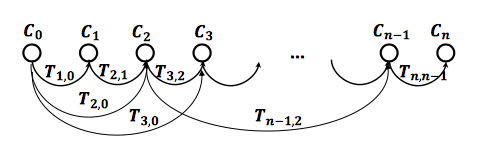
\includegraphics[scale=0.5]{pics/pose}
\caption{Pose graph optimization.}
\end{center}
\end{figure}
\subsubsection*{Bundle Adjustment (BA)}
This incorporates the knowledge of landmarks (3D points).  
\begin{equation}
X^i,C_k=\text{argmin}_{X^i,C_k} \sum_{i} \sum_{k}\rho \left( p_k^i-\pi(X^i,C_k)\right).
\end{equation}
Outliers are a problem, how can we penalize them? In order to penalize wrong matches, we can juse the Huber or Turkey cost.
\begin{equation}
\begin{split}
\text{\textbf{Huber}} \qquad \rho(x)&=\begin{cases}
x^2, &if \ |x|\leq k\\
k\cdot (2|x|-k)& if \ |x| \geq k \text{ linear}
\end{cases}\\
\text{\textbf{Tukey}} \qquad \rho(x)&=\begin{cases}
\alpha^2&if \ |x|\geq \alpha \\
\alpha^2 \cdot \left(1-(1-(\frac{x}{\alpha})^2)^3 \right)&if \ |x|\leq \alpha.
\end{cases}
\end{split}
\end{equation}

\subsubsection*{Bundle Adjustment vs Pose-graph Optimization}
\begin{itemize}
\item BA is more precise than pose-graph optimization because it adds additional constraints (landmark constraints).
\item But \textbf{more costly}: $O((qM+lN)^3)$ with $M$ and $N$ being the number of points and camera poses and $q$ and $l$ the number of parameters for points and camera poses. The Jacobian is cubic in $q$ and $l$. Workarounds are
\begin{itemize}
\item A small window size limits the number of parameters for the optimization and thus makes real-time bundle adjustment possible.
\item It is possible to reduce the computational complexity by just optimizing the camera parameters and keeping the 3D landmarks fixed, e.g. \textbf{freeze the 3D points and adjust the poses}
\end{itemize}
\end{itemize}
\begin{figure}[tbh]
\begin{center}
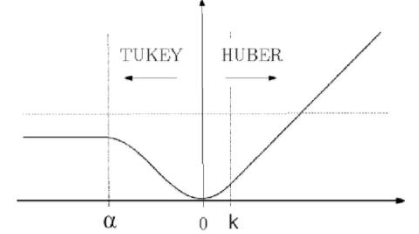
\includegraphics[scale=0.5]{pics/tukey}
\caption{Tukey vs. Huber norm.}
\end{center}
\end{figure}

\begin{figure}[tbh]
\begin{center}
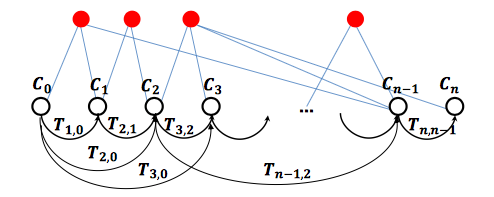
\includegraphics[scale=0.5]{pics/bundle}
\caption{Bundle Adjustment.}
\end{center}
\end{figure}
\end{answer}
\end{enumerate}
\end{enumerate}
\newpage
\section*{Lecture 02/03}
\begin{enumerate}
\item \textit{Blur Circle}
\begin{answer}
In optics, a circle of confusion (or blur circle) is an optical spot caused by a cone of light rays from a lens, not coming to a perfect focus when imaging a point source. 
\begin{itemize}
\item There is a specific distance from the lens at which world points are in focus in the image.
\item Other points project to a \textbf{blur circle} in the image with radius
\begin{equation}
R=\frac{L\delta }{2e}
\end{equation}
$\rightarrow$ a minimal pinhole gives minimal $R$ and\\
$\rightarrow$ $R$ should remain smaller than image resolution.
\end{itemize}
\begin{figure}[h!]
\begin{center}
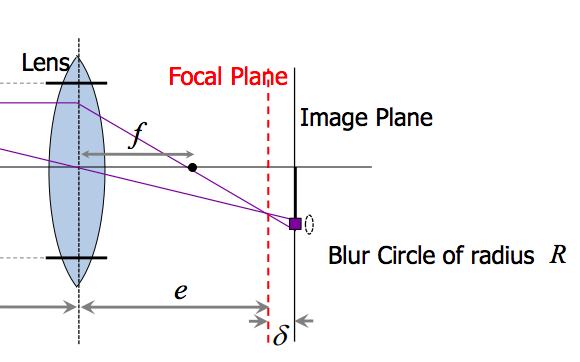
\includegraphics[scale=0.5]{pics/blur_circle}
\caption{Blur Circle  \label{fig:blurcircle}}
\end{center}
\end{figure}
\end{answer}

\item \textit{Thin Lens Equation and Pinhole Approximation}
\begin{answer}
Starting from Figure \ref{fig:focal}, one can use similar triangles and write
\begin{equation}
\begin{split}
\frac{B}{A}&=\frac{e}{z} \text{ and}\\
\frac{B}{A}&=\frac{e-f}{f}=\frac{e}{f}-1.\\
\end{split}
\end{equation}
Toghether, we get the \textbf{thin lens equation}.
\begin{equation}
\frac{e}{f}-1=\frac{e}{z}
\end{equation}
By dividing the thin lens equation by parameter $e$ and considering $z>>f$ we get
\begin{equation}
\begin{split}
\frac{1}{z}&=\frac{1}{f}-\frac{1}{e}\\
0&=\frac{1}{f}-\frac{1}{e}\\
e&\approx f
\end{split}
\end{equation}

\begin{figure}[h!]
\begin{center}
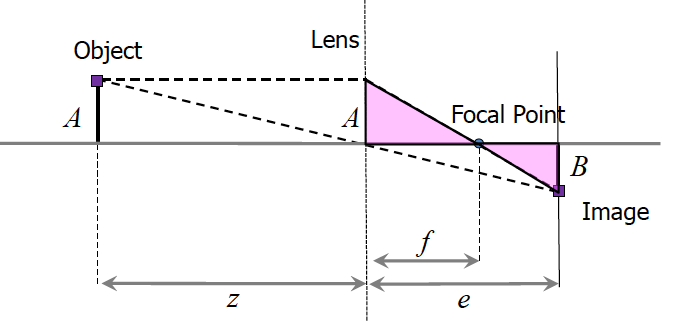
\includegraphics[scale=0.5]{pics/focal}
\caption{Thin lens \label{fig:focal}}
\end{center}
\end{figure}
\end{answer}

\item \begin{enumerate}
\item \textit{Definition of vanishing points and lines}
\begin{answer}
\
\begin{itemize}
\item Straight lines are still straight.
\item Length and angles are lost.
\item Parallel lines in the world intersect in the image as a \textbf{vanishing point}.
\item Parallel planes in the world intersect in the image at a \textbf{vanishing line}. 
\end{itemize}
\end{answer}
\item \textit{Prove that the parallel lines intersect at vanishing points and show how to compute it mathematically.}
\begin{answer}
\begin{claim}
World's parallel lines intersect at a vanishing point in the camera image.
\end{claim}
\begin{proof}
Let's define two parallel 3D lines:
\begin{equation}
\begin{split}
\begin{pmatrix}
X\\
Y\\
Z
\end{pmatrix}&=\begin{pmatrix}
X_1\\
Y_1\\
Z_1
\end{pmatrix}+s\cdot \begin{pmatrix}
l\\
m\\
n
\end{pmatrix},\\
\begin{pmatrix}
X\\
Y\\
Z
\end{pmatrix}&=\begin{pmatrix}
X_2\\
Y_2\\
Z_2
\end{pmatrix}+s\cdot \begin{pmatrix}
l\\
m\\
n
\end{pmatrix}.
\end{split}
\end{equation}
The perspective projection equation in calibrated coordinates are
\begin{equation}
\begin{split}
x&=\frac{X}{Z}\\
y&=\frac{Y}{Z}.
\end{split}
\end{equation}
Plugging the line equations into the perspective projection equation and letting $s\rightarrow \infty$ results in
\begin{equation}
\begin{split}
\lim_{s\rightarrow \infty} \frac{X_i+sl}{Z_i+sn}&=\frac{l}{n}=x_{VP}\\
\lim_{s\rightarrow \infty} \frac{Y_i+sm}{Z_i+sn}&=\frac{m}{n}=y_{VP}.
\end{split}
\end{equation}
This result depends only on the direction vector of the line.
\end{proof}
\end{answer}
\end{enumerate}
In Figure \ref{fig:vanish} another proof is displayed, the lines intersect to a point at infinity and the projection of such point in the image returns the vanishing point \textbf{v}. \textbf{v} is related to \textbf{d} via Eq. 24, where K is the camera matrix. Eq. 25 guarantees that d has unit norm.\\
\begin{figure}[h!]
\begin{center}
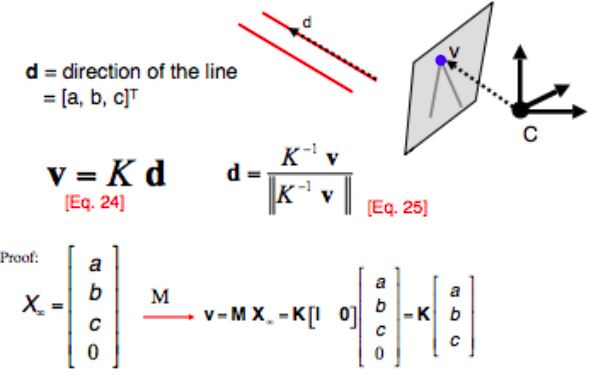
\includegraphics[scale=0.4]{pics/vanish}
\caption{Vanishing point \label{fig:vanish}}
\end{center}
\end{figure}

\item \textit{How do you build an Ames room (the floor and the walls); try to sketch a concept}
\begin{answer}
Have a look at Figure \ref{fig:ames}
\begin{figure}[h!]
\begin{center}
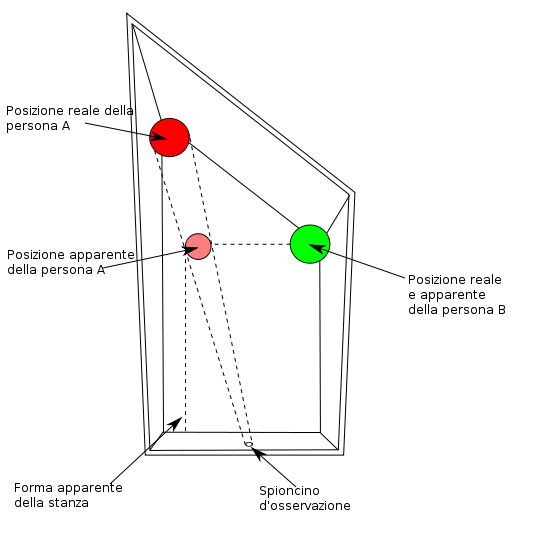
\includegraphics[scale=0.45]{pics/ames}
\caption{Thin lens \label{fig:ames}}
\end{center}
\end{figure}
\end{answer}

\item \textbf{Relation between field of view and focal length.}
\begin{answer}
With Figure \ref{fig:wide}, one can compute the \textbf{field of view}
\begin{figure}[h!]
\begin{center}
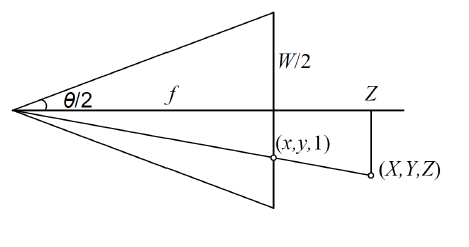
\includegraphics[scale=0.5]{pics/wide}
\caption{Scheme for angles. \label{fig:wide}}
\end{center}
\end{figure}
\begin{equation}
\tan\left( \frac{\theta}{2}\right)=\frac{W}{2f} \Rightarrow f=\frac{W}{2}\left[ \tan \left( \frac{\theta}{2}\right)\right]^{-1}
\end{equation}
$\rightarrow$ smaller FOV = larger focal length.
\end{answer}
\item \begin{enumerate}
\item \textit{Perspective projection equations including lens distortion and world to camera projection (derivation of perspective equations in matrix form using homogeneous coordinates).}
\begin{answer}
The procedure reads
\begin{enumerate}
\item Change of coordinates from 3D world point $P_w$ to 2D camera frame point $P_c$  .
\item Projection from the camera frame to the image plane (x, y).
\item Change in pixel (u, v).
\end{enumerate}
\begin{figure}[h!]
\begin{center}
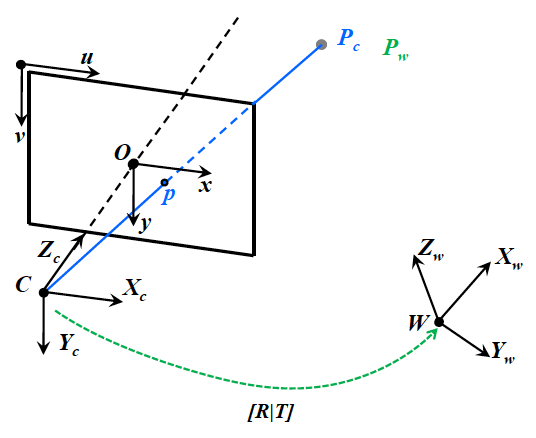
\includegraphics[scale=0.3]{pics/perspective}
\caption{Frames. $Z_c=$ optical axis \label{fig:perspective}}
\end{center}
\end{figure}
\textbf{Perspective Projection }\\
From similar triangles and Figure \ref{fig:proj} one gets from Camera Point $P_c$ to \textbf{image plane} coords
\begin{equation}
\begin{split}
\frac{x}{f}&=\frac{X_c}{Z_c} \Rightarrow x=\frac{fX_c}{Z_c}\\
\frac{y}{f}&=\frac{Y_c}{Z_c} \Rightarrow y=\frac{fY_c}{Z_c}
\end{split}
\end{equation}
\begin{figure}[h!]
\begin{center}
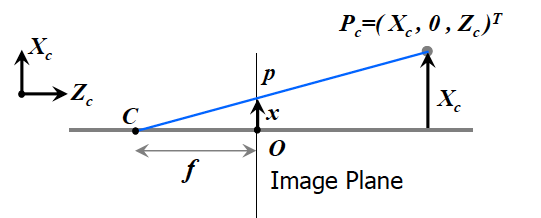
\includegraphics[scale=0.5]{pics/proj}
\caption{Figure for perspective projection. \label{fig:proj}}
\end{center}
\end{figure}
\textbf{Pixel Coordinates}\\
From local \textbf{image plane} coords $(x,y)$ to the \textbf{pixel} coords $(u,v)$ with scale factors $k_u , k_v$ and pixel coords of the camera optical center $O=(u_0,v_0)$:
\begin{equation}\label{img2pix}
\begin{split}
u&=u_0+k_ux \Rightarrow u=u_0+\frac{k_ufX_c}{Z_c}\\
v&=v_0+k_ux \Rightarrow v=v_0+\frac{k_vfX_c}{Z_c}
\end{split}
\end{equation}
\textbf{Homogeneous} coords for linear mapping from 3D $\rightarrow$ 2D by introducing an extra scalar element (the depth of the scene point $\lambda=Z_c$) 
\begin{equation}\label{homog}
p= \underbrace{\begin{pmatrix}
u \\
v
\end{pmatrix}}_{pixel}\rightarrow 
\tilde{p}= 
\underbrace{\begin{bmatrix}
\tilde{u} \\
\tilde{v}\\
\tilde{w}
\end{bmatrix}}_{homog.}=\lambda
\begin{bmatrix}
u \\
v\\
1
\end{bmatrix}
\end{equation}
with \eqref{img2pix} and \eqref{homog} expressed in matrix form reads
\begin{equation}
\begin{pmatrix}
\lambda u\\
\lambda v\\
\lambda 
\end{pmatrix}=\begin{pmatrix}
\alpha _u&0&u_0\\
0&\alpha_v &v_0 \\
0&0&1
\end{pmatrix}\cdot \begin{pmatrix}
X_c\\
Y_c\\
Z_c
\end{pmatrix}=K\begin{pmatrix}
X_c\\
Y_c\\
Z_c
\end{pmatrix},
\end{equation}
with $\alpha _u,\alpha_v$ focal lengths in pixels and $K$ \textbf{calibration matrix}.

 At the end, it holds
\begin{equation}
\lambda \cdot \begin{pmatrix}
u\\
v\\
1
\end{pmatrix}=\underbrace{(K)}_{3\times 3,\ intrinsic}\cdot \underbrace{(\mathbb{I}_{3\times 3}|0)}_{3\times 4}\cdot \underbrace{\begin{pmatrix}
 R&\vec{t} \ \\
 0&1
\end{pmatrix}}_{4\times 4, \ extrinsic}\cdot \begin{pmatrix}
X_w\\
Y_w\\
Z_w\\
1
\end{pmatrix}.
\end{equation}
We use the notation from homogeneous to euclidean:
\begin{equation}
\underbrace{\begin{pmatrix}
u \\
v\\
w
\end{pmatrix}}_{Homog.}\rightarrow 
\underbrace{\begin{pmatrix}
u/w \\
v/w\\
1
\end{pmatrix}}_{Eucl.}
\end{equation}
\textbf{Radial Distortion}
This is a transformation from ideal to distorted coordinates. For most lenses, one writes
\begin{equation}
\begin{pmatrix}
u_d\\
v_d
\end{pmatrix}=\underbrace{(1+k_1r^2)}_{\text{\parbox{10em}{higher order dep on amount of distortion $r^4$ etc.}}}\cdot \begin{pmatrix}
 u-u_0\\
 v-v_0
 \end{pmatrix}+\begin{pmatrix}
u_0\\
v_0
\end{pmatrix},
\end{equation}
with
\begin{equation}
r^2=(u-u_0)^2+(v-v_0)^2.
\end{equation}
Based on the Brown-Conrady model. \textbf{Barrel} distortion has distortion coef $k_1<0$. 
\textbf{Ask someone:} what is the relation between order of the term to the amount of distortion????
\end{answer}
\item \textit{Normalized image coordinates and geometric explanation.}
\end{enumerate}
\item \begin{enumerate}
\item \textit{Definition of general PnP problem (what’s the minimum number of points and what are the degenerate configurations).}
\begin{answer}
Given the realitve spatial locations of $n$ control points and given the angle to every pair of control points from an additional point called the Center of Perspective $C_P$, find the lengths of the line segments joining $C_P$ to each of the control points.\\
We assume we know the camera intrinsic parameters. Given known 3D landmarks in the world and their image correspondence in the camera frame, determine the 6DOF pose of the camera in the world frame. \textbf{Where is the camera?}
\begin{itemize}
\item Given 1 point: $\infty$ solutions.
\item Given 2 points: $\infty$ \textit{bounded} solutions.
\item Given 3 \textbf{non collinear} points: Finitely many (up to 4) solutions.
\item Given 4 points: unique solution.
\end{itemize}
With 3 points one can use the fact that the angles inscribed in the triangle are the same: the Carnot's theorem reads
\begin{equation}
s_{1,2,3}^2=L_{B,A,A}^2+L_{C,C,B}^2-2L_{B,A,A}L_{C,C,B}\cos(\theta_{BC,AC,AB})
\end{equation}
In general, $n$ independent polynomials with $n$ unknowns, can have no more solution than the \textbf{product} of their degrees: here 8. \\
$\rightarrow$ fourth point to \textbf{disambiguate} the solutions! By defining $x=\frac{L_B}{L_A}$ we can reduce the system to a $4^{th}$ order equation
\begin{equation}
G_0+G_1x+G_2x^2+G_3x^3+G_4x^4=0.
\end{equation}
This applies to camera pose estimation from known $3D-2D$ correspondences (e.g. hololens).
\begin{itemize}
\item L: distance from Camera frame origin C to World point A,B,C
\item $\theta$: inscribed angles between e.g.  $L_A$ and $L_B$
\item s: distance between World points e.g. A and B
\end{itemize}
\end{answer}

\item \textit{Working principle of P3P algorithm (non-linear algorithm for calibrated cameras: what are the algebraic trigonometric equations that it attempts to solve?).}
\item \textit{How do we solve PnP using a linear algorithm (derive DLT equations for 3D object or planar grids) and what is the minimum number of point correspondences it requires, why?}
\begin{answer}
\subsubsection*{Direct Linear Transform}
\begin{equation}
\begin{split}
\text{image point}=\tilde{p}&=\begin{pmatrix}
\tilde{u}\\
\tilde{v}\\
\tilde{w}
\end{pmatrix} = \lambda \begin{pmatrix}
 u\\
 v\\
 1
 \end{pmatrix}=K[R|T]\cdot \begin{pmatrix}
 X_w\\
 Y_w\\
 Z_w\\
 1
 \end{pmatrix}\\
 &=\begin{pmatrix}
\alpha_u &0&u_0\\
0&\alpha_v &v_0\\
0&0&1
\end{pmatrix}\cdot \begin{pmatrix}
 r_{11}&r_{12}&r_{13}&t_1\\
 r_{21}&r_{22}&r_{23}&t_2\\
 r_{31}&r_{32}&r_{33}&t_3
 \end{pmatrix}\cdot \begin{pmatrix}
 X_w\\
 Y_w\\
 Z_w\\
 1
 \end{pmatrix}\\
\textit{assuming indep. elements} \qquad &=\underbrace{\begin{pmatrix}
 m_{11}&m_{12}&m_{13}&m_{14}\\
 m_{21}&m_{22}&m_{23}&m_{24}\\
 m_{31}&m_{32}&m_{33}&m_{34}
 \end{pmatrix}}_{M}\cdot \begin{pmatrix}
 X_w\\
 Y_w\\
 Z_w\\
 1
 \end{pmatrix}\\
 &=\begin{pmatrix}
m_1^T\\
m_2^T\\
m_3^T
\end{pmatrix}\cdot \underbrace{\begin{pmatrix}
 X_w\\
 Y_w\\
 Z_w\\
 1
 \end{pmatrix}}_{P}.
 \end{split}
\end{equation}
It follows
\begin{equation}
\begin{split}
u&=\frac{\tilde{u}}{\tilde{w}}=\frac{m_1^T\cdot P}{m_3^T\cdot P}\\
v&=\frac{\tilde{v}}{\tilde{w}}=\frac{m_2^T\cdot P}{m_3^T\cdot P}
\end{split}
\end{equation}
and hence
\begin{equation}
\begin{split}
(m_1^T-u_im_3^T)\cdot P_i&=0\\
(m_2^T-v_im_3^T)\cdot P_i&=0.
\end{split}
\end{equation}
Rearranging the terms you have
\begin{equation}
\begin{pmatrix}
P_1^T &0^T&-u_1P_1^T\\
0^T&P_1^T&-v_1P_1^T\\
\end{pmatrix}\cdot \begin{pmatrix}
 m_1\\
 m_2\\
 m_3
 \end{pmatrix}=\begin{pmatrix}
0\\
0
\end{pmatrix}.
\end{equation}
For $n$ points we have a big $2n \times 12$ matrix $Q$.\\ The problem hence reads
\begin{equation}
Q\cdot M=0,
\end{equation}
where $Q$ is known and $M$ is unknown. \\ \\
\textbf{Minimal Solution:}
\begin{itemize}
\item Rank 11 to have unique non-trivial (up to scale)  solution $M$ ($Q$ known!).
\item Each 3D/2D correspondence provides 2 independent equations.
\item $5+\frac{1}{2}$ correspondences are needed (in fact 6).
\end{itemize}
\textbf{Overdetermined Solution:}
\begin{itemize}
\item More than 6 points.
\item Minimize $||QM||^2$ with the constraint $||M||=1$ $\rightarrow$ SVD. The solution is the eigenvector corresponding to the smallest eigenvalue of $Q^TQ$. That's because this is the unit vector $x$ that minimizes $||Qx||^2=x^TQ^TQx$. This can be done in matlab with
\begin{verbatim}
[U,S,V] = svd(Q);
 M = V(:,12);
\end{verbatim}

\end{itemize}
\textbf{Degenerated Configurations:}
\begin{itemize}
\item Points lying on a plane and or along a line passing through the projection center.
\item Camera and points on a twisted cubic (degree 3).
\end{itemize}
Once we have $M$, we know from its definition
\begin{equation}
M=K(R|T).
\end{equation}
\begin{bmk}
\
\begin{itemize}
\item We are not enforcing orthogonality of $R$.
\item QR factorization of $M$, whith $R$ (orth.) and $T$ (upper triangular matrix). 
\item Or: Using SVD and enforcing that every eigenvalue is 1.
\item We can estimate the scale factor (M comes with a scale factor) by dividing the Frobenius norm of the computed matrix $\tilde{R}$ with the one of the current estimate.
\end{itemize}
\end{bmk}
\end{answer}
\subsubsection*{DLT vs. PnP}
\begin{itemize}
\item If the camera is calibrated, only $R$ and $T$ need to be determined. PnP leads to smaller error regarding calibration using same number of points to estimate pose.
\item PnP's computation time is quite constant with increasing number of points, while DLT's computation time increases with the increasing number of points.
\end{itemize}
\end{enumerate}
\item \begin{enumerate}
\item \textit{Omnidirectional cameras (only definition of central and non central cameras):}
\begin{answer}
A vision system is said to be central when the optical rays of the viewed objects intersect in a single point in 3D called projection center or \textbf{single effective viewpoint}. For hyperbolic and elliptical mirrors, the single viewpoint property is achieved by ensuring that the camera center coincides with one of the foci of the hyperbola (ellipse), as reported in Figure \ref{fig:fuochi}.
 The camera is \textbf{non-central}, if the rays intersect in various points. 
 \begin{figure}[tbh]
\begin{center}
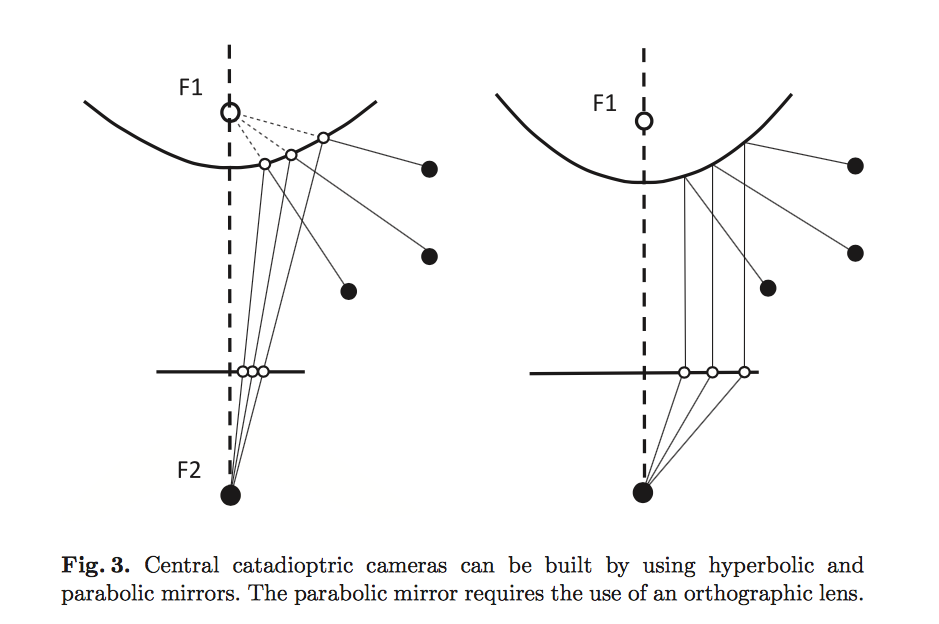
\includegraphics[scale=0.35]{pics/fuochi}
\caption{Central Catadioptric cameras\label{fig:fuochi}}
\end{center}
\end{figure}
\end{answer}
\item \textit{What type of mirror ensure central projection?}
\begin{answer}
Class of rotated (swept) conic shapes: hyperbolical, parabolical, elliptical mirrors ensure central projection.
\end{answer}
\item \textit{Spherical model: illustrate equivalence between perspective and omnidirectional model.}
\begin{answer}
With their landmark paper from 2000, Geyer and Daniilidis showed that every catadioptric (parabolic, hyperbolic, elliptical) and standard perspective projection is equivalent to a projective mapping from a sphere, centered in the single viewpoint, to a plane with the projection center on the perpendicular to the plane and distant $\varepsilon$ from the center of the sphere, as you can see in Figure \ref{fig:sphere}. Let $P=(x,y,z)$ be a scene point in the mirror reference frame centered in $C$. We assume that the axis of symmetry of the mirror is perfectly aligned with the optical axis of the camera. We also assume that the $x$ and $y$ axes of the camera and mirror are aligned. Therefore, the camera and mirror frames differ only by a translation along $z$.
 \begin{figure}[tbh]
\begin{center}
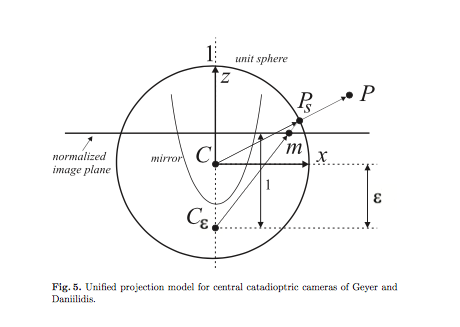
\includegraphics[scale=0.6]{pics/sphere}
\caption{Spherical Model\label{fig:sphere}}
\end{center}
\end{figure}
\begin{enumerate}
\item Projecting the image point $P=(x,y,z)$ from the \textbf{ mirror reference frame} to the \textbf{unit sphere}
\begin{equation}\label{nomalize P to unit sphere}
P_s=\frac{P}{\Vert P \Vert}=(x_s,y_s,z_s)
\end{equation}
\item The point coordinatess are converted to the coordinates of the \textbf{new} reference frame centered in $C_\varepsilon = (0,0,-\varepsilon) : P_\varepsilon =(x_s,y_s,z_s+\varepsilon)$. We can observe that $\varepsilon$ ranges between 0 (\textit{planar} mirror ) and 1 (\textit{parabolic mirror}). Its exact value can be obtained by knowing the distance $d$ between the foci and the latus rectum $l$.
\item Project the point $P_\varepsilon$ onto the \textbf{ normalized image plane} distant 1 from $C_\varepsilon$ 
\begin{equation}\label{projection to norm image plane}
\tilde{m}=(x_m,y_m,1)=\left(\frac{x_s}{z_s+\varepsilon}, \frac{y_s}{z_s+\varepsilon},1\right)= g^{-1} (P_s)
\end{equation}
\item Point $\tilde{m}$ is mapped to the \textbf{camera} image point $\tilde{p}=(u,v,1)$ through K $\rightarrow \tilde{p}= K\cdot \tilde{m}$, where K is given by 
\begin{equation}
K=\begin{pmatrix}
\alpha_u &\alpha_u \cot(\theta)&u_0\\
0&\alpha_v &v_0\\
0&0&1
\end{pmatrix}.
\end{equation}
By inverting $g$ given by Eq. \ref{projection to norm image plane}, we can project points from the normalized image plane back to the  \textbf{unit sphere}
\begin{equation}\label{inverse g}
P_s= g(m) \sim \begin{bmatrix}
x_m\\
y_m\\
1-\varepsilon\frac{x_m^2+y_m^2+1}{\varepsilon+\sqrt{1+(1-\varepsilon^2)(x_m^2+y_m^2)}}
\end{bmatrix}
\end{equation} 
Note that the last row of $P_s$ is obtained by imposing that $P_s$ lies on the sphere, i.e. $x_s+y_s+z_s=1$
\end{enumerate}
Eq.  \ref{inverse g} is the core of the projection model of \textbf{central catadioptric} camera. In case of a planar mirror, $\varepsilon$ center of a sphere = 0, Eq. \ref{inverse g} is the same projection equation of a \textbf{perspective} camera $P_s\sim (x_m,y_m,1)$.
\end{answer}
\item \textit{What do we mean by normalized image coordinates on the unit sphere?}
\begin{answer}
Projecting the image point $P=(x,y,z)$ from the \textbf{ mirror reference frame} to the  \textbf{unit sphere} using Eq.  \ref{nomalize P to unit sphere}.
\end{answer}
\end{enumerate}
\item \textit{Given an image and the associated camera pose, how would you superimpose a virtual object on the image (for example, a virtual cube). Describe the steps involved.}
\begin{answer}
For undistorted images:
\begin{enumerate}
\item Convert the image to grayscale
\item Create a matrix containing all the 3D positions of the checkerboard corners (meshgrid).
\item Write a function to project the corners on the image plane (maps points from the world to the camera frame).
\begin{itemize}
\item From matrix $K$ one can recover the rotation matrix $R$ with the Rodriguez formula
\begin{equation}
R=\mathbb{I}+\sin(\theta) [k]_{\times}+(1-\cos(\theta))[k]_\times ^2.
\end{equation}
\item The camera poses are the vector $t$.
\item Find the normalized coordinates (divide by third component of the vector).
\item Convert to pixel coordinates applying $K$, i.e. $K\cdot x_{\text{dist}}$.
\end{itemize}
\item Undistort images with bilinear transformation.
:
\begin{itemize}
\item Artifacts due to the facts that some coordinates are non-integer. This is usually solved by backward warping: warping pixel locations from destination image (undistorted) to source image (distorted: 
\begin{equation}
I_u(u,v)=I_d(\Gamma(u,v)).
\end{equation}
To deal with non-integers, we use nearest neighbor interpolation (closest integer). Short explanation: \\
\textit{When an image needs to be scaled up, each pixel of the original image needs to be moved in a certain direction based on the scale constant. However, when scaling up an image by a non-integral scale factor, there are pixels (i.e., holes) that are not assigned appropriate pixel values. In this case, those holes should be assigned appropriate RGB or grayscale values so that the output image does not have non-valued pixels.
Bilinear interpolation can be used where perfect image transformation with pixel matching is impossible, so that one can calculate and assign appropriate intensity values to pixels. Unlike other interpolation techniques such as nearest-neighbor interpolation and bicubic interpolation, bilinear interpolation uses values of only the 4 nearest pixels, located in diagonal directions from a given pixel, in order to find the appropriate color intensity values of that pixel.
Bilinear interpolation considers the closest 2 $\times 2$ neighborhood of known pixel values surrounding the unknown pixel's computed location. It then takes a weighted average of these 4 pixels to arrive at its final, interpolated value}
\end{itemize}
\item Define the world points of the cube vertex and then project them using the same transform as before.
\end{enumerate}
\end{answer}

\end{enumerate}



\newpage
\section*{Lecture 04 }
\subsection*{Filtering}
\begin{enumerate}
\item \textit{Convolution vs correlation}
\begin{answer}
Correlation is a metric for similarity between two different signals. Convolutions applies one signal to the other. \\
\textbf{Convolution}:One of the sequences is flipped before sliding over the other. The resulting sequence expresses the amount of overlap of one sequence when it is shifted over another sequence. Linearity, associativity, commutativity. Notation $f*g$. In 1D:
\begin{equation}
f*g=\int_{-\infty}^{\infty}f(\tau)g(t-\tau)\text{d}\tau.
\end{equation}
Here g is reversed and shifted over f.\\
In 2D:
\begin{equation}
\begin{split}
G[i,j]&=H*F\\
&=\sum_{u=-k}^k\sum_{v=-k}^{k} H[u,v]F[i-u,j-v].
\end{split}
\end{equation}
Flip the filter in both dimensions, then slide the filter over the image. In other words: replacing each pixel with a linear combination of its neighbors. The filter $H$ is also called kernel or mask. One can change the weights.\\
\textbf{Correlation}: no flipping before shifting and displays the measure of similarity between the two sequence, sliding dot product, used in pattern recognition
\begin{figure}[h!]
\begin{center}
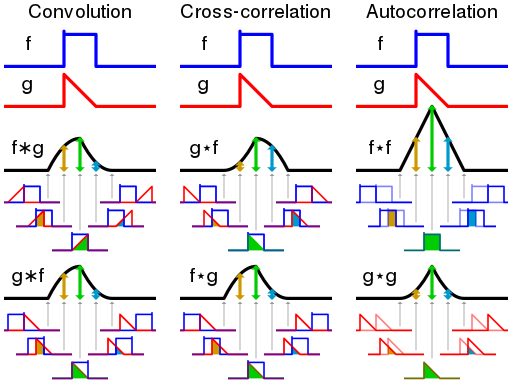
\includegraphics[scale=0.4]{pics/convolution}
\caption{Convolution. Cross-correlation. Autocorrelation \label{convolution}}
\end{center}
\end{figure}
\end{answer}
\item \textit{Box filter vs Gaussian filter (what are the pros and cons of either one?)}
\begin{answer}
\
\textbf{Box Filter}: spatial domain linear filter in which each pixel in the resulting image has a value equal to the average value of its neighboring pixels in the input image.
\begin{enumerate}
\item low pass filter (blur)
\item mask with positive entries that sum to 1 
\item all weights are equal
\item size : $m\times m$
\item $+$: faster than sliding window algorithm
\item $-$: aliasing, blurs out details stronger than Gaussian Filter
\end{enumerate}
\textbf{Gaussian Filter}: 
What if we want the \textbf{closest} pixels to have a higher influence on the output? More weight on the central pixels, less to the neighbors. (non-uniform low pass filter)
\begin{equation}
h(u,v)=\frac{1}{2\pi \sigma^2}e^{-\frac{u^2+v^2}{2\sigma^2}}.
\end{equation}
\begin{itemize}
\item $+$: fastest filter from the 3
\item $-$: blurs edges and reduces contrast
\end{itemize}
What parameter matter? 
\begin{itemize}
\item Size of the kernel. The Gaussian has generally infinite support but discrete filters use finite kernels. 
\item The \textbf{variance} $\sigma^2$ of Gaussian: determines extent of smoothing (larger variance, larger smoothing).
\end{itemize}
\end{answer}
\item \textit{Gaussian filters: why should we increase the size of the kernel if sigma is large (i.e. sigma close to the size of the filter kernel?)}
\begin{answer}
Maintain the Gaussian nature of the filter. If $\sigma$ too close to size of the kernel, the coefficient at the edge of the mask is not close to 0. $\rightarrow$ abrupt change, not rotational symmetric .
\end{answer}
\item \textit{Median filter (when do we need a median filter?)}
\begin{answer}
Removes spikes: good for impulse and salt and pepper noise (linear smoothing filters do not alleviate that, random high values create high value patches). \\
Nonlinear filter, which computes the median value and replaces the high value with that. 
\begin{itemize}
\item $+$: Preserves sharp transitions/ edges.
\item $-$: Removes small brightness variations.
\end{itemize}
\end{answer}
\item \textit{Boundary issues}
\begin{answer}
The filter window falls off the edge of the image. We need to pad the image borders with
\begin{itemize}
\item Zero padding (black)
\item Wrap around
\item Copy edge
\item Reflect across edge
\end{itemize}
\end{answer}
\end{enumerate}

\subsection*{Edge Detection}
\begin{enumerate}
\item \textit{Working principle with 1D signal}
\begin{answer}
Edges are nothing else than sharp intensity changes. The intensity function along a horizontal scan line $f(x)$ has low values for dark parts. Taking the first derivative of the intensity function, edges correspond to \textbf{extrema of derivative}.
\end{answer}
\item \textit{Noise effects}
\begin{answer}
Considering only a single row or column of the image, if the image has a lot of noise, the first derivative is even noisier. Hence, we cannot see the edge in the change of intensity. In practice, differenciating a noisy signal leads to too many peaks. Solution: first smooth the image (convolution with $h$), then differentiate.
\end{answer}
\item \textit{Differential property of convolution}
\begin{answer}
\begin{equation}
\frac{\partial}{\partial x}(h\star f) = (\frac{\partial}{\partial x}h) \star f
\end{equation}
First derive the filter $h(x)$, then convolution. Smoothed and derived to detect the noisy intensity function $f$.
\end{answer}
\item \textit{How do we compute the first derivative along x and y?}
\begin{answer}
For discrete data, it holds
\begin{equation}
\frac{\text{d}f(x,y)}{\text{d}x}\approx \frac{f(x+1,y)-f(x,y)}{1}.
\end{equation}
Partial derivatives of an image are in $x$ (-1,1), in $y$ $\begin{pmatrix} -1\\1 \end{pmatrix}$. 
The \textbf{Gradient} of an image if given by 
\begin{equation}
\nabla f=\begin{pmatrix} 
\frac{\partial f}{\partial x}&\frac{\partial f}{\partial y}
\end{pmatrix}
\end{equation}
The \textbf{gradient direction} is given as
\begin{equation}
\Theta = \tan^{-1}\left( \frac{\frac{\partial f}{\partial y}}{\frac{\partial f}{\partial x}}\right).
\end{equation}
The \textbf{edge strength} is given by
\begin{equation}
||\nabla f||=\sqrt{(\frac{\partial f}{\partial y})^2+(\frac{\partial f}{\partial y})^2}.
\end{equation}
First smoothing with a Gaussian (or other filter), then taking directional derivative \textbf{equals} convolving image with a Sobel filter = \textit{directional/ oriented} filter or first take directional derivative of the Gaussian filter,the convolve the image with the derivative.
\end{answer}
\item \textit{Laplacian of Gaussian operator: why should we use it and what effect does it have on the image?}
\begin{answer}
This operator is separable. It can be split into directions. Consider
\begin{equation}
\frac{\partial ^2}{\partial x^2}(h \star f)
\end{equation}
From above we know the Gaussian filter smooths the image and then taking the derivatives \textbf{equals} convolving the image directly with the \textit{Laplacian of Gaussian} (LoG) filter. Taking the second derivative of the filter, it acts as a \textit{band-pass filter} which filters out both low and high frequencies.
\end{answer}
\item \textit{Properties of smoothing and derivative filters (what is the sum of the coefficients of a smoothing filter, and of a derivative filter?)}
\begin{answer}
\
\textbf{Smoothing Filter}
\begin{itemize}
\item Has positive values
\item Sums to 1$\rightarrow$ preserves brightness of constant regions
\item Removes high frequency components.
\end{itemize}
\textbf{Derivative Filter}
\begin{itemize}
\item Has opposite signs, used to get high response in regions of high constrast.
\item Sums to 0 $\rightarrow$ no response in constant regions. If not, uniform zones would have a gradient in spatial domain, which is not what we want.
\item Highlights high frequency components.
\end{itemize}
\end{answer}
\item \textit{Illustrate Canny edge detection.}
\begin{answer}
The process of Canny edge detection algorithm
\begin{enumerate}
\item Convert colour image to grayscale by replacing each pixel by the mean value of its RGB components
\item Apply Gaussian filter to smooth the image in order to remove the noise
\item Compute the gradient of the smoothed image in both directions.  
(or replace step 2. and 3. by convolving the image with $x$ and $y$ derivatives of Gaussian filters)
\item Discard pixels whose gradient magnitude is below a certain threshold.
\item Apply non-maximal suppression to get rid of spurious response to edge detection
\end{enumerate}
The \textit{scale parameter} $\sigma$ is selected based on
\begin{itemize}
\item the desired level of detail: fine edges vs global edges;
\item the noise level;
\item the localisation-detection trade off: see template matching.
 \end{itemize}
\end{answer}
\item \textit{What is non-maxima suppression and how is it implemented?}
\begin{answer}
The local maxima is tracked along gradient direction. High intensity means high probability of the presence of an edge: this is not enough. Only local maxima can be considered as part of an edge. A local maxima can be found where the gradient derivative is 0. Due to noise and the multiple response, the filtered image may contain wide ridges around the local maxima. 
\begin{enumerate}
\item From each position (x, y), step in the two directions perpendicular to edge orientation $\theta$(x, y).
\item Denote the initial pixel (x, y) by C, the two neighboring pixels in the
perpendicular directions by A and B.
\item  If the M(A) $>$ M(C) or M(B) $>$ M(C), discard the pixel (x, y) by setting M(x, y) = 0.
\end{enumerate}
The non-maxima suppression sets all pixels to zero that are not actually local maxima $\rightarrow$  a \textbf{thin line} in the output. 
\end{answer}
\end{enumerate}
\newpage
\section*{Lecture 05/06}
\subsection*{Point feature detection}
\begin{enumerate}
\item \textit{What is template matching and how is it implemented? (Mathematical expression)}
\begin{answer}
Find location in an image that are similar to a \textbf{template}. If we look at filters as templates, we can use \textbf{correlation} to detect these locations. In the resulting correlation map, the brighter the spots the more the template correlates to something on the image.\\
We consider images $H$ and $F$ as vectors and express the correlation between them as
\begin{equation}
\langle H,F\rangle=||H|| \cdot ||F|| \cdot \cos(\theta).
\end{equation}
If we use \textbf{Normalized Cross Correlation} (NCC) (highest complexity), we consider the unit vectors of $H$ and $F$, hence we measure their similarity based on the angle $\theta$. For identical vectors one gets $NCC=1$. 
\begin{equation}
\begin{split}
\cos(\theta)&=\frac{\langle H,F \rangle}{||H||\cdot ||F||}\\
&=\frac{\sum_{u=-k}^{k}\sum_{v=-k}^{k}H(u,v)F(u,v)}{\sqrt{\sum_{u=-k}^{k}\sum_{v=-k}^{k}H(u,v)^2}+\sqrt{\sum_{u=-k}^{k}\sum_{v=-k}^{k}F(u,v)^2}}>0.8.
\end{split}
\end{equation}
\end{answer}
\item \textit{What are the limitations of template matching? Can I use it to recognize any car?}
\begin{answer}
Template Matching will only work if \textbf{scale, orientation, illumination} and in general the appearance of the template and the object to detect are very similar. Hence, this process can only detect cars very similar to the template car, but not generally cars. $\rightarrow$ \textbf{can't use to recognize any car}.
\end{answer}
\item \textit{Similarity metrics: SSD, SAD, NCC, Census transform. What is the intuitive explanation behind SSD and NCC (hint: represent images as vectors)?}
\begin{answer}

\begin{itemize}
\
\item The \textbf{normalized cross correlation (NCC)} takes values between -1 and 1, 1 equals identical. NCC is invariant to linear intensity changes! It holds
\begin{equation}
\begin{split}
NCC&=\frac{\langle H,F \rangle}{||H||\cdot ||F||}\\
&=\frac{\sum_{u=-k}^{k}\sum_{v=-k}^{k}H(u,v)F(u,v)}{\sqrt{\sum_{u=-k}^{k}\sum_{v=-k}^{k}H(u,v)^2}+\sqrt{\sum_{u=-k}^{k}\sum_{v=-k}^{k}F(u,v)^2}}.
\end{split}
\end{equation}
\item Other methods are the \textbf{Sum of Absolute Differences (SAD) (simplest)}
\begin{equation}
SAD=\sum_{u=-k}^{k}\sum_{v=-k}^{k}|H(u,v)-F(u,v)|,
\end{equation}
\item the \textbf{Sum of Squared Differences (SSD) (high computational complexity)}
\begin{equation}
SSD=\sum_{u=-k}^{k}\sum_{v=-k}^{k}(H(u,v)-F(u,v))^2.
\end{equation}
\item \textbf{Census Transfrom}: It maps an image patch to a bit string. The general rule is that \textbf{if a pixel is greater than the center pixel} its corresping bit is set to 1, else to 0. For a $n\times n$ window the string will be $n^2-1$ bits long. The 2 bit strings are compared using the \textbf{Hamming distance} (if bigger than previous 1, else 0, starting from right). The \textbf{Advantages} are
\begin{itemize}
\item More \textbf{robust to object background} problem
\item No square roots or divisions are required. Efficient!
\item Intensities are considered relative to the center pixel of the patch making it \textbf{invariant to monotonic intensity} changes.
\end{itemize}
\end{itemize}
SAD and SSD are \textbf{not} invariant to linear illumination changes. To cope with the difference, the mean value of each image can be subtracted: Zero-mean Normalized Cross Correlation is invariant to linear illumination change intensity. \\
The similarity is computed between the gray intensity levels of the two vectors. If $I_1$ and $I_2$ are perfect matches, the resultant SAD and SDD will be 0. \textcolor{red}{Intuition is missing!}

\end{answer}
\item \textit{Feature extraction: what are good feature to track: definition of corners and blobs and their pros and cons.}
\begin{answer}
Good features are always \textbf{perceivable} and easily detectable from the environment. \textbf{Corners, blobs}, lines and points are \textit{low-level features (geometric primitives)}. Better for detection because they 
\begin{itemize}
\item can be abstracted from raw date $\rightarrow$ high conservation of information
\item provide lower volume of data while increasing the distinctiveness of each feature
\end{itemize}

\textbf{Corners}
\begin{itemize}
\item Intersection of one or more edges, image gradient has \textbf{two or more} dominant directions
\item Repeatable and distinctive
\item Examples of corner detectors are Harris, Shi-Tomasi, SUSAN, FAST.
\item $+$: high localization accuracy $\rightarrow$ good for VO
\item $-$: less distinctive than a blob
\item Change of angle between images should be little
\end{itemize}
\textbf{Blob:} 
\begin{itemize}
\item Any other image pattern which is not a corner, that differs significantly from its neighbors in intensity and texture.
\item Examples of blob detectors are MSER, LOG, DOG, SIFT, SURF, CenSurE.
\item $+$: for place recognition because more distinctive than a corner
\item $-$: Localization accuracy
\item Center might shift due to shear
\end{itemize}

\end{answer}
\item \textit{Harris corner detector}: 
\begin{enumerate}
\item \textit{Intuitive illustration using Moravec definition of corner, flat region, and edge}
\begin{answer}
Shifting a window in \textbf{any direction} should give a \textbf{large change} in intensity (e.g. in SDD) in a least 2 directions
\begin{itemize}
\item \textbf{Flat} region: no intensity change! (SSD$\approx$ 0 in all directions).
\item \textbf{Edge}: no change along the edge direction (SSD $\approx$0 along adge but $>>0$ in other directions).
\item \textbf{Corner:} significant change in at least two directions (SSD $>>0$ in at least 2 directions).
\end{itemize}
\end{answer}
\item \textit{Show how to get to the second moment matrix from the definition of SSD and first order approximation (show that this is a quadratic expression) and what is the intuitive interpretation of the second moment matrix using ellipse (what does the ellipse represent?). }
\begin{answer}
Let $I$ be a gray scale image. We consider the reference patch centered at $(x,y)$ and the shifted window centered at $(x+\Delta x,y+\Delta y)$. The patch has size $P$. We compute
\begin{equation}
SSD(\Delta x, \Delta y)=\sum_{x,y \in P}\left( I(x,y)-I(x+\Delta x,y+\Delta y)\right)^2.
\end{equation}
We define
\begin{equation}
I_x=\frac{\partial I(x,y)}{\partial x}, \quad I_y=\frac{\partial I(x,y)}{\partial y},
\end{equation}
and approximate with first order Taylor expansion:
\begin{equation}
\begin{split}
I(x+\Delta x,y+\Delta y) &\approx I(x,y)+I_x(x,y)\Delta x + I_y(x,y)\Delta y\\
&\Rightarrow SSD(\Delta x, \Delta y)\approx \sum_{x,y\in P}\left( I_x(x,y)\Delta x+I_y(x,y)\Delta y\right)^2
\end{split}
\end{equation}
\textbf{Simple quadratic function in the deltas!} We can write this in matrix form:
\begin{equation}
SSD(\Delta x, \Delta y)\approx \begin{pmatrix}
 \Delta x & \Delta y 
 \end{pmatrix}\cdot \underbrace{\sum_{x,y\in P} \begin{pmatrix}
I_x^2&I_xI_y \\ I_xI_y&I_y^2
\end{pmatrix}}_{M}\cdot \begin{pmatrix}
 \Delta x\\
 \Delta y
 \end{pmatrix},
 \end{equation}
 where $M$ is the second moment matrix. The elements from the matrix are \textbf{pixel-wise products}!

\end{answer}
\item \textit{What is the M matrix for an edge, for a flat region, for an axis-aligned 90-degree corner, and for a non-axis- aligned 90-degree corner? }
\begin{answer}
\
\begin{itemize}
\item Edge along $x$: $M=\begin{pmatrix} 0&0\\ 0&\lambda_2
\end{pmatrix}$.
\item Flat region: $M=\begin{pmatrix} 0&0\\ 0&0 \end{pmatrix}$
\item Aligned corner: $M=\begin{pmatrix} \cos(45)&-\sin(45)\\ \sin(45) & \cos(45) \end{pmatrix}\cdot \begin{pmatrix} \lambda_1 &0 \\
0& \lambda_2 \end{pmatrix}\cdot \begin{pmatrix} \cos(45)&\sin(45)\\ -\sin(45) & \cos(45) \end{pmatrix}$
\item Non-axis aligned corner: M is symmetric, decompose it to $M=R^{-1}\begin{pmatrix}
\lambda_1 &0 \\
0  &\lambda_2
\end{pmatrix} R$ where the angle $\neq \pi /4$ in the rotation matrix R
\end{itemize}
\end{answer}
\item \textit{What do the eigenvalues of M reveal? }
\begin{answer}
The Eigenvaluess give information about, if the image patch is an edge or not. The two Eigenvectors identify the directions of largest and smallest changes of SSD. \\
\begin{claim}
One can visualize this as an ellipse with axis lengths determined by eigenvalues ($1/\sqrt{\lambda_\mathrm{max,min}}$) and two axes determined by the eigenvectors of $M$ (columns of $R$). 
\end{claim}
\begin{proof} Since $M$ is symmetric, we can always come to its eigenvalue decomposition. Let's consider \begin{equation}
M=\begin{pmatrix} v_1 &v_2 \end{pmatrix}\cdot \begin{pmatrix}
\lambda_1 &0\\
0&\lambda_2
\end{pmatrix}\cdot \begin{pmatrix}
 v_1^T\\
 v_2^T
 \end{pmatrix}=1
\end{equation}
Then, using the quadratic form one gets 
\begin{equation}
\begin{split}x^T\cdot \begin{pmatrix} v_1 &v_2 \end{pmatrix}\cdot \begin{pmatrix}
\lambda_1 &0\\
0&\lambda_2
\end{pmatrix}\cdot \begin{pmatrix}
 v_1^T\\
 v_2^T
 \end{pmatrix}\cdot x&=1\\
 \lambda_1 x^T v_1  v_1^T  x + \lambda_2 x^T v_2  v_2^Tx&=1\\
 \lambda_1  (v_1^Tx)^T (v_1^Tx)+ \lambda_2 (v_2^Tx)^T (v_2^Tx)&=1\\
 \frac{(v_1^Tx)^2}{\left( \frac{1}{\sqrt{\lambda_1}}\right)^2}+ \frac{(v_2^Tx)^2}{\left (\frac{1}{\sqrt{\lambda_2}}\right)^2}&=1,
\end{split}
\end{equation}
from which is clear that the eigenvectors $v_1,v_2$ represent the axis directions of the ellipse and $\frac{1}{\sqrt{\lambda_1}},\frac{1}{\sqrt{\lambda_2}}$ their length.
\end{proof}
Large ellipses/circles denote flat region or edges, small ones a corner!\\
A corner can then identified by checking whether the minimum of the two eigenvalues of $M$ is larger than a certain user-defined threshold. Mathematically, this is the \textbf{Shi-Tomasi corner detector} 
\begin{equation}
R=\min (\lambda_1,\lambda_2) > \text{threshold}.
\end{equation}
\textbf{Harris corner detector}
\begin{equation}
R= \lambda_1 \cdot  \lambda_2 -k(\lambda_1+\lambda_2)^2= det(M)-k\cdot \text{trace}^2(M), \quad k\in (0.04,0.15)
\end{equation}
\begin{itemize}
\item Corner: $\lambda_{1,2}$ are large, $R>$ threshold, SSD increases in each direction.
\item Edges: $\lambda_1 >> \lambda_2$ or vice-versa.
\item Both small: flat region.
\end{itemize}

\end{answer}
\item \textit{Harris detection vs Shi-Tomasi detection.}
\begin{answer}
\textbf{Harris}: approximation for the cornerness function
\begin{itemize}
\item $+$: computationally cheaper, most stable corner dtector
\item $-$: sometimes fails to detect corners
\end{itemize}
\textbf{Shi-Thomasi}: only uses the Eigenvalues of M
\begin{itemize}
\item $+$:  can detect corners even when Harris detection fails
\item $-$: computationally expensive
\end{itemize}
\end{answer}
\item \textit{ Is Harris rotation, illumination and scale invariant? Why?}
\begin{answer}
\
\begin{itemize}
\item Corner response $R$ is \textbf{invariant} to image \textbf{rotation} because shape (i.e. eigenvalues) remains the same
\item \textbf{Not} invariant against \textbf{scale} changes: refer to Figure \ref{fig:harris_scale}.
\begin{figure}[h!]
\begin{center}
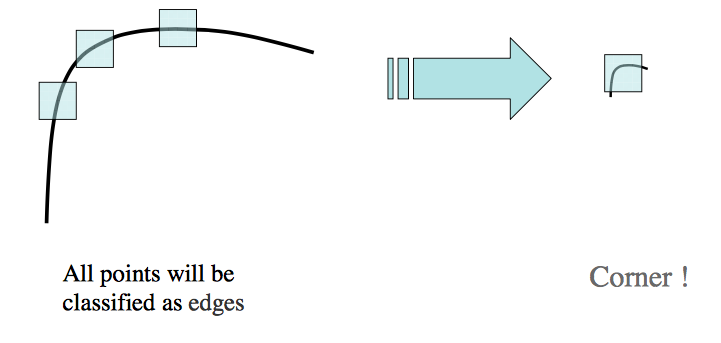
\includegraphics[scale=0.4]{pics/harris_corner}
\caption{Harris is not scale invariant. \label{fig:harris_scale}}
\end{center}
\end{figure}
\item Invariant to \textbf{affine intensity changes}: eigenvalues are scaled by a constant factor but the position of the maxima remains the same.
\end{itemize}
\end{answer}
\item \textit{What is the repeatability of the Harris detector after a rescaling of 2?}
\begin{answer}
\textbf{Repeatability}= $\frac{\# \text{correspondences detected}}{\# \text{correspondences present}}$. 18 $\%$ of the possible correspondences are redetected
\end{answer}
\end{enumerate}

\item \textit{Scale-invariant detection: }
\begin{enumerate}
\item \textit{How does automatic scale selection work? }
\begin{answer}
A possible solution is to rescale the patch (bring it to the canonical scale). A problem with that, is that you have to do it \textbf{individually} for all patches in one image (complexity $(N\cdot M)^2$). $\rightarrow$ We take a local maximum of the function: the region size for which the maximum is achieved, should be invariant to image scale. \textbf{This scale invariant region size is found in each image independently}.
\begin{enumerate}
\item Design a function on the image patch, which is scale invariant, i.e., which has the same value for corresponding regions, even if they are at different scales.
\item For a point in one image, we can consider the average intensity as a function of region size (x-axis). 
\item By comparing the intensity of the \textbf{same feature} in a different scaled image, we can retrieve the scale of the images when the intensity are the \textbf{same}. 
\item  When the right scale is found, the patch must be \textbf{normalized}.
\end{enumerate}
\end{answer}
\item \textit{What are the good and the bad properties that a function for automatic scale selection should have or not have?}
\begin{answer}
\
\begin{itemize}
\item Good function: single and sharp peaks! (LoG)
\item Bad function: flat peak or multiple peaks $\rightarrow$ assign \textbf{more} region sizes to have a unique feature. Blobs and corners are the ideal locations!
\end{itemize}
\end{answer}
\item \textit{How can we implement scale invariant detection efficiently? (show that we can do this by resampling the image vs rescaling the kernel). }
\begin{answer}
\textbf{Rescaling the Kernel}: Convolve image with kernel to identify sharp discontinuities:
\begin{equation}
f=\text{Kernel}*\text{Image}
\end{equation}
It has been shown that the Laplacian of Gaussian kernel is optimal under certain assumptions
\begin{equation}
\text{LoF}=\nabla^2G(x,y)=\frac{\partial G(x,y)}{\partial x^2}+\frac{\partial G(x,y)}{\partial y^2},
\end{equation}
Then, the \textbf{correct scale} is found as local maxima or minima across consecutive smoothed images. This should be done for \textbf{several} region sizes. \\
\textbf{Resampling the Image}: an efficient implementation of multi-scale detection uses the method \textbf{scale-space pyramid}: instead of varying the window size of the feature detector, the idea is to generate upsampled (enlarge the image, interpolating) or downsampled versions of the \textbf{same image}. Then, the \textbf{correct scale} is found as local maxima or minima across consecutive smoothed images. 
\end{answer}
\item \textit{What is the Harris Laplacian and what is its repeatability after a rescaling of 2?}
\begin{answer}
The \textbf{Harris-Laplacian} is a multiscale Harris detector and has a much higher repeatability rate across different scales than the normal Harris detector. After rescaling of 2, the repeatability rate is ca. 65 $\%$.
\end{answer}
\end{enumerate}
\end{enumerate}
\subsection*{Point feature descriptor and matching}
\begin{enumerate}
\item \textit{What is a feature descriptor? (patch of intensity value vs histogram of oriented gradients). How do we match descriptors?}
\begin{answer}
A feature descriptor is an algorithm which takes an image and outputs feature descriptors/feature vectors. Feature descriptors encode interesting information into a series of numbers and act as a sort of numerical \textit{fingerprint} that can be used to differentiate one feature from another.
\begin{itemize}
\item \textbf{Simplest Descriptor}: \textbf{Intensity} values within a squared patch or gradient histogram.
\begin{enumerate}
\item Start with an \textit{empty} canonical patch (all pixels set to 0).
\item For each pixel in the empty patch apply the \textbf{warping function $W(x,y)$} of the corresponding position in the detected image.
\item Interpolate the intensity values of the 4 closest pixels in the detected image using \textit{nearest neighbor} or \textit{bilinear interpolation}
\begin{equation*}
I(x,y)=I(0,0)\cdot (1-x)\cdot (1-y)+I(0,1)\cdot (1-x)\cdot y+I(1,0)\cdot x \cdot (1-y)+I(1,1)\cdot xy.
\end{equation*}
\end{enumerate}
Using the eigenvalues (size) and the eigenvectors (direction) of the \textbf{Harris} detector as \textbf{warp information}, slight view-point invariance can be achieved. \\
Cons: if not warped, very small errors in rotation, scale and view-point will affect matching score significantly, \textbf{computationally expensive}
\item \textbf{Census transform} or \textbf{Histograms of Oriented Gradients (HOG)}.
\begin{enumerate}
\item Compute a histogram of orientations of \textbf{intensity gradients}
\item Peaks in histogram = dominant orientations
\item \textbf{Keypoint orientation = histogram peak}, if there are multiple candidate peaks, construct a different keypoint for each such orientation
\item Rotate patch according to this angle $\rightarrow$ puts the patches into a canonical orientation
\end{enumerate}
\end{itemize}
\begin{figure}[h!]
\begin{center}
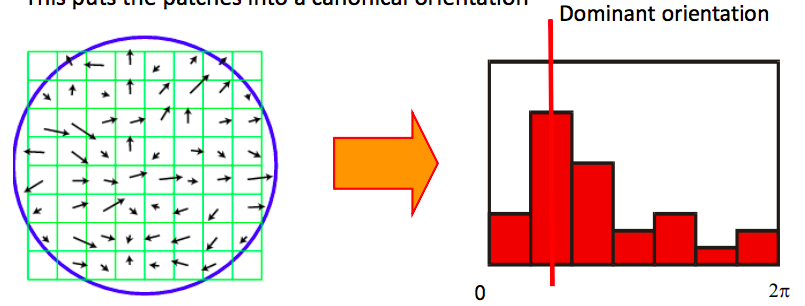
\includegraphics[scale=0.4]{pics/hog}
\caption{Rotation of a patch. Sum up the magnitude of vectors with the same orientation \label{hog}}
\end{center}
\end{figure}
The \textbf{matching} can be done using \textbf{Hamming Distance (Census)} or \textbf{(Z)SSD,(Z)SAD}, \textbf{(Z)NCC}. 
\end{answer}
\item \textit{Scale Invariant Feature Transform detection and descriptor:} 
\begin{enumerate}
 \item \textit{How is the keypoint detection done in SIFT and how does this differ from Harris Laplacian? }
\begin{answer}
The SIFT algorithm:
\begin{itemize}
\item Identification of Keypoint \textbf{location and scale}.
\item Orientation assignment.
\item Generation of keypoint descriptor.
\item Can handle changes in viewpoint (up to 60 degree out-of-plane rotation).
\item Can handle significant changes in illumintation.
\item Computationally expensive.
\end{itemize}
SIFT keypoints are local extrema (maxima and minima) in both \textbf{space and scale} of the DoG images: 
\begin{enumerate}
\item The initial image is \textbf{incrementally convolved with Gaussians} $G(k\sigma)$ to produce images separated by a constant factor $k$ in scale space.
\begin{enumerate}
\item The initial Gaussian $G(\sigma)$ has $\sigma=1.6$.
\item $k$ is chosen such that $k=2^{\frac{1}{s}}$, where $s$ in an integer (typically $s=3$).
\item For efficiency reasons, when $k$ reaches 2, the image is downsampled by a factor of 2 and then the procedure is repeated up to 4 or 6 octaves (pyramid levels).
\end{enumerate}
One image blurred with different strong Gaussian filter $\rightarrow$ shows different level of details
\item Adjacent image scales are then subtracted to produce the difference-of-Gaussian (DoG) images. \\
eg Image(kernel=3)-image(kernel=5) $\rightarrow$ fine details as twigs and hair can be seen\\
 $\uparrow$ kernel $\rightarrow$ larger patches bright and dark spots
\item Detect maxima and minima of Difference-of-Gaussian in scale space.
\item Each point is compared to its 8 neighbors in the current image and 9 neighbors each in the scales above and below.
\item For each max and min found, the output is the location and the scale: this is a candidate keypoint.
\end{enumerate}
Main difference to Harris-Laplacian:\textbf{keypoint location} While in Harris, the keypoint is identified in the image plane as local maximum of the corner function, in SIFT the keypoint is a local minimum or maximum of the DoG image in both position \textbf{and} scale.\\
\end{answer}
\item \textit{How does SIFT achieve orientation invariance? }
\begin{answer}
%from book
The \textbf{descriptor} makes the SIFT robust to rotation, small changes of illumination, scale and viewpoint. Each keypoint is assigned to a specific orientation to make it invariant to image rotation. 
\begin{enumerate}
\item for every pixel around the keypoint, the intensity gradient (mag + orientation) is computed
\item pixel weighted by mag $\rightarrow$ HOG
\item orientation corresponding to the highest peak is assigned to the keypoint
\item all the properties of the keypoint will be measured relative to the keypoint orientation
\end{enumerate}
\end{answer}
\item \textit{How is SIFT descriptor built?}
\begin{answer}
Descriptor computation:
\begin{enumerate}
\item Divide the patch into $4\times4$ sub-patches=16 cells.
\item Compute HOG (8 bins, i.e. 8 directions) for all pixels inside each sub-patch. see Figure \ref{hog}
\item Concatenate all HOGs into a single 1D vector. This is the resulting SIFT descriptor: $4\times 4 \times 8=128$ values.
\item Descriptor matching: SSD (euclidean-distance).
\end{enumerate}
\end{answer}
\item \textit{What is the repeatability of the SIFT detector after a rescaling of 2? }
\begin{answer}
The \textbf{repeatability} can be expressed as
\begin{equation}
\frac{\text{number of correspondences detected}}{\text{number correspondences present}}
\end{equation}
The highest repeatability is obtained when sampling 3 scales per octave.\\
\textbf{Detected} $\sim 90 \%$\\
\textbf{Correctly matched } around 80 $\%$
\end{answer}
\item \textit{ And for a 50 degree viewpoint change?}
\begin{answer}
\textbf{Correctly matched}, location only 73 $\%$, location and orientation 65 $\%$
\end{answer}
\item \textit{Illustrate the 1st to 2nd closest ratio of SIFT detection: what’s the intuitive reasoning behind it?}
\begin{answer}
While brut-force feature \textbf{matching}, issues with closest descriptor can happen. This can give good scores to very ambiguous (bad) matches, due to background clutter or were not detected in the image 1.  The better approach is to compute ration of distances to 1st to 2nd closes match:
\begin{equation}
\frac{d(f_1)}{d(f_2)}<\text{Threshold (usually 0.8)},
\end{equation}
where
\begin{equation}
\begin{split}
d(f_1) &\text{ is the distance of the closest neighbor}\\
d(f_2) &\text{ is the distance of the second closest neighbor}
\end{split}
\end{equation}
Correct matches need to have the closest neighbor significantly closer than the closest incorrect match, to achieve reliable matching. Moreover, for \textbf{false matches}, there will likely be a number of other false matches within similar distances due to the high dimensionality of the feature space. (aka \textbf{curse of dimensionality}). We can think of the second closest match as providing an estimate of the density of false matches within this portion of the feature space, and at the same time identifying specific instances of feature ambiguity.
\end{answer}
\item \textit{Where does the 0.8 threshold come from?}
\begin{answer}
\
\begin{itemize}
\item Eliminates 90\% of the false matches,
\item Discards less than 5\% of the correct matches.
\end{itemize}
\end{answer}
\end{enumerate}
\item \textit{Brief overview of FAST, SURF, BRIEF, ORB and BRISK. Pros and cons of Harris, SIFT, SURF and FAST and BRIEF, ORB and BRISK in terms of localization accuracy, relocalization, and efficiency (see recap table in the slides).}
\begin{answer}
Summary Table \ref{tab:summary} and Figure \ref{recap}.\\
\begin{table}[h!]
\tiny
\begin{tabular}{l | p{7cm} p{3cm}  p{3cm} }
	\hline
	Detector/Descriptor & Brief Overview & Pros & cons\\
	\hline
	Harris detector& corner & rotation invariant & no blob detection, not scale and affine invariant\\
	SIFT both&  blob &rotation, scale and affine invariant & no corner detection, inefficient\\
	SURF both &  Speeded Up Robust Features. Based on ideas similar to SIFT.  blob detector. Approximated computation for detection and descriptor using box filters. & rotation, scale and affine invariant, faster computation, shorter descriptor   & no corner detection, inefficient\\
	FAST detector& Feastures from Accelerated Segment Test. Studies intensity of pixels around candidate pixel $C$. $C$ is FAST corner \textbf{if} a set on $N$ contiguous pixels on circle are all brighter than $intensity(C)+threshold$ or all darker than $intensity(C)+threshold$. & very fast detector& no blob detection, not scale and affine invariant \\
BRIEF descriptor  & Binary Robust Independent Elementary Features. For \textbf{binary} see summary. The \textbf{pattern is generated randomly} (or by ML) only once: then, same pattern is used for all patches. &very fast Hamming distance matching: count the number of bits that are different in the descriptors matched. & not scale or rotation invariant\\
	ORB descriptor& Oriented FAST and Rotated BRIEF. Keypoint detector based on FAST. BRIEF descriptors are steered according to keypoint orientation& binary features are learned by minimizing the correlation on a set of training pathces&\\\setcounter{section}{4}
\setcounter{subsection}{0}\setcounter{section}{4}
\setcounter{subsection}{0}
	BRISK descriptor&Binary Robust Invariant Scalable Keypoints. Detect corners in scale-space using FAST. compare short and long distance pairs for orientation assignment and descriptor formation &rotation and scale invariant, 10 times faster than SURF & \\
	\hline
\end{tabular}
\caption{Summary Descriptor Table\label{tab:summary}}
\end{table}
\begin{figure}[h!]
\begin{center}
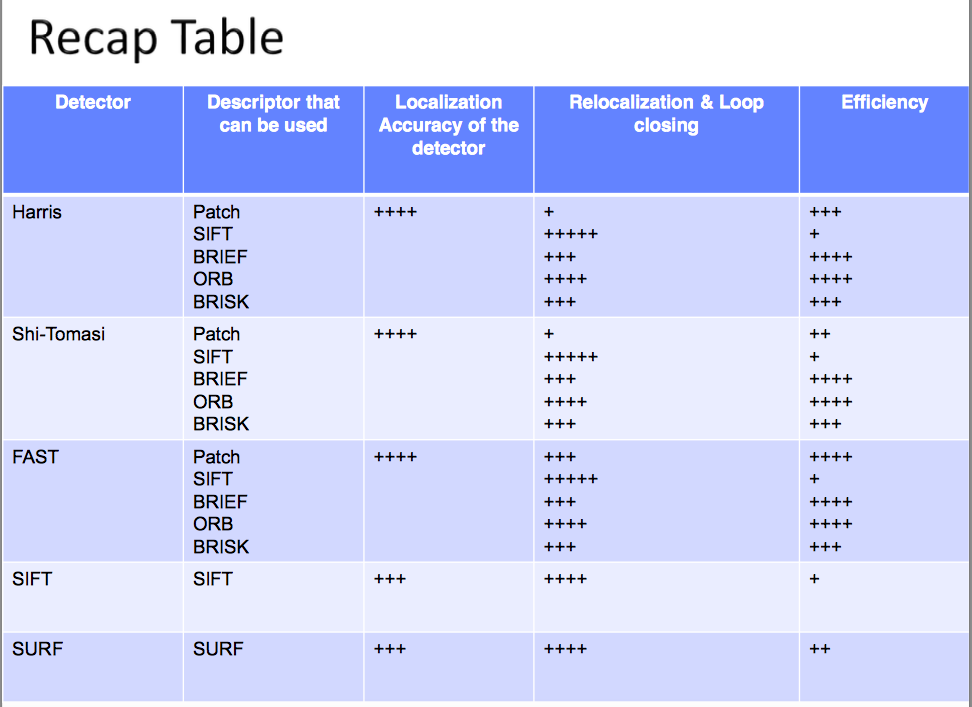
\includegraphics[scale=0.4]{pics/recap}
\caption{Recap for detectors and descriptors \label{recap}}
\end{center}
\end{figure}
\end{answer}
\item \textit{Describe two different ways of tracking features between frames (hint: exercises and VO project)} ????
\begin{answer}
Find a set of likely feature locations in a first image and to then search for their corresponding locations in subsequent images. 
\begin{enumerate}
\item Detect good features which have high eigenvalues in the auto-correlation matrix to provide stable locations at which to find correspondences. Use Harris corner detector 
\item Assign descriptors to the keypoints using HOG
\item Or use SIFT detection and descriptor in step 1. and 2. 
\item In subsequent images, search for locations where the corresponding descriptor has low SSD.
\end{enumerate}
\end{answer}
\end{enumerate}
\newpage
\section*{Lecture 07 Multiple view geometry 1}
\begin{enumerate}
\item \textit{SFM vs 3D reconstruction: definition.}
\begin{answer}
\
\begin{itemize}
\item \textbf{3D reconstruction from multiple views}
\begin{itemize}
\item \textbf{Assumption:} $K,T,R$ are \textbf{known}.
\item \textbf{Goal:} Recover the 3D structure from images.
\end{itemize}
\item \textbf{Structure from motion}
\begin{itemize}
\item \textbf{Assumption:} $K,T,R$ are \textbf{unknown}.
\item \textbf{Goal:} Recover simultaneously 3D scene structure and camera poses (up to scale) from multiple images.
\end{itemize}
\end{itemize}
\end{answer}
\item \textit{Stereo vision}:
\begin{enumerate}
\item \textit{Definition of disparity. Simplified case and general case}
\begin{answer}
Disparity means a great difference. Stereopsis is a term that is most often used to refer to the perception of depth and 3-dimensional structure obtained on the basis of visual information of a left and a right image.  $\rightarrow$ Stereo Vision\\
The basic principle behind stereo vision is \textbf{triangulation}.
\begin{itemize}
\item Gives reconstruction as intersection of two rays.
\item Requires \textbf{camera pose (calibration) and point correspondence} (matching pairing points of the two images which are the projection of the same point in the scene).
\end{itemize}
There are basically two cases
\begin{enumerate}
\item Simplified case: identical cameras are \textbf{aligned}. The two cameras are identical, meaning that they have the same \textbf{focal length}, and are \textbf{aligned} with the $x$-axis. 
\item General case: different cameras are \textbf{not aligned}. Two identical cameras do not exist in nature! Aligning both cameras on a horizontal axis is very hard. in order to use a stereo camera $\rightarrow$ Find Extrinsic $(R,t)$ and Intrinsic $(f,C,radial distortion)$ parameters. $\rightarrow$ camera calibration (Tsai or Homographies)
\end{enumerate}
\begin{figure}[ht]
\begin{center}
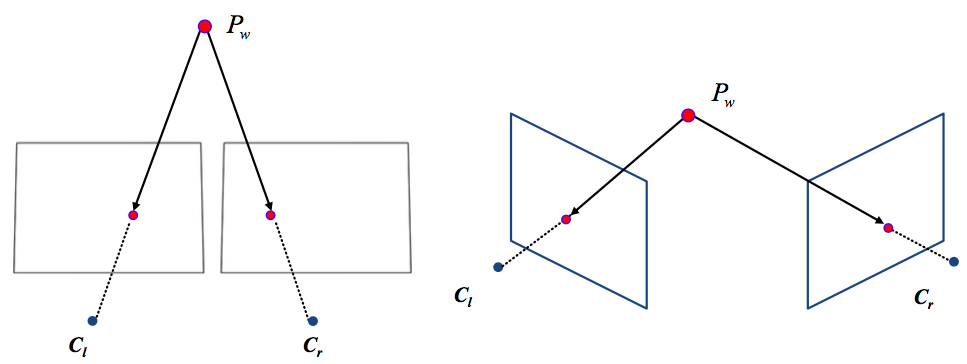
\includegraphics[scale=0.4]{pics/stereo_vision}
\caption{Simplified case and General case\label{stereo vision}}
\end{center}
\end{figure}
\end{answer}

\item \textit{Mathematical expression of depth as a function of baseline, disparity and focal length?}

\begin{minipage}{0.3 \columnwidth}
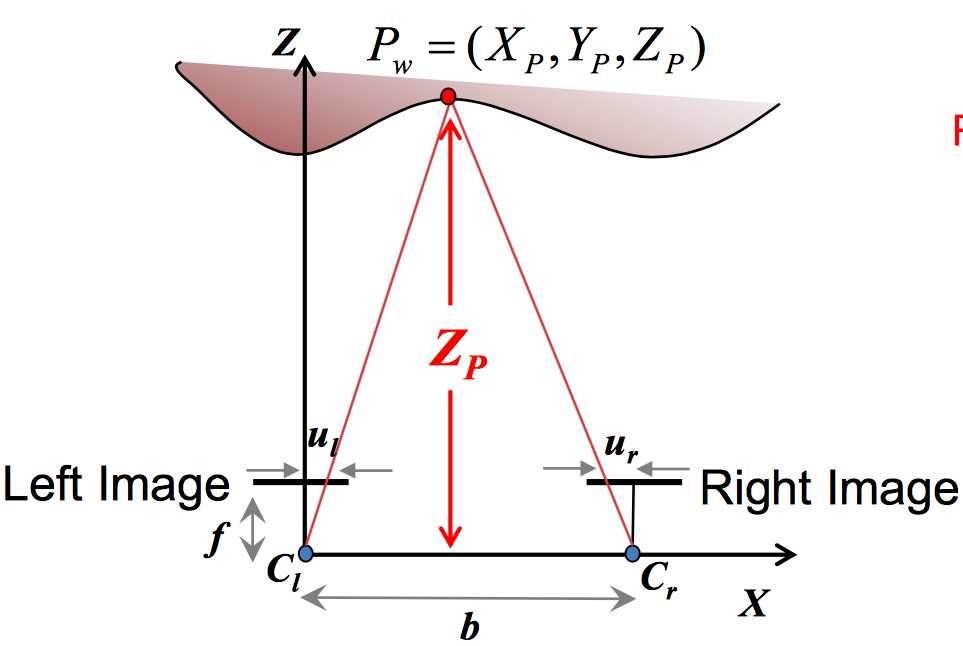
\includegraphics[width=\textwidth]{pics/stereo_vis}
\tiny{Simple Case of Stereo Vision}\label{setero_vis}
\end{minipage}
\hfill
\begin{minipage}{0.6 \columnwidth}
If we have a world point $P_w$, a distance from the axis to the point $Z_P$, a distance between the cameras $b$, focal length $f$ and pixel coordinates from the corresponding world points $u,v$, we can use similar triangles from Figure \ref{setero_vis} and get
\begin{equation}
\begin{split}
\frac{f}{Z_P}&=\frac{u_l}{X_P}\\
\frac{f}{Z_P}&=\frac{-u_r}{b-X_P}\\
\end{split}
\Rightarrow X_P=\frac{u_l\cdot b}{u_l-u_r}
\Rightarrow Z_P=\frac{b\cdot f}{u_l-u_r}.
\end{equation}
\end{minipage}
Observation from this equation are
\begin{itemize}
\item Distance $Z_P$ is inversely proportional to \textbf{disparity}: the distance to near objects can be measured more accurately than that to distant objects.
\item \textbf{Disparity}: $u_l-u_r$ and proportional to $b$.  For a given disparity error, the accuracy of depth estimate increases with increasing baseline $b$. increasing disparity with the distance of the objects from the fixation point 
\item As $b$ is increased, since the distance of the two cameras is increased, some objects may appear in one camera but not in the other (field of view of cameras). These objects won't have disparity.
\item If the\textbf{ baseline} $b$ is unknown it is possible to reconstruct the scene up to a scale (structure from motion!) 
\end{itemize}
\item \textit{Apply error propagation to derive expression of depth uncertainty. How can we improve the uncertainty?}
\begin{answer}
\begin{equation}
Z_P=\frac{b\cdot f}{u_l-u_r} \rightarrow \sigma_{depth}= \sqrt{(\frac{\partial Z_p}{\partial b})^2 \sigma_b^2+ (\frac{\partial Z_p}{\partial f})^2 \sigma_f^2 + (\frac{\partial Z_p}{\partial u_l})^2 \sigma_{ul}^2 + (\frac{\partial Z_p}{\partial u_r})^2 \sigma_{ur}^2}
\end{equation}
Increase baseline or focus.  Decrease depth, $u_l$ or $u_r$
\end{answer}
\item \textit{Large baseline vs small baseline. }
\begin{answer}
\
\begin{itemize}
\item \textbf{Too small:}
\begin{itemize}
\item Large depth error
\item Quantification of error as a function of the disparity?
\end{itemize}
\item \textbf{Too large:}
\begin{itemize}
\item Minimum measurable distance increases.
\item Difficult search problem for close objects.
\end{itemize}
\end{itemize}
\end{answer}
\item \textit{What is the closest depth a stereo camera can measure? Can you derive it mathematically?}
\begin{answer}
In a simplified case, $u_l = \text{image width}/2$, $u_r=- \text{image widht}/2$,   where the depth $Z_P=\underbrace{\frac{b\cdot f}{u_l-u_r} }_{\uparrow}\quad \rightarrow \downarrow Z_P  $
\end{answer}
\item \textit{Stereo vision general case: show mathematically how we can compute the intersection of two lines, both linearly and non linearly. }
\begin{answer}
 Lines do not always intersect in the 3D space: we want to minimize the error. For the two cameras we have
\begin{equation}
\tilde{p}_l=\lambda_l\cdot \begin{pmatrix}
 u_l\\
 v_l\\
 1
 \end{pmatrix}=K_l\cdot \begin{pmatrix}
 X_w\\
 Y_w\\
 Z_w
 \end{pmatrix}, \quad \tilde{p}_r=\lambda_r\cdot \begin{pmatrix}
 u_r\\
 v_r\\
 1
 \end{pmatrix}=K_r\cdot R\cdot \begin{pmatrix}
 X_w\\
 Y_w\\
 Z_w
 \end{pmatrix}+T. 
\end{equation}
\textbf{Triangulation:} The problem of determining the 3D position of a point given a set of corresponding image locations and known camera poses.\\ In order to triangulate, we use \textbf{least-squares} approximation:
\begin{equation}
\begin{split}
\lambda_1\cdot \begin{pmatrix}
 u_1\\
 v_1\\
 1
 \end{pmatrix}=K\cdot [I|0]\cdot \begin{pmatrix}
 X_w\\
 Y_w\\
 Z_w\\
 1
 \end{pmatrix}&\Rightarrow \lambda_1p_1=M_1\cdot P \qquad \text{left camera}. \\
 \lambda_2\cdot \begin{pmatrix}
 u_2\\
 v_2\\
 1
 \end{pmatrix}=K\cdot [R|T]\cdot \begin{pmatrix}
 X_w\\
 Y_w\\
 Z_w\\
 1
 \end{pmatrix}&\Rightarrow \lambda_2p_2=M_2\cdot P \qquad \text{right camera}.
\end{split}
\end{equation}
\textbf{Triangulation: least-squares approximation}
We solve for $P$ and get a system $A\cdot \begin{pmatrix} \lambda_1 \\\lambda_2 \end{pmatrix}=b$, which cannot be inverted (A is $3\times 2$). We use pseudoinverse approximation (least squares) and get
\begin{equation}
A^T\cdot A\cdot \begin{pmatrix}
 \lambda_1\\
 \lambda_2
 \end{pmatrix}=A^T\cdot b \Rightarrow \begin{pmatrix}
 \lambda_1\\
 \lambda_2
 \end{pmatrix}=(A^T\cdot A)^{-1}\cdot A^T\cdot b.
\end{equation}
\begin{bmk}
This is a problem with 6 equations and 5 unknowns: the 3 element of the coordinates of the world point and the two depth factors $\lambda_1,\lambda_2$.
\end{bmk}

\textbf{Triangulation: Nonlinear approach}: 
We want to find $P$ that minimizes the \textbf{sum of squared reprojection error}
\begin{equation}
SSRE=d^2(p_1,\pi_1(P))+d^2(p_2,\pi_2(P)),
\end{equation}
where 
\begin{equation}
d(p_1,\pi_1(P))=||p_1-\pi_1(P)||
\end{equation}
is called \textbf{reprojection error}. The observed point is $p_1,p_2$ and the reprojected one is $M_1P,M_2P$. In practice, this is done by initializing $P$ using linear approach and then minimize SSRE using Gauss-Newton of Levenberg-Marquardt.
\end{answer}
\item \textit{What is the geometric interpretation of the linear and non linear approaches and what error term do they minimize? (write it mathematically). }
\begin{answer}
\textbf{Geometric Interpretation}:  
Given the projections $p_{1,2}$ of a 3D point $P$ in two or more images, we want to find the coordinates of the 3D point by intersecting the two rays corresponding to the projections. We want to find the shortest segment connecting the two viewing rays and let $P$ be the \textbf{midpoint} of the segment. The two rays won't meet exactly because of \textbf{noise} and \textbf{numerical errors}.\\
\textbf{Reprojection error}
\begin{equation}
d(p_1,\pi_1(P))=||p_1-\pi_1(P)||
\end{equation}

\end{answer}
\item \textit{Correspondence problem: epipolar geometry; definition of epipole, epipolar line, and epipolar plane.}
\begin{answer}
Given a point $p$ in a first image, where is its corresponding point $p'$ in the right image? \\
\textbf{Correspondence Search}: Identify image patches in the left and in the right images, corresponding to the same scene structure. Similarity measures:
\begin{itemize}
\item (Z)ZNCC
\item (Z)SSD
\item (Z)SAD
\item Census Transform
\end{itemize}
To make the search less computationally expensive, search in 1D. Potential matches for $p$ \textbf{have to lie} on the corresponding epipolar line $l'$.
\begin{itemize}
\item \textbf{epipole} is the projection of the optical center on the other camera image.
\item \textbf{epipolar line} is the projection of the infinite ray $\pi^{-1}(p)$ corresponding to $p$ in the other camera image. Since $\pi(p)=\lambda K$, $\pi(p)^{-1}=\lambda K^{-1}p$. This makes sense: if we observe a projection $p_1$ in the left camera, this can correspond to each world point lying on the infinite ray (every one of these points would project into $p_1$). All these points have a different projection on the right camera, which in 2D forms the epipolar line.
\item \textbf{epipolar plane} is uniquely defined by the two optical centers $C_l$, $C_r$ and one image point \textit{p}
\end{itemize}
\begin{figure}[h!]
\begin{center}
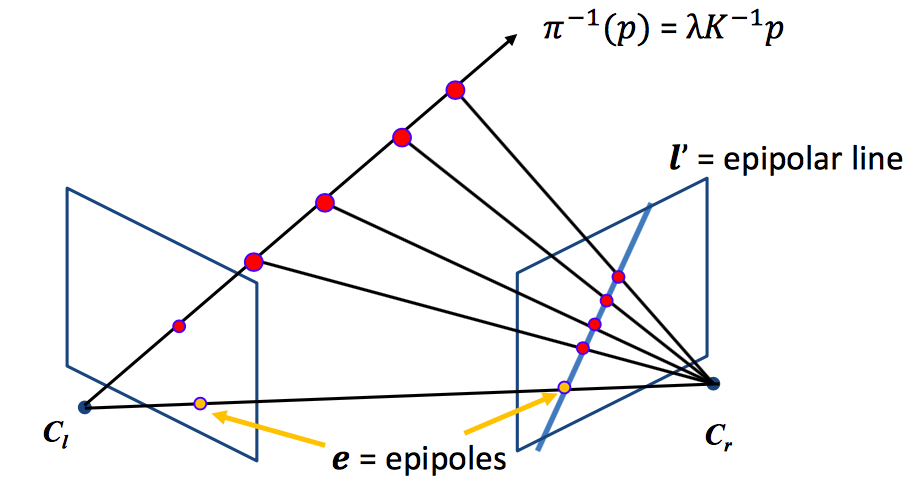
\includegraphics[scale=0.4]{pics/epi}
\caption{Epipolar lines and epipoles. \label{fig:epi}}
\end{center}
\end{figure}
\end{answer}
\item \textit{Draw epipolar lines for two converging cameras, for a forward moving camera, for a side-moving camera.} 
\begin{answer}
\textbf{Convergence Plane} is where the focus of two cameras meet / attention of screen.  
\begin{itemize}
\item \textbf{Two converging cameras:} see Figure \ref{fig:epi} tilted. All epipolar lines intersect at the epipole! As the position of the 3D point varies, the epipolar line \textit{rotates} about the baseline. 
\item  Forward moving camera the line are radiating from the epipolar point. in both images the coordinates of the epipolar point is the \textbf{same}
\item Side-moving camera the line is horizontal and the epipolar point is at infinity
\end{itemize}
\end{answer}
\end{enumerate}

\item \textit{Stereo rectification and mathematical derivation of rectifying homographies.}
\begin{answer}
Stereo rectification waprs left and right images into new rectified images, whose epipolar lines are aligned to the baseline.\\
\textbf{Goal:} make correspondence search simpler and more efficient, because search is done along the horizontal line of the recitified images.
\begin{enumerate}
\item compute homographies for each imput image reprojection
\item project image planes onto a common plane parallel to the baseline
\item epipolar lines are horizontal and the scanlines of the left and right image are aligned
\end{enumerate}
Mathematical derivation 
\begin{enumerate}
\item The perspective equation for a point in the world is 
\begin{equation}
\text{image point}=\tilde{p}=\begin{pmatrix}
\tilde{u}\\
\tilde{v}\\
\tilde{w}
\end{pmatrix} = \lambda \begin{pmatrix}
 u\\
 v\\
 1
 \end{pmatrix}=K[R|T]\cdot \begin{pmatrix}
 X_w\\
 Y_w\\
 Z_w\\
 1
 \end{pmatrix}.
 \end{equation}
This can be rewritten in a more convenient way by considering $[R|T]$ as the transformation from the world to the Camera frame ($T$ expressed as $C$):
\begin{equation}
 \lambda \begin{pmatrix}
 u\\
 v\\
 1
 \end{pmatrix}=K\cdot R^{-1}\cdot \left(\begin{pmatrix}
 X_w\\
 Y_w\\
 Z_w
 \end{pmatrix}-C\right)
\end{equation}
\item We can then write the Perspective Equation for the Left and Right cameras: we assume for generality that they have the same intrinsic parameters:
\begin{equation}
\begin{split}
\lambda_L\cdot \begin{pmatrix}
 u_L\\
 v_L\\
 1
 \end{pmatrix}&= K_L\cdot R_L^{-1}\cdot \left(\begin{pmatrix}
 X_w\\
 Y_w\\
 Z_w
 \end{pmatrix}-C_L\right) \quad \text{left camera}\\
 \lambda_R\cdot \begin{pmatrix}
 u_R\\
 v_R\\
 1
 \end{pmatrix}&= K_R\cdot R_R^{-1}\cdot \left(\begin{pmatrix}
 X_w\\
 Y_w\\
 Z_w
 \end{pmatrix}-C_R\right) \quad \text{right camera}
\end{split}
\end{equation}
\item The goal of stereo rectification is to warp left and right camera images such that their focal planes are \textbf{coplanar} and the intrinsic parameters are identical. It follows 
\begin{equation}
\begin{split}
\lambda_L\cdot \begin{pmatrix}
 u_L\\
 v_L\\
 1
 \end{pmatrix}&= K_L\cdot R_L^{-1}\cdot \left(\begin{pmatrix}
 X_w\\
 Y_w\\
 Z_w
 \end{pmatrix}-C_L\right) \rightarrow \overline{\lambda}_L\cdot \begin{pmatrix}
 \overline{u}_L\\
 \overline{v}_L\\
 1
 \end{pmatrix}= \overline{K}\cdot \overline{R}^{-1}\cdot \left(\begin{pmatrix}
 X_w\\
 Y_w\\
 Z_w
 \end{pmatrix}-C_L\right) \\
 \lambda_R\cdot \begin{pmatrix}
 u_R\\
 v_R\\
 1
 \end{pmatrix}&= K_R\cdot R_R^{-1}\cdot \left(\begin{pmatrix}
 X_w\\
 Y_w\\
 Z_w
 \end{pmatrix}-C_R\right) \rightarrow \overline{\lambda}_R\cdot \begin{pmatrix}
 \overline{u}_R\\
 \overline{v}_R\\
 1
 \end{pmatrix}= \overline{K}\cdot \overline{R}^{-1}\cdot \left(\begin{pmatrix}
 X_w\\
 Y_w\\
 Z_w
 \end{pmatrix}-C_R\right) 
\end{split}
\end{equation}
\item By solving for $\begin{pmatrix}
 X_w\\
 Y_w\\
 Z_w \end{pmatrix}$ for each camera, we can compute the Homography (or warping) that needs to be applied to rectify each camera image:
\begin{equation}
\begin{split}
\overline{\lambda}_L\cdot \begin{pmatrix}
 \overline{u}_L\\
 \overline{v}_L\\
 1
 \end{pmatrix}&=\lambda_L \cdot \underbrace{\overline{K}\cdot \overline{R}^{-1} \cdot R_L \cdot K_L^{-1}}_{\text{homography left camera}} \cdot \begin{pmatrix}
 u_L\\
 v_L\\
 1
 \end{pmatrix}\\
 \overline{\lambda}_R\cdot \begin{pmatrix}
 \overline{u}_R\\
 \overline{v}_R\\
 1
 \end{pmatrix}&=\lambda_R \cdot \underbrace{\overline{K}\cdot \overline{R}^{-1} \cdot R_R \cdot K_R^{-1}}_{\text{homography right camera}} \cdot \begin{pmatrix}
 u_R\\
 v_R\\
 1
 \end{pmatrix}
\end{split}
\end{equation}
\item The new $\overline{K},\overline{R}$ can be chosen as
\begin{equation}
\begin{split}
\overline{K}&=\frac{K_L+K_R}{2}\\
\overline{R}&=[\overline{r}_1,\overline{r}_2,\overline{r}_3],
\end{split}
\end{equation}
where $\overline{r}_1,\overline{r}_2,\overline{r}_3$ are the column vectors of $\overline{R}$. These can be computed as
\begin{equation}
\begin{split}
\overline{r}_1&=\frac{C_2-C_1}{||C_2-C_1||}\\
\overline{r}_2&=r_3 \times \overline{r_1} \text{ where } r_3 \text{ is the third column of }R_L\\
\overline{r}_3&=\overline{r}_1\times \overline{r}_2.
\end{split}
\end{equation}
For more details have a look at \textit{A compact alg. for rectification of stereo pairs}.
\end{enumerate}
\begin{minipage}{0.6 \columnwidth}
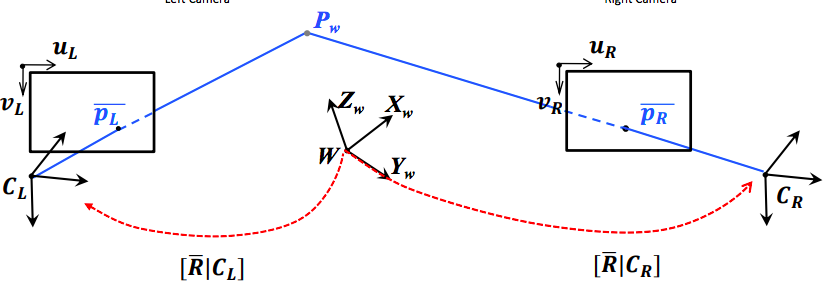
\includegraphics[width=\textwidth]{pics/rectif2}\label{fig:rectif2}
\end{minipage}
\hfill
\begin{minipage}{0.3 \columnwidth}
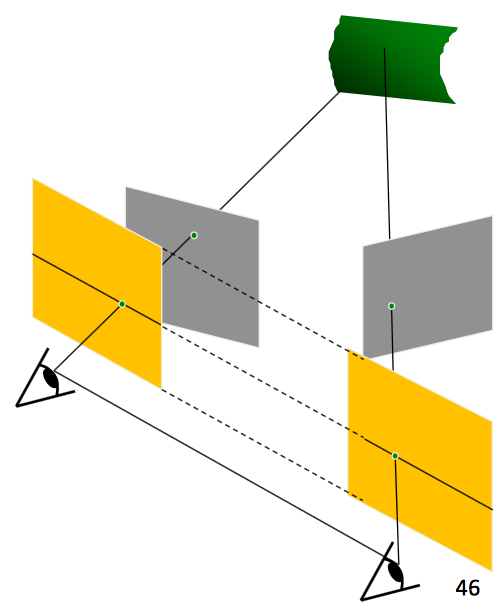
\includegraphics[width=0.8\textwidth]{pics/rectif}\label{fig:rectif}
\end{minipage}

\end{answer}
\item \textit{Disparity map. How is it computed?}
\begin{answer}
A disparity map appear as a grayscale image where the intensity of every pixel point is proportional to the disparity of that pixel in the left and right image: objects that are closer to the camera appear lighter, while farther objects appear darker.
Input to dense 3D reconstruction
\begin{enumerate}
\item For each pixel in the left image, find its corresponding point in the right image.
\item Compute the disparity for each pair of correspondences.
\item Visualized in gray-scale or color coded image.
\end{enumerate}
Close objects experience bigger disparity. They appear brighter in disparity map.
The depth $Z$ can be computed from the disparity by recalling that
\begin{equation}
Z_P=\frac{bf}{u_l-u_r}
\end{equation}
This is really useful for obstacle avoidance.
Challenges include: occlusion, repetition, non-lambertian surfaces (specularities), textureless surfaces. This is important for obstacle avoidance.
\end{answer}
\item \textit{How to establish stereo correspondences with subpixel accuracy?}
\begin{answer}
From slides and Szeliski book , 
\begin{itemize}
\item To average noise effect, use a window around the point of interest
\item Neighborhoods of corresponding points are similar in intensity patterns(NCC, SSD etc.)
\item Occluded areas can be detected using cross-checking, i.e., comparing left-to- right and right-to-left disparity maps.
\item Associate confidences with per-pixel depth estimates, which can be done by looking at the curvature of the correlation surface, i.e., how strong the minimum in the DSI image is at the winning disparity. $\uparrow$ confidence $\propto$ strong texture 
\end{itemize}

\end{answer}
\item \textit{Describe one or more simple ways to reject outliers in stereo correspondences.}
\begin{answer}
 A median filter can be applied to clean up spurious mismatches, and holes due to occlusion can be filled by surface fitting or by distributing neighboring disparity estimates
 \begin{itemize}
\item Uniqueness: only one match in right image for every point in left image.
\item Ordering: points on same surface will be in same order in both views
\item Disparity gradient: disparity changes smoothly between points on the same surface.
\end{itemize}
\end{answer}
\item \textit{Is Stereo Vision the only way of estimating depth information? If not, list alternative options.}
\begin{answer}
\
\begin{itemize}
\item \textbf{Graph Cuts:} is formulated in terms of energy minimization. solving a maximum flow problem in a graph
\item \textbf{Ground Truth:} information provided by direct observation
\end{itemize}
\end{answer}
\end{enumerate}
\newpage
\section*{Lecture 08/09 Multiple view geometry 2 and 3}
 
\begin{enumerate}
\item \textit{What’s the minimum number of correspondences required for calibrated SFM and why?}
\begin{answer}
In \textit{stereo vision}, only \textbf{5 degrees of freedom} are measurable. The camera relative pose is unknown: this is e.g. the case when the two images are taken from the same camera but at different times and positions.\\
\textbf{Problem formulation:} Given $n$ point correspondences between two images, $\{p_1^i=(u_1^i,v_1^i), \ p_2^i=(u_2^i,v_2^i)\}$, simultaneously estimate the 3D points $P^i$, the camera relative-motion parameters ($R,T$), and the camera intrinsics $K_1,K_2$ that satisfy:
\begin{equation}
\begin{split}
\lambda_1 \cdot \begin{pmatrix}
 u_1^i\\
 v_1^i\\
 1
 \end{pmatrix}&=K_1\cdot [I|0]\cdot \begin{pmatrix}
 X_w^i\\
 Y_w^i\\
 Z_w^i\\
 1
 \end{pmatrix},\\
 \lambda_2 \cdot \begin{pmatrix}
 u_2^i\\
 v_2^i\\
 1
 \end{pmatrix}&=K_2\cdot [R|T]\cdot \begin{pmatrix}
 X_w^i\\
 Y_w^i\\
 Z_w^i\\
 1
 \end{pmatrix}
\end{split}
\end{equation}
We have two cases then:
\subsubsection*{Calibrated Cameras ($K_1,K_2$ known)}
For convenience, we use \textit{normalized image coordinates}
\begin{equation}
\begin{pmatrix}
\bar{u}\\
\bar{v}\\
1
\end{pmatrix}=K^{-1}\cdot \begin{pmatrix}
u\\
v\\
1
\end{pmatrix}.
\end{equation}
We want to find $R,T,P^i$ which satisfy
\begin{equation}
\begin{split}
\lambda_1 \cdot \begin{pmatrix}
 \bar{u}_1^i\\
 \bar{v}_1^i\\
 1
 \end{pmatrix}&=K_1\cdot [I|0]\cdot \begin{pmatrix}
 X_w^i\\
 Y_w^i\\
 Z_w^i\\
 1
 \end{pmatrix},\\
 \lambda_2 \cdot \begin{pmatrix}
 \bar{u}_2^i\\
 \bar{v}_2^i\\
 1
 \end{pmatrix}&=K_2\cdot [R|T]\cdot \begin{pmatrix}
 X_w^i\\
 Y_w^i\\
 Z_w^i\\
 1
 \end{pmatrix}.
\end{split}
\end{equation}
\textbf{Scale Ambiguity}: If we rescale the entire scene by a constant factor (i.e. similarity transformation), the projections (in pixels) of the scene points in both images remain the \textbf{same} (because the angles remain the same).
\begin{itemize}
\item In \textit{monocular} vision it is \textbf{not possible} to recover the absolute scale of the scene.
\item In \textit{stereo vision}, only \textbf{5 degrees of freedom} are measurable:
\begin{itemize}
\item 3 parameters to describe the \textbf{rotation}.
\item 2 parameters for the \textbf{translation up to a scale} (we can only compute the direction of translation but not its length (magnitude)).
\end{itemize}
\end{itemize}
How many knowns and unknowns?
\begin{itemize}
\item $4n$ knowns: $n$ correspondences, each one $(u_1^i,v_1^i)$ and $(u_2^i,v_2^i)$, $i=1,\hdots,n$.
\item $5+3n$ unknowns: 5 for the motion up to a scale (3 rotation and 2 translation) and $3n$ which is the number of coordinates of the $n$ 3D points.
\end{itemize}
It should hold
\begin{equation}
\begin{split}
4n &\geq 5+3n\\
\Rightarrow n&\geq 5.
\end{split}
\end{equation}
\end{answer}
\item \textit{Derive the epipolar constraint.}
\begin{answer}
\begin{equation}
\bar{p}_1=\begin{pmatrix}
\bar{u}_1\\
\bar{v}_1\\
1
\end{pmatrix},\quad \bar{p}_2=\begin{pmatrix}
\bar{u}_2\\
\bar{v}_2\\
1
\end{pmatrix}
\end{equation}
We can observe that $p_1,p_2,T$ are coplanar:
\begin{equation}
\begin{multlined}
p_2^T\cdot n=0 \quad
 \rightarrow  \quad p_2^T\cdot (T\times p_1')=0\quad
 \rightarrow  \quad  p_2^T \cdot (T\times (Rp_1)) =0 \\
 \rightarrow  \quad 
p_2^T\cdot [T]_x\cdot Rp_1 =0 \quad
 \rightarrow  \quad 
p_2^T \cdot E \cdot p_1=0\\
 \text{ is the epipolar constraint, where }E=[T]_x\cdot R \text{ is the essential matrix}. 
 \end{multlined}
\end{equation}
\begin{figure}[h!]
\begin{center}
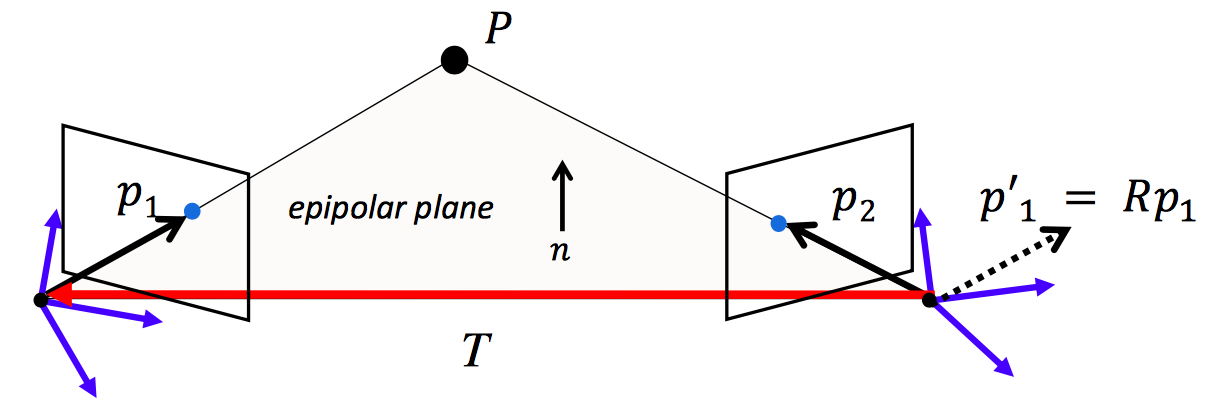
\includegraphics[scale=0.3]{pics/epi_2}
\caption{Epipolar Constraint. \label{fig:epi}}
\end{center}
\end{figure}
\end{answer}
\item \textit{Definition of Essential matrix. }
\begin{answer}
Essential matrix \textbf{E} is a \texttt{3x3} matrix which maps a point $p_1$ from image 1 onto a line $l_2= E p_1$ in image 2  , since $p_2^T l_1 = 0 $\\
\begin{equation}
p_2^T \cdot E \cdot p_1=0
\end{equation}
\textbf{Skew-symmetric matrix of a} 
\begin{equation}
a\times b = \begin{pmatrix}
 0&-a_z&a_y\\
 a_z&0&-a_x\\
 -a_y&a_x&0
 \end{pmatrix}\cdot \begin{pmatrix}
 b_x\\
 b_y\\
 b_z
 \end{pmatrix}=[a]_x\cdot b
\end{equation}
\end{answer}
\item \textit{The 8-point algorithm (derivation).}
\begin{answer}
Starting from \begin{equation}
p_2^T \cdot E \cdot p_1=0
\end{equation},
each pair of point correspondences provides a linear equation. For $n$ points we can write
\begin{equation}
\underbrace{\begin{pmatrix}
\bar{u}_2^1\cdot \bar{u}_1^1&\bar{u}_2^1\cdot \bar{v}_1^1&\bar{u}_2^1&\bar{v}_2^1\cdot \bar{u}_1^1&\bar{v}_2^1\cdot \bar{v}_1^1&\bar{v}_2^1&\bar{u}_1^1&\bar{v}_1^1&1\\
\bar{u}_2^2\cdot \bar{u}_1^2&\bar{u}_2^2\cdot \bar{v}_1^2&\bar{u}_2^2&\bar{v}_2^2\cdot \bar{u}_1^2&\bar{v}_2^2\cdot \bar{v}_1^2&\bar{v}_2^2&\bar{u}_1^2&\bar{v}_1^2&1\\
\vdots &\vdots &\vdots &\vdots &\vdots &\vdots &\vdots &\vdots &\vdots \\
\bar{u}_2^n\cdot \bar{u}_1^n&\bar{u}_2^n\cdot \bar{v}_1^n&\bar{u}_2^n&\bar{v}_2^n\cdot \bar{u}_1^n&\bar{v}_2^n\cdot \bar{v}_1^n&\bar{v}_2^n&\bar{u}_1^n&\bar{v}_1^n&1
\end{pmatrix}}_{Q \text{ (known) }}\cdot  \underbrace{\begin{pmatrix}
e_{11}\\
e_{12}\\
e_{13}\\
e_{21}\\
e_{22}\\
e_{23}\\
e_{31}\\
e_{32}\\
e_{33}\\
 \end{pmatrix}}_{\bar{E} \text{ unknown }}=0
\end{equation}
This problem can be written as
\begin{equation}
Q\cdot \bar{E}=0.
\end{equation}
Two types of solution
\begin{itemize}
\item \textbf{Minimal Solution}
\begin{itemize}
\item $Q_{n\times 9}$ should have rank $8$ to have unique (up to scale) non trivial solution $\bar{E}$.
\item Each point correspondence provides 1 independent equation.
\item Thus, 8 point correspondences are needed.
\end{itemize}
\item \textbf{Over-determined Solution}
\begin{itemize}
\item $n>8$ points.
\item A solution is to minimize $||Q\cdot \bar{E}||^2$ subject to the constraint $||\bar{E}||^2=1$. The solution is the eigenvector corresponding to the smallest eigenvalue of matrix $Q^T\cdot Q$.
\item This can be solved with Singular Value Decomposition = $[U,E,V]$. Last column of the  V $\rightarrow$ E $\rightarrow$ reshape(E)
\end{itemize}
\item \textbf{Degenerate Solution} if 3D points are coplanar. There is the 5 point algorithm which holds also for coplanar points.
\end{itemize}
\end{answer}
\item \textit{How many rotation and translation combinations can the essential be decomposed in?}
\begin{answer}
4, but only one solution where points are in front of both cameras. A valid R has $det(R) = 1$. Ff not, invert the sign of the matrix.
\end{answer}

\item \textit{Geometric interpretation of the epipolar constraint.}
\begin{answer}
If the epipolar constraint
\begin{equation}
p_2^T \cdot E \cdot p_1\neq 0 
\end{equation}
It means that the projection from $p_1$ is not \textit{orthogonal} to $p_2  $. Hence,
\begin{equation}
\bar{p}_2^T\cdot E \cdot \bar{p}_1 = ||\bar{p}_2||\cdot ||E\cdot \bar{p}_1||\cdot \cos(\theta)
\end{equation}
which is not zero is $p_1,p_2,T$ are not co-planar and $\theta\neq 90$. 
\end{answer}
\item \textit{Relation between Essential and Fundamental matrix. }
\begin{answer}
If the cameras are \textbf{uncalibrated} $\Rightarrow$ $K_1$, $K_2$ are unknown.\\
Assumption, Intrinsic parameters are known. It holds 
\begin{equation}
\bar{p}_2^T\cdot E \cdot \bar{p}_1=0,
\end{equation}
where 
\begin{equation}
\begin{pmatrix}
\bar{u}_1^i\\
\bar{v}_1^i\\
1
\end{pmatrix}=K_1^{-1}\cdot \begin{pmatrix}
u_1^i\\
v_1^i\\
1
\end{pmatrix},\quad \begin{pmatrix}
\bar{u}_2^i\\
\bar{v}_2^i\\
1
\end{pmatrix}=K_2^{-1}\cdot \begin{pmatrix}
u_2^i\\
v_2^i\\
1
\end{pmatrix}.
\end{equation}
By rewriting the constraint, one obtains
\begin{equation}
\begin{split}
\begin{pmatrix}
u_2^i\\
v_2^i\\
1
\end{pmatrix}^T\cdot K_2^{-T}\cdot E \cdot K_1^{-1}\cdot \begin{pmatrix}
u_1^i\\
v_1^i\\
1
\end{pmatrix}&=0\\
\begin{pmatrix}
u_2^i\\
v_2^i\\
1
\end{pmatrix}^{T}\cdot F \cdot \begin{pmatrix}
u_1^i\\
v_1^i\\
1
\end{pmatrix}&=0,
\end{split}
\end{equation}
where $F$ is the \textbf{fundamental matrix}, which can be computed as
\begin{equation}
F=K_2^{-T}\cdot E \cdot K_1^{-1}=K_2^{-T}\cdot [T]_x\cdot R \cdot K_1^{-1}.
\end{equation}
\end{answer}
\item \textit{Why is it important to normalize the point coordinates in the 8-point algorithm? Describe one or more possible ways to achieve this normalization.}
\begin{answer}
In case the camera is uncalibrated, matrix Q of equation $Q\cdot F = 0$ contains  orders of magnitudes difference between columns. $\rightarrow$ least-squares yields poor results. $\rightarrow$ Poor numerical conditioning, which makes results very sensitive to noise.\\

\end{answer}
\item \textit{Normalized 8-point algorithm.}
\begin{answer}
This estimates the Fundamental matrix on a set of \textbf{Normalized correspondences} (with better numerical properties) and then \textbf{unnormalizes} the result to obtain the fundamental matrix for the original given correspondences. \\
\textbf{Idea:} Transform image coordinates so that they are in the range $[-1,1]\times [-1,1]$. One way is to apply the following rescaling and shift
\begin{figure}[h!]
\begin{center}
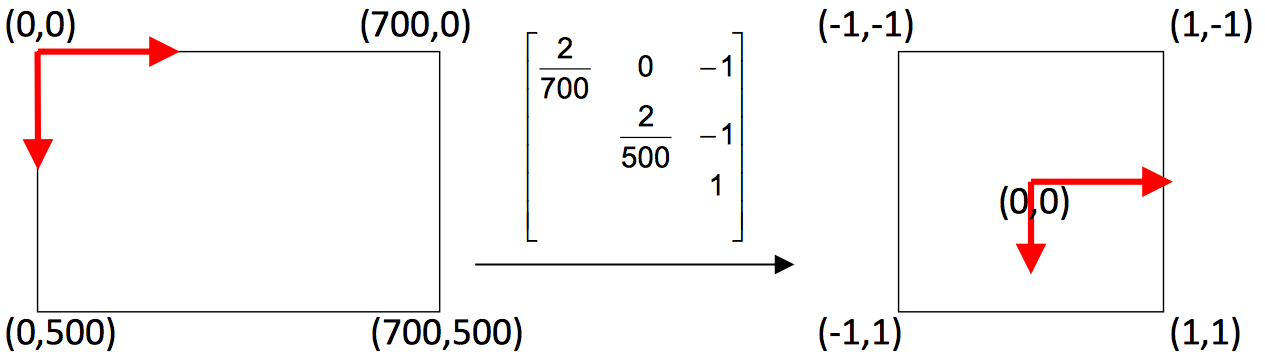
\includegraphics[scale=0.3]{pics/shift}
\caption{Shift for normalized algorithm. \label{fig:shift}}
\end{center}
\end{figure}
A more popular is to rescale the two point sets such that the centroid of each is 0 and the mean standard deviation $\sqrt{2}$. This can be done for every point as follows
\begin{equation}
\hat{p}^i=\frac{\sqrt{2}}{\sigma}\cdot (p^i-\mu),
\end{equation}
where
\begin{equation}
\mu=\frac{1}{N}\sum_{i=1}^n p^i
\end{equation}
is the centroid of the set and $\sigma=\frac{1}{N}\sum_{i=1}^n ||p^i-\mu||^2$ is the mean standard deviation. This transformation can be expressed in matrix form
\begin{equation}
\hat{p}^i=\begin{pmatrix}
\frac{\sqrt{2}}{\sigma}&0&-\frac{\sqrt{2}}{\sigma}\mu^x\\
0&\frac{\sqrt{2}}{\sigma}&-\frac{\sqrt{2}}{\sigma}\mu^y\\
0&0&1
\end{pmatrix}\cdot p^i.
\end{equation}
The algoritm at the end reads
\begin{enumerate}
\item Normalize point correspondences: $\hat{p}_1=B_1\cdot p_1$, $\hat{p}_2=B_2\cdot p_2$.
\item Estimate $\hat{F}$ using normalized coordinates $\hat{p}_1,\hat{p}_2$.
\item Compute $F$ from $\hat{F}:$
\begin{equation}
\begin{split}
\hat{p}_2^T\cdot \hat{F}\cdot \hat{p}_1&=0\\
 p_2^{T}\cdot B_2^T\cdot \hat{F}\ \cdot B_1\cdot p_1&=0\\
\Rightarrow F&=B_2^T\cdot \hat{F}\cdot B_1
\end{split}
\end{equation}
A valid fundamental matrix must have $\# $ rank =  $\# $ points and hence det(F)=0 
\end{enumerate}
\end{answer}
\item \textit{Quality metrics for Fundamental matrix estimation (directional error, epipolar line, and reprojection error).}
\begin{answer} We need to check the numerical results because there are orders of magnitude difference
between the columns  $\rightarrow$ least-squares yields poor results\\
\textbf{Directional Error}
Sum of the angular distances to the Epipolar plane: $err=\sum_i (\cos(\theta_i))^2$, where
\begin{equation}
cos(\theta)=\left(\frac{p_2^T\cdot E \cdot p_1}{||p_2^T||\cdot ||E\cdot p_1||} \right)
\end{equation}
\textbf{Epipolar Line Distance}
Sum of \textbf{Squared Epipolar-Line-to-point Distances}
\begin{equation}
err=\sum_{i=1}^Nd^2(p_1^i,l_1^i)+d^2(p_2^i,l_2^i).
\end{equation}
Cheaper than reprojection error: does not require point triangulation!
\begin{figure}[h!]
\begin{center}
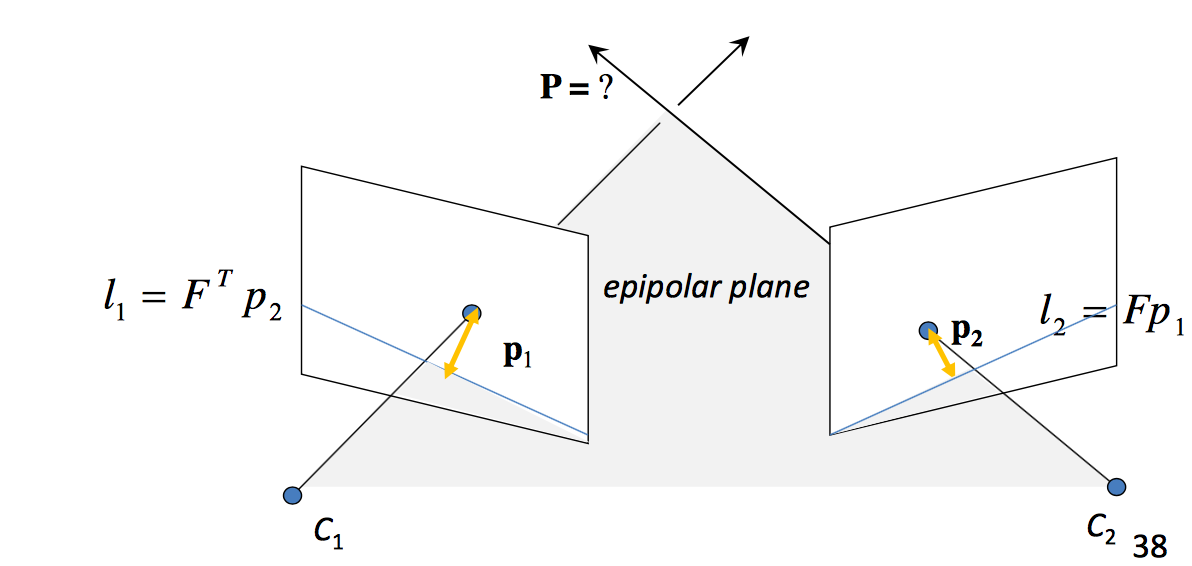
\includegraphics[scale=0.2]{pics/epi_line}
\caption{Epipolar Line Distance. \label{fig:epi_line}}
\end{center}
\end{figure}
\subsubsection*{Reprojection Error}
Sum of the \textbf{Squared Reprojection Errors}
\begin{equation}
err=\sum_{i=1}^N ||p_1^i-\pi_1(P^i)||^2+||p_2^i-\pi_2(P^i,R,T)||^2
\end{equation}
Computation is expensive because of point triangulation, but is the \textbf{most accurate}!
\begin{figure}[h!]
\begin{center}
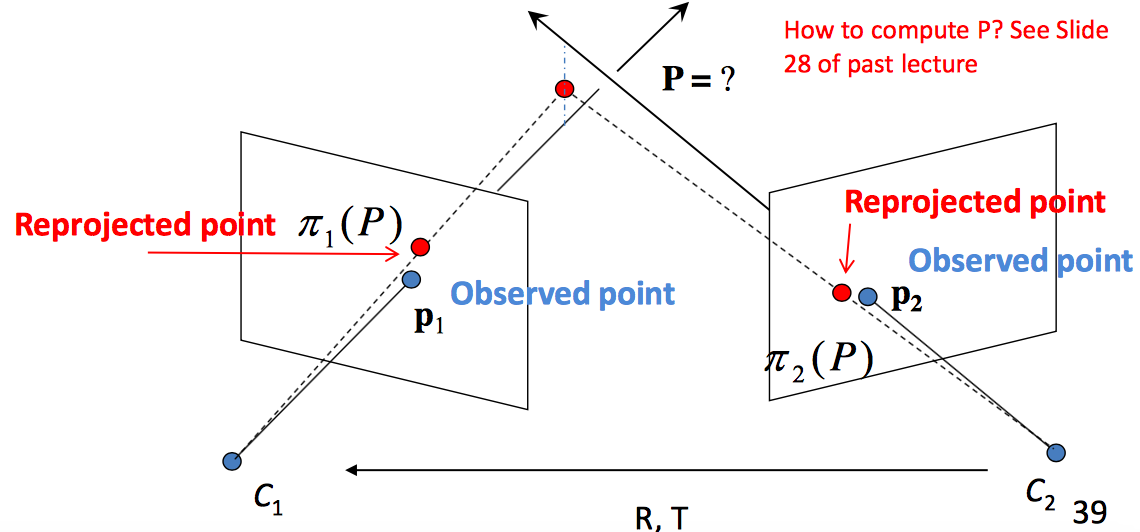
\includegraphics[scale=0.2]{pics/repro}
\caption{Reprojection Error. \label{fig:repro}}
\end{center}
\end{figure}
\end{answer}
\end{enumerate}

\subsection*{RANSAC}
\begin{enumerate}
\item \textit{Why do we need RANSAC?}
\begin{answer}
Matched points are usually contaminated by \textbf{outliers}. Causes for this are
\begin{itemize}
\item Change in view point and illumination
\item Image noise
\item Occlusions
\item Blur
\end{itemize}
The task of removing them is for \textbf{Robust Estimation}. 
\end{answer}
\item \textit{What is the theoretical maximum number of combinations to explore? }
\begin{answer}
Ransac is the standard method for \textbf{model fitting in the presence of outliers} (noise points or wrong data). It can be applied to all problems where the goal is to estimate parameters of a model from the data. An easy example is RANSAC for \textbf{line fitting:}
\begin{enumerate}
\item Select sample of 2 points at random.
\item Calculate model parameters that fit the data in the sample.
\item Calculate error function for each data point.
\item Select data that supports current hypothesis.
\item Repeat.
\item Select the set with the maximum number of inliers obtained within $k$ iterations.
\end{enumerate}
Theoretical \textbf{ maximum} number combinations to explore $N(N-1)/2$. Computationally unfeasibe if N is too large!
\end{answer}

 \item \textit{After how many iterations can RANSAC be stopped to guarantee a given success probability?}
\begin{answer}
Let $w$ be the number of inliers/$N$, $N$ be the total number of data points. We can think of $w$ as
\begin{equation}
w=P(\text{selecting an inlier-point out of the dataset}).
\end{equation}
We assume that the 2 points necessary to estimate a line are selected independently, i.e.
\begin{equation}
\begin{split}
w^2&=P(\text{both selected points are inliers})\\
1-w^2&=P(\text{at least one of these two points is outlier})\\
\end{split}
\end{equation}
Let $k$ indicate the number of RANSAC iterations so far, then
\begin{equation}
(1-w^2)^k=P(\text{RANSAC never selected two points both inliers})
\end{equation}
Let $p$ be the probability of success:
\begin{equation}
\begin{split}
1-p&=(1-w^2)^k\\
\Rightarrow k&=\frac{\text{log}(1-p)}{\text{log}(1-w^2)}.
\end{split}
\end{equation}

\end{answer}
\item \textit{What is the trend of RANSAC iterations $k$ vs the fraction of outliers $\varepsilon=1-w$ vs the minimum number of points to estimate the model? }
\begin{answer}
\
\begin{itemize}
\item As observed, $k$ is exponential in the number of points $s$ necessary to estimate the model. We can see that $k$ increases exponentially with the fraction of outliers $\varepsilon$.
\item The 8-point algorithm is extremely simple and was very successful; however it requires more than 1177 iterations.
\item The 5-point algorithm only requires 145 iterations, but can return up to 10 solutions of $E$.
\item The 2-point algorithm (e.g. line fitting) requires 16 iterations. Motion constraints need to be set to apply this algorithms for robots
\item The 1-point algorithm requires only 1 iteration and is \textbf{only} used to find the inliers. the motion is then estimated from them in 6DOF and only 1 DOF 
\end{itemize}
\end{answer}
\item \textit{How do we apply RANSAC to the 8-point algorithm vs DLT? }
\begin{answer}
DLT 6 points , don't need to since it's monocular and only one image. No outlier rejection for matching required, since there is no matching.\\
RANSAC 8 points. Needs outlier rejection, since stereo view $\rightarrow$ two images. The model with eight point algorithm is the matrix $E$.
\end{answer}
\item \textit{How can we reduce the number of RANSAC iterations
for the SFM problem (1- and 2-point RANSAC)?}
\begin{answer}
By choosing lower $p$ or another $w$, we can reduce the iterations. \\
\textbf{Planar Motion (1-,2-point RANSAC)}
Planar motion is described by three parameters $\vartheta,\varphi,\rho$
\begin{equation}
R=\begin{pmatrix}
\cos(\theta)&-\sin(\theta)&0\\
\sin(\theta)&\cos(\theta)&0\\
0&0&1
\end{pmatrix}, \qquad T=\begin{pmatrix}
\rho \cos(\varphi)\\
\rho \sin(\varphi)\\
0
\end{pmatrix}
\end{equation}
\begin{figure}[h!]
\begin{center}
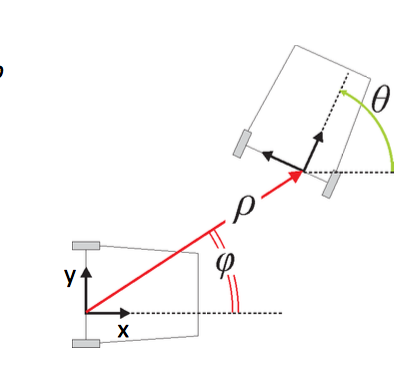
\includegraphics[scale=0.35]{pics/planar_motion}
\caption{Planar motion. \label{fig:planar_motion}}
\end{center}
\end{figure}
Let's compute the Epipolar Geometry
\begin{equation}
\begin{split}
E&=[T]_x\cdot R\\
&=\begin{pmatrix}
0&0&\rho \sin(\varphi)\\
0&0&-\rho \cos(\varphi)\\
-\rho \sin(\varphi)&\rho \cos(\varphi)&0
\end{pmatrix}\cdot \begin{pmatrix}
\cos(\theta)&-\sin(\theta)&0\\
\sin(\theta)&\cos(\theta)&0\\
0&0&1
\end{pmatrix}\\
&=\begin{pmatrix}
0&0&\rho \sin(\varphi)\\
0&0&-\rho \cos(\varphi)\\
-\rho \sin(\varphi-\theta)&\rho\cos(\varphi-\theta)&0
\end{pmatrix}.
\end{split}
\end{equation}
$E$ has 2 DoF ($\theta$, $\varphi$), because $\rho$ is the scale factor. Thus, 2 correspondences are sufficient to estimate them.\\
But: can we use \textbf{less} than 2 point correspondences? Yes, if we exploid wheeled vehicles with \textbf{non-holonomic} constraints. Wheeled vehicles like cars, follow locally-planar circular motion about the instantaneous Center of Rotation (ICR). Since $\varphi=\theta/2$, meaning that we have only 1 DoF. Only 1 point correspondence is needed. \textbf{This is the smallest parametrization possible and results in the most efficient algorithm for removing outliers (Scaramuzza)}. This updates the problem to be
\begin{equation}
R=\begin{pmatrix}
\cos(\theta)&-\sin(\theta)&0\\
\sin(\theta)&\cos(\theta)&0\\
0&0&1
\end{pmatrix}, \qquad T=\begin{pmatrix}
\rho \cos(\frac{\theta}{2})\\
\rho \sin(\frac{\theta}{2})\\
0
\end{pmatrix}
\end{equation}
and
\begin{equation}
\begin{split}
E&=[T]_x\cdot R\\
&=\begin{pmatrix}
0&0&\rho \sin(\frac{\theta}{2})\\
0&0&-\rho \cos(\frac{\theta}{2})\\
\rho \sin(\frac{\theta}{2})&-\rho\cos(\frac{\theta}{2})&0
\end{pmatrix}.
\end{split}
\end{equation}
With the Epipolar Geometry constraint leads to
\begin{equation}
\theta = -2 \tan^{-1}\left(\frac{v_2-v_1}{u_2+u_1} \right).
\end{equation}
Only one iteration: compute $\theta$ for every point correspondence.
Up to 1000 Hz, 1-point RANSAC in only used to find the inliers. Motion is then estimated from them in 6DOF.
\begin{figure}[h!]
\begin{center}
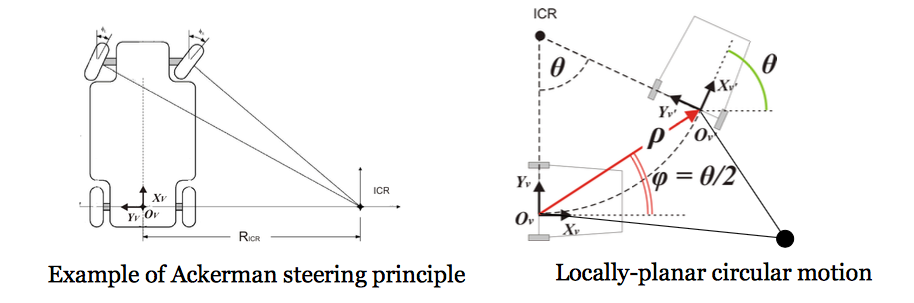
\includegraphics[scale=0.4]{pics/holonomic}
\caption{Non-holonomic. \label{fig:holonomic}}
\end{center}
\end{figure}
\end{answer}
\item \textit{In practice, can you fully rely on the formula that predicts the optimal number of iterations? (hint: especially when the inliers themselves are noisy, RANSAC exercise).}
\begin{answer}

\end{answer}
\end{enumerate} 

\subsection*{Bundle Adjustment}
\begin{enumerate}
\item \textit{Definition of Bundle Adjustment (mathematical expression and illustration). }
\begin{answer}
\textbf{Nonlinear, simultaneous refinement of structure and motion (i.e. $R,T,P^i$).} It is used after linear estimation of $R$ and $T$. This, computes $R,T,P^i$ by minimizing the Sum of Squared Reprojection Errors:
\begin{equation}
(R,T,P^i)=\text{argmin}_{R,T,P^i} \sum_{i=1}^N ||p_1^i-\pi_1(P^i,C_1)||^2+||p_2^i-\pi_2(P^i,C_2)||,
\end{equation}
where $C_1,C_2$ are the \textbf{pose} of the camera in the \textbf{world frame}. This can be minimized using \textit{Lavenberg-Marquardt} (more robust than Gauss-Newton to local minima). \textbf{It is better to initialize it close to the minimum.} Same for multiple views!
\begin{figure}[h!]
\begin{center}
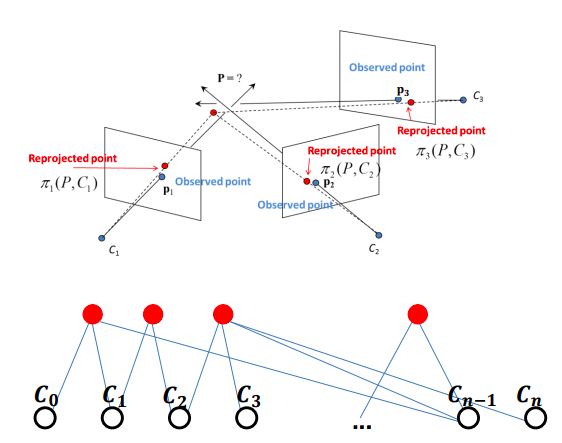
\includegraphics[scale=0.4]{pics/BAnview}
\caption{Bundle Adjustment n views. \label{fig:BA}}
\end{center}
\end{figure}
\end{answer}

\item \textit{Hierarchical SFM and sequential SFM for monocular VO. }
\begin{answer}
\textbf{Hierarchical SFM}
\begin{enumerate}
\item Extract and match features between nearby frames.
\item Identify clusters consisting of 3 nearby frames:
\item Compute SFM for the 3 frames:
\begin{itemize}
\item Compute SFM between 1 and 2 and build pointcloud.
\item Merge 3rd view running 3-point RANSAC between point cloud and 3rd view.
\end{itemize}
\item Merge clusters pairwise and refine (BA) both structure and motion. 
\end{enumerate}
Example is \textit{building Rome in one day}.\\
\textbf{Sequential SFM}\\
With $n$ views. Also called Visual Odometry (VO). 
\begin{enumerate}
\item \textbf{Bootstrapping}
\begin{itemize}
\item Initialize structure and motion from 2 views: e.g. 8-point algorithm + RANSAC.
\item Refine structure and motion (BA)
\item How far should the frames be? If too small baseline, large depth uncertainty. If too large baseline, small depth uncertainty.
Remember the picture with ellipses which describe the depth uncertainty. If baseline increases, the ellipses decrease in size.
\end{itemize}
\item \textbf{Localization}
\begin{itemize}
\item Compute camera pose from known 3D-to-2D feature correspondence. 
\begin{itemize}
\item Extract correspondences by solving for $R$ and $t$ ($K$ is known).
\begin{equation}
 \lambda \cdot \begin{pmatrix}
 u\\
 v\\
 1
 \end{pmatrix}=K\cdot [R|T]\cdot \begin{pmatrix}
 X_w\\
 Y_w\\
 Z_w\\
 1
 \end{pmatrix}
 \end{equation}
\end{itemize}
 \item What is the minimal number of required point correspondences
\begin{itemize}
\item 6 for linear solution (DLT algorithm).
\item 3 for a non linear solution (P3P algorithm).
\item 3 point RANSAC.
\end{itemize}
\end{itemize}
\item \textbf{Extend Structure}
\begin{itemize}
\item Extract and triangulate new features from keyframes
\end{itemize}
By denoting the relative motion between adjacent keyframes as
\begin{equation}
T_k=\begin{pmatrix}
R_{k,k-1}&t_{k,k_1}\\
0&1
\end{pmatrix},
\end{equation}
we can concatenate transformations to find the full trajectory of the camera as
\begin{equation}
C_k=T_{k,k-1}\cdot C_{k-1}
\end{equation}
\end{enumerate}
A non-linear refinement (BA) over the last $m$ poses (+visible structure) can be performed to get a more accurate estimate of the local trajectory. 
\end{answer}

\item \textit{ What are keyframes? Why do we need them and how can we select them? }
\begin{answer}
A data set may have a lot of images, but we don't need to run SFM algorithms on all images (computationally too expensive) to reconstruct a trajectory. A keyframe is an image for which the pose is estimated. Landmarks are triangulated using 2 keyframes as input. \\
When frames are taken at nearby positions compared to the scene distance, 3D points will exibit large uncertainty $\Rightarrow$ One way to avoid this consists of \textbf{skipping frames} until average uncertainty of the 3D points decreases below a certain threshold. The selected frames are called \textbf{keyframes}. In general
\begin{equation}
\frac{\text{keyframe distance}}{\text{average-depth}}>\text{threshold }(10-20\%).
\end{equation}
\end{answer}
\item \textit{Definition of loop closure detection (why do we need loops?). }
\begin{answer}
\
\begin{itemize}
\item Relocalization problem: during VO, tracking can be lost (due to occlusions, low tecture, quick motion, illumination change).
\item Solution is to re-localize camera pose and continue.
\item Loop closing problem: when go back where you already have been:
\begin{itemize}
\item Loop detection: to avoid map duplication (e.g. same crossing rotated)
\item Loop correction: to compensate the accumulated drift!
\end{itemize}
\item In both cases places recognition is needed (lecture 12)
\end{itemize}
\end{answer}
\item \textit{List the most popular open source VO and VSLAM algorithms. }
\begin{answer}
\
\begin{itemize}
\item PTAM: Parallel Tracking and Mapping for Small AR Workspaces
\item ORB-SLAM: Feature based, FAST corner + Oriented Rotated Brief descriptor includes loop closing, relocalization, final optimization, real time
\item LSD-SLAM: Direct (photometric error) + Semi-Dense formulation, includes loop closing, relocalization, final optimization, real time
\item DSO: Direct (photometric error) + Sparse formulation, real time, BA sliding window
\item SVO: Direct (minimizes photometric error), Feature-based (minimizes reprojection error), mapping, real time fast
\end{itemize}
\end{answer}
\item \textit{Differences between feature-based and direct methods.}
\begin{answer}
\textbf{Feature-based Methods}
\begin{enumerate}
\item Extract and match features (+RANSAC)
\item Minimize Reprojection Error:
\begin{equation}
T_{k,k-1}=\text{argmin}_T\sum_{i}||u_i'-\pi(p_i)||_\Sigma^2
\end{equation}
\textbf{Good:} Large frame-to-frame motions, accuracy and efficient optimization of SFM (BA).\\
\textbf{Bad:} Slow due to costly feature extraction and matching, matching outliers (RANSAC).
\end{enumerate}
\textbf{Direct Methods (all pixels)}
\begin{enumerate}
\item Minimize \textbf{photometric error}:
\begin{equation}
T_{k,k-1}=\text{argmin}_T\sum_{i}||I_k(u_i')-I_{k-1}(u_i)||_\sigma^2,
\end{equation}
where
\begin{equation}
u_i'=\pi(T\cdot (\pi^{-1}(u_i)\cdot d))
\end{equation}
\textbf{Good}: All information in the image can be exploited. Increasing camera frame-rate reduces computational cost per frame.\\
\textbf{Bad:} Limited frame to frame motion. Joint optimization of dense structures and motion too expensive.
\end{enumerate}
Feature based methods process the image to find corners to compare. This is an issue, as it doesn't work well in human environments, as many any straight or curved edges would be discarded, meaning that the information is less complete. Also, a picture which has most of its features concentrated in a small area is of less interest to the algorithm as a picture with many details all over, as the \textit{features} cannot overlap. Another issue with feature based methods is that storing the processed features can quickly become very costly. However, since this method eliminates all data that cannot be used (non features points), it is faster than direct methods. It is possible to reconstruct dense maps from feature based methods by estimating the camera positions to find what was at the given location.\\ \\
Direct Methods however, compare the entire images to each other to reference them to each other, finding which parts go together. It can create semi dense 3D maps in real time on a smartphone using semi dense filtering algorithms. This means it provides more information about he environment, making it more interesting to use in robotics or Augmented Reality, as well as giving a more meaningful representation to the human eye. Some disadvantages of Direct methods are that they cannot handle outliers very well, as they will always try to process them an implement them into the final map, and that they are slower than feature based variants. 
\begin{figure}[h!]
\begin{center}
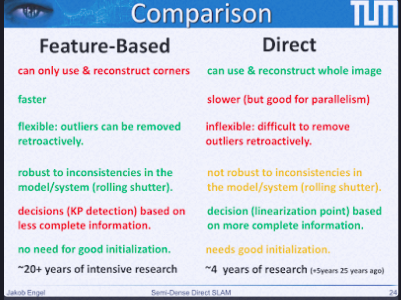
\includegraphics[scale=0.65]{pics/direct}
\caption{Comparison direct vs feature based. \label{fig:direct}}
\end{center}
\end{figure}
\end{answer}


\end{enumerate}

\newpage
\section*{Lecture 10 Multi view stereo}
\begin{enumerate}
\item \textit{Working principle (aggregated photometric error). }
\begin{answer}
For the 3D reconstruction from multiple views, we assume that camera are calibrated
\begin{itemize}
\item \textbf{intrinsically} ($K$ is known for each camera), and
\item \textbf{extrinsically} ($T$ and $R$ between cameras are known, for instance, from SFM).
\end{itemize}
For the multi-view stereo, we have as:\\
\textbf{Input}: calibrated images from several viewpoints. \\
From a \textit{dense} region of pixels (hence not only from corners) estimate the structure. The workflow is:
\begin{enumerate}
\item \textbf{Local methods}: estimate depth for every pixel independently. (Not all the pixels can be matched reliably, due to viewpoint changes, occlusions.)\\
We take advantage of \textit{many} small baseline views, where \textit{high quality} matching is possible. 
\item \textbf{Global methods}: refine the depth surface as a whole by enforcing smoothness constraint.\\
We use the \textbf{photometric error} (SSD): the aggregated photometric error plot is derived for every combination of the reference image and any further image. \textbf{IDEA}: optimal depth minizes the photometric error in all images as a function of the depth in the first image.\\
The SSD between corresponding patches of intensity values (min patch size: $1\times 1$ pixels) = photometric error $\rightarrow$ dense correspondences $\rightarrow$ dense reconstruction
\end{enumerate}
\textbf{Output}: 3D object dense reconstruction. \\
Recall: The two camera centers and the image point $p$ determine the epipolar plane, which intersects each camera image plane in the epipolar lines. Since we use the epipolar constraint, corresponding points only need to be searched along epipolar lines.
\end{answer}
\item \textit{What are the differences in the behavior of the aggregated photometric error for corners, flat regions, and edges?}
\begin{answer}
Plot: x-axis inverse depth d, y-axis aggregated photometric error C(a,d), a= image point
\begin{itemize}
\item The aggregated photometric error for \textit{flat regions} and \textit{edges} parallel to the epipolar line show \textbf{flat valleys} (noise!).
\item For distinctive features like corner, the aggregated photometric error has one clear minimum.
\item Repetitive texture shows multiple minima.
\end{itemize}
\end{answer}

\item \textit{What is the Disparity Space Image (DSI) and how is it built in practice? }
\begin{answer}
For a given image point $(u,v)$ and for discrete depth hypotheses $d$, the aggregate photometric error $C(u,v,d)$ with respect to the reference image $I_r$ can be stored in a volumetric 3D grid called the \textit{Disparity Space Image (DSI)}, where each voxel (group of $u,v,d$) has value
\begin{equation}
C(u,v,d)=\sum_{k}\underbrace{\rho \left( \tilde{I}_k (u',v',d)-I_r(u,v)\right)}_{photometric error (SSD)},
\end{equation}
where $\tilde{I}_k (u',v',d)$ is the patch of intensity values in the $k$-th image centered on the pixel $(u',v')$ corresponding to the patch $I_r(u,v)$ in the reference image $I_r$ an depth hypothesis $d$. 
\end{answer}

\item \textit{ How do we extract the depth from the DSI?}
\begin{answer}
The depth is the solution to a function $d(u,v)$ in the DSI that satisfies:
\begin{equation}
\begin{split}
&\text{Minimum aggregated photometric error (i.e. } argmin_d C)\\
& \text{AND}\\
& \text{Piecewise smooth (global methods)}
\end{split}
\end{equation}
Interpolating while not overfitting!\\

\end{answer}
\item \textit{How do we enforce smoothness (regularization) and how do we incorporate depth discontinuities (mathematical expressions)? }
\begin{answer}
\textbf{Global Methods:} We smooth the image in terms of energy minimization. The objective is to find a surface $d(u,v)$ that minimizes a global energy
\begin{equation}
E(d)=\underbrace{E_d(d)}_{\text{data term}}+\underbrace{\lambda \cdot E_s(d)}_{\text{regularization term}},
\end{equation}
where 
\begin{equation}
E_d(d)=\sum_{(u,v)} C(u,v,d(u,v))
\end{equation}
and
\begin{equation}
E_s(d)=\sum_{(u,v)}\rho_d(d(u,v)-d(u+1,v))+\rho_d(d(u,v)-d(u,v+1)).
\end{equation}
$\rho_d$ is a norm (e.g. the $L_{1,2}$ or Huber norm). 
\end{answer}
\begin{itemize}
\item \textbf{The regularization term} $E_s(d)$
\begin{itemize}
\item \textbf{Smooths} non smooth surfaces (result of noisy measurements) as well as discontinuities.
\item Fills the holes.
\end{itemize}
\item Popular assumption: discontinuities in intensity \textbf{coincide} with discontinuities in depth.
\item Control \textbf{smoothness penalties} according to image gradient (discrete)
\begin{equation}
\rho_d(d(u,v)-d(u+1,v))\cdot \rho_I(||I(u,v)-I(u+1,v)||)
\end{equation}
\item $\rho_I$ is some monotically \textit{decreasing} function of intensity differences: \textbf{lower} smoothness cost for \textbf{high intensity gradients} (if there are high intensity gradients, you don't want to smooth them as they are a crucial information in your image.
\end{itemize}

\item \textit{What happens if we increase lambda (the regularization term)? What if lambda is 0? And if lambda is too big?}
\begin{answer}
$\lambda$ controls the tradeoff data (regularization) 
\begin{itemize}
\item Higher $\lambda$ =  higher \textbf{smoothing}!
\item $\lambda = 0 \rightarrow$  no smoothing
\item $\lambda$ too big $\rightarrow$ oversmoothing. can't recognize different depths anymore
\end{itemize}
 
\end{answer}

\item \textit{What is the optimal baseline for multi-view stereo?}
\begin{answer}
\
\begin{itemize}
\item Too small: large depth error.
\item Too large: difficult search problem.
\end{itemize}
\textbf{Solution}: 
\begin{itemize}
\item Obtain depth map from small baselines
\item When baseline becomes too large create new reference frame (keyframe) and start new depth computation
\end{itemize}
A possible approach is \textbf{depth map fusion} (different depth maps with different perspectives gives a complete image).
\end{answer}
\item \textit{What are the advantages of GPUs?}
\begin{answer}
General Purpose Computing on Graphics Processing Unit. It can perform more demanding calculations than CPU because
\begin{itemize}
\item GPUs run thousand of lightweight threads \textbf{in parallel}
\begin{itemize}
\item more transistors for data processing.
\item Typically on consumer hardware: 1024 threads per multiprocessor, 30 multiprocessors: 30000 threads. CPU with 4 cores which supports 32 threads. 
\end{itemize}
\item well suited for \textbf{data-parallelism} 
\begin{itemize}
\item the same instructions executed on multiple data in parallel
\item high \textbf{arithmetic intensity}: arithmetic operations/ memory operations
\end{itemize}
\end{itemize}
Those characteristics lead to
\begin{itemize}
\item Fast pixel processing (ray tracing, draw textures, shaded triangles,..)
\item Fast matrix/vector operations (transform vertices)
\item Programmable (shading, bump mapping)
\item Floating-point support (accurate computations)
\item Deep learning.
\end{itemize}
\end{answer}
\end{enumerate}
\newpage
\section*{Lecture 11 Tracking}
\begin{enumerate}
\item \textit{Illustrate tracking with block matching.}
\begin{answer}
Block matching is an approach for point tracking. given two images, estimate the motion of a pixel point from image\_1 to image\_2
\begin{itemize}
\item Search for the corresponding patch in a \textit{neighborhood} around the point.
\item Use SSD, SAD, NCC to search for corresponding patches in a local neighborhood of the point. The search region usially is a $D\times D$ squared patches. We have to perform $D\times D$ comparisons, computationally demanding.
\end{itemize}
\begin{figure}[h!]
\begin{center}
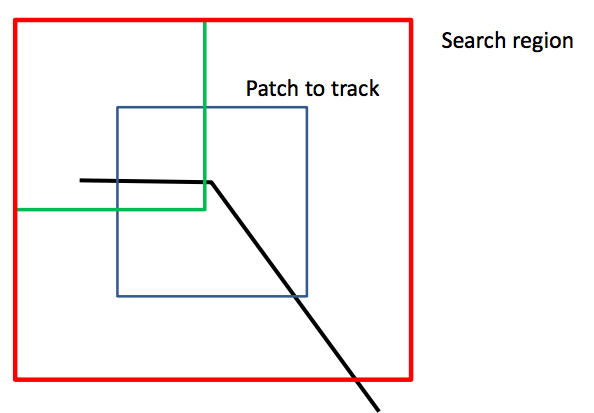
\includegraphics[scale=0.35]{pics/block_matching}
\caption{Block matching. \label{fig:blockmatch}}
\end{center}
\end{figure}
\end{answer}
\item \textit{Differential Methods}
\begin{enumerate}
\item \textit{Describe the underlying assumptions, derive the
mathematical expression, and meaning of the M matrix.}
\begin{answer}
\
\begin{itemize}
\item Look at the local brightness changes at the \textbf{same} location. \textbf{NO patch shift} is performed. (centered in the same point!)
\end{itemize}
\textbf{Spatial Coherency} We assume that all the pixels in the patch undergo the same motion (same $u$ and $v$). Also, assume that the time interval between the two images $I_0$ and $I_1$ is small. We want to find the motion vector $(u,v)$ that minimizes the Sum of Squared Differences (SSD). As we did for Harris, we look at the first order Taylor approximation of the sum:
\begin{equation}
\begin{split}
SSD&=\sum(I_0(x,y)-I_1(x+u,y+v))^2 \\
&\approx \sum(I_0(x,y)-I_1(x,y)-I_x\cdot u -I_y \cdot v)^2\\
&=\sum(\Delta I-I_x\cdot u - I_y \cdot v)^2\\
&= E, 
\end{split}
\end{equation}
which is a simple quadratic function in two variables $(u,v)$. To minimize the $E$, we differentiate with respect to $(u,v)$ and equate to 0.
\begin{equation}
\begin{split}
\frac{\partial E}{\partial u}&=0 \Rightarrow -2I_x \sum(\Delta I-I_x\cdot u - I_y \cdot v)=0\\
\frac{\partial E}{\partial v}&=0 \Rightarrow -2I_y \sum(\Delta I-I_x\cdot u - I_y \cdot v)=0
\end{split}
\end{equation}
Linear system of two equations in two unknowns. We can write this in matrix form
\begin{equation}
\begin{split}
\begin{pmatrix}
\sum I_xI_x & \sum I_x I_y\\
\sum I_xI_y & \sum I_y I_y
\end{pmatrix} \cdot \begin{pmatrix}
u\\ v 
 \end{pmatrix}&= \begin{pmatrix}
 \sum I_x \cdot \Delta I\\
  \sum I_y \cdot \Delta I\\
 \end{pmatrix}\\
 \begin{pmatrix}
u\\ v 
 \end{pmatrix}&=\underbrace{\begin{pmatrix}
\sum I_xI_x & \sum I_x I_y\\
\sum I_xI_y & \sum I_y I_y
\end{pmatrix}}_{M} ^{-1}\cdot \begin{pmatrix}
 \sum I_x \cdot \Delta I\\
  \sum I_y \cdot \Delta I\\
 \end{pmatrix}
 \end{split}
\end{equation}
These are not matrix products, but pixel-wise products!
\end{answer}
\item \textit{When Is this matrix invertible and when not? }
\begin{answer}
For $M$ to be invertible, its determinant should be non 0. From the decomposition 
\begin{equation}
M=R^{-1}\cdot \begin{pmatrix}
 \lambda_1 &0\\
 0&\lambda_2
 \end{pmatrix}\cdot R,
\end{equation}
we know that $\det(M)$ is non zero when its eigenvalues are large (i.e. not a flat region and not an edge). In practice, it should be a corner or in general contain \textbf{texture}.
\end{answer}
\item \textit{What is the aperture problem and how can we overcome it? }
\begin{answer}
If we look at local brightness changes through a small aperture, we cannot always determine the motion direction, because \textbf{infinite} motion directions (solutions) may exist (along a edge). The solution is to \textbf{increase} the aperture size.
\end{answer}
\item \textit{What is optical flow?}
\begin{answer}
Optical flow is an application of \textbf{differential method} and is the pattern of apparent motion of objects in a visual scene, caused by the relative motion between the observer (eye or camera) and the scene. It tracks the motion of every pixel between two consecutive frames. For each pixel, we compute
\begin{itemize}
\item The vector direction and,
\item The vector length (amount of movement).
\end{itemize}
An issue could be the choice of the right patch size. It can also be applied to corner tracking.
\end{answer}
\end{enumerate}
\item \textit{Pros and Cons of block-based vs differential methods for tracking}
\begin{answer}
\textbf{Block-based Methods}: search for the corresponding patch in a neighborhood of the point to be tracked. The search region is usually a square of $n\times n$ pixels. 
\begin{itemize}
\item $+$: \textbf{robust to large motions}
\item $-$: Can be computationally expensive ($n\times n$ comparisons for a single point track)
\end{itemize}
\textbf{Differential Methods}: 
\begin{itemize}
\item $+$: Much more efficient than block-based methods. Thus, can be used to track the motion of every pixel in the image. It avoids searching in the neighborhood of the point by analyzing the \textbf{local intensity changes} of an image patch at a specific location (no search is performed).
\item $-$: Works only for \textbf{small} motions (high frame rate). For larger motion, multiscale implementations are used, but are then expensive.
\end{itemize}
\end{answer}
\item Lucas-Kanade algorithm 
\begin{enumerate}
\item \textit{Working principle of KLT and derivation of the underlying mathematical expression (only first two slides titled “derivation of the Lucas-Kanade algorithm”, slide pp. 55-56)}
\begin{answer}
\textbf{Template Warping} Given the template image $T(x)$, take all the pixels from the template image and warp them using the function $W(x,p)$ parameterized in terms of parameters $p$. The goal of template-based tracking is to find the set of warp parameters $p$ such that
\begin{equation}
I(W(x,p))=T(x).
\end{equation}
Assumptions are:
\begin{itemize}
\item No errors in the template image boundaries: only the appearance of the object to be tracket appears in the template image.
\item No occlusion: the entire template is visible in input image.
\item Brightness consistency assumption: the intensity of the object appearance is always the same across different views. 
\end{itemize}
The \textbf{algorithm}:
\begin{enumerate}
\item Warp $I(x)$ with $W(x,p)$.
\item Compute the error.
\item Compute \textbf{warped} gradients, $\nabla I$ evaluated at $W(x,p)$.
\item Evaluate the Jacobian of the warping $\frac{\partial W}{\partial p}$.
\item Compute the inverse Hessian $H^{-1}$.
\item Multiply steepest descend with error.
\item Comptue $\Delta p$.
\item Update parameters $p \leftarrow p+\Delta p$.
\item Repeat until $\Delta p < \varepsilon$.
\end{enumerate}
The algorithm follows a predict-correct cycle. A prediction $I(W(x,p))$ of the warped image is computed from an initial estimate.\\
It uses the Gauss-Newton method for minimization, i.e.
\begin{itemize}
\item Applies a first order approximation of the warp,
\item Attempts to minimize the SSD iteratively.
\end{itemize}
This is solved by determining $p$ that minimizes the Sum of Squared Differences
\begin{equation}
E=SSD=\sum_{x\in T}\left[ I(W(x,p))-T(x)\right]^2.
\end{equation}
 Then, we want to find the increment $\Delta p$ that minimizes
\begin{equation}
\sum_{x\in T}\left[ I(W(x,p+\Delta p))-T(x)\right]^2.
\end{equation}
The first order Taylor approximation of the term in brackets reads
\begin{equation}
I(W(x,p+\Delta p))\approx I(W(x,p))+ \underbrace{\nabla I}_{\text{image gradient}} \underbrace{\frac{\partial W}{\partial p}}_{\text{Jabobianof the warp}}\Delta p.
\end{equation}
The image gradient $\nabla l=[I_x,I_y]$ is evaluated at W(x,p). By replacing that in the equation we get
\begin{equation}
E=\sum_{x\in T}\left[ I(W(x,p))+ \nabla I \frac{\partial W}{\partial p}\Delta p-T(x)\right]^2.
\end{equation}
In order to minimize it, we differentiate and equate to 0, i.e.
\begin{equation}
\frac{\partial E}{\partial \Delta p}=0.
\end{equation}
\end{answer}
\item \textit{What is the Hessian matrix and for which warping function does it coincide to that used for point tracking?}
\begin{answer}
\begin{equation}
\Delta p=H^{-1}\sum_{x\in T}\left( \nabla I \frac{\delta W}{\delta p}\right)^T(T(x)-I(W(x,p))),
\end{equation}
where
\begin{equation}
\ H=\sum_{x\in T}\left( \nabla I \frac{\partial W}{\partial p}\right)^T \left( \nabla I \frac{\partial W}{\partial p}\right)
\end{equation}
is the second moment matrix of the warped image (Hessian).\\
Translation ?
\begin{equation}
\nabla W_p = \begin{bmatrix}
1 & 0 \\
0 & 1
\end{bmatrix} \Rightarrow
\nabla I \nabla W_p = \begin{bmatrix}
I_x & 0\\
0 &I_y
\end{bmatrix} \Rightarrow
H = \begin{bmatrix}
I_x I_x & 0 \\
0 & I_y I_y
\end{bmatrix}
\end{equation}
\begin{figure}[h!]
\begin{center}
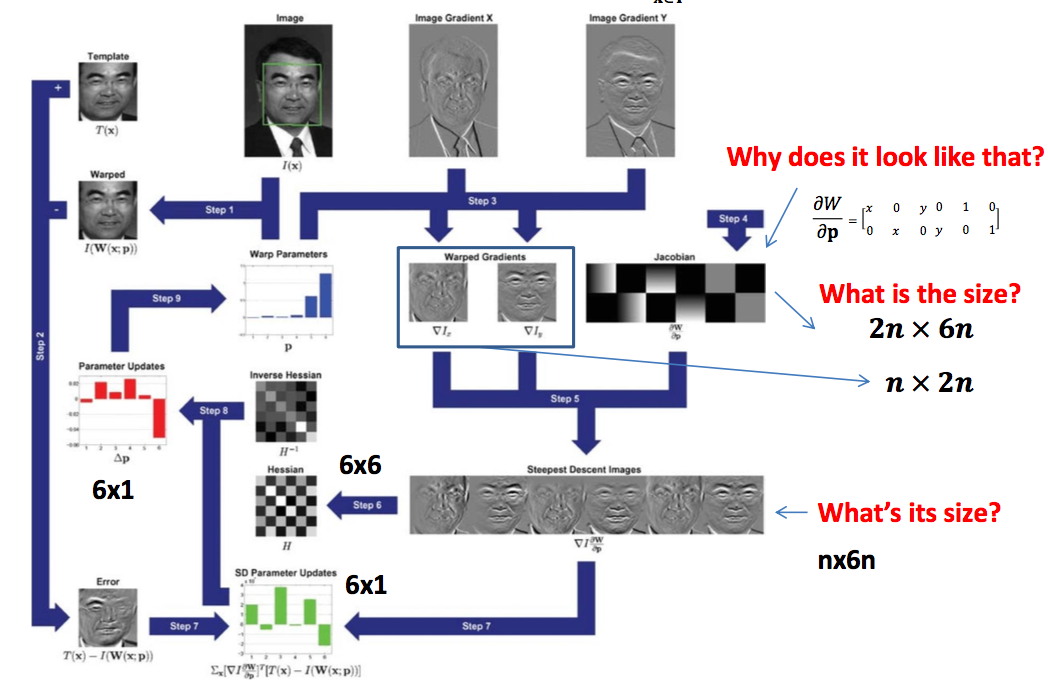
\includegraphics[scale=0.3]{pics/KLT}
\caption{KLT algorithm \label{fig:klt}}
\end{center}
\end{figure}
\end{answer}
\item \textit{Lucas-Kanade failure cases and how to overcome them}
\begin{answer}
\begin{itemize}
\item If the initial estimate is too far, the linear approximation does not longer hold. Or aliasing because many pixel have the same intensity.  Solution are \textbf{pyramidal implementations} / coarse-to-fine implementation
\item if Illumination changes, object deformations and Occlusions are in the initial image, the tracking will drift.  A solution can be to update the template with newest image.
\item In order to deal with wrong prediction, it can be implemented in a Particle-Filter fashion.
\end{itemize}
\end{answer}
\item \textit{How do we get the initial guess? }
\begin{answer}
We set the initial guess to zero $p = 0$ , because there is not initial guess available at the deepest pyramidal level.
\end{answer}
\item \textit{Illustration of coarse-to-fine Lucas-Kanade implementation. }
\begin{answer}
Due to the small motion assumption, regular optical flow methods work bad if the object we are tracking moves a long distance. Building image pyramids for each image and doing optical flow on each layer of the pyramid (to get rid of small motion constraints).For building the pyramid, first reduce the image resolution using Gaussian blur and then scale the image down.
\begin{figure}[h!]
\begin{center}
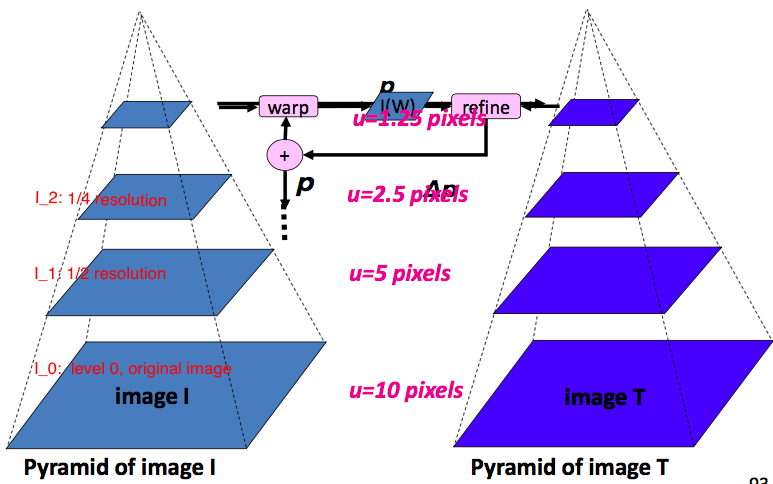
\includegraphics[scale=0.3]{pics/pyramid}
\caption{Pyramidal implementation. \label{fig:pyramid}}
\end{center}
\end{figure}
\end{answer}
\item \textit{llustrate alternative tracking using point features.}
\begin{answer}
\
\begin{enumerate}
\item Keypoint detection and matching. Invariant to scale, rotation or perspective.
\item Geometric verification (RANSAC)
\end{enumerate}
Issues here are:
\begin{itemize}
\item How to segment the object to track from background?
\item How to initialize the warping?
\item How to handle occlusions?
\item How to handle illumination changes andn on modeled effects?
\end{itemize}
\end{answer}
\end{enumerate}
\item \textit{List one or more possible ways of discarding wrong feature tracks in practice.}
\begin{answer}
???
\end{answer}

\end{enumerate}


\begin{center}
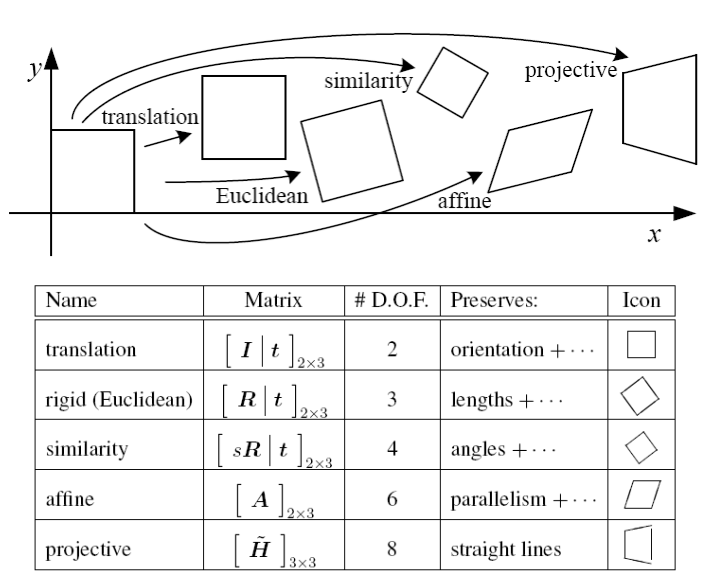
\includegraphics[scale=0.4]{pics/2Dtransfo}
\end{center}


\begin{itemize}
\item Warping function $W(x,p)$
\item \textbf{p} set of parameters $p = (a_1,a_2,...a_n)$
\item \textbf{Translation}: 2 DOF
\begin{equation}
W(x,p)=\begin{pmatrix}
x+a_1\\
y+a_2
\end{pmatrix}=\begin{pmatrix}
1&0&a_1\\
0&1&a_2
\end{pmatrix}\cdot \begin{pmatrix}
x\\
y\\
1 
\end{pmatrix}.
\end{equation}
\item \textbf{Euclidean}: 3 DOF
\begin{equation}
W(x,p)=\begin{pmatrix}
x\cos(\alpha)-y\sin(\alpha)+a_1\\
x\sin(\alpha)+y\cos(\alpha)+a_2
\end{pmatrix}=\begin{pmatrix}
\cos(\alpha)&\sin(\alpha)&a_1\\
\sin(\alpha)&\cos(\alpha)&a_2
\end{pmatrix}\cdot \begin{pmatrix}
 x\\
 y\\
 1
\end{pmatrix}.
\end{equation}
\item \textbf{Affine}: 6 DOF
\begin{equation}
W(x,p)=\begin{pmatrix}
a_1x+a_3y+a_5\\
a_2x+a_4y+a_6
\end{pmatrix}=\begin{pmatrix}
a_1&a_3&a_5\\
a_2&a_4&a_6
\end{pmatrix}\cdot \begin{pmatrix}
 x\\
 y\\
 1
 \end{pmatrix}.
\end{equation}
\item \textbf{Projective (homography)}: 8 DOF
\begin{equation}
x'=\frac{a_1x+a_2y+a_3}{a_7x+a_8y+1} , \quad y'=\frac{a_4x+a_5y+a_6}{a_7x+a_8y+1}.
\end{equation}
\begin{equation}
W(\tilde{x},p) = \begin{bmatrix}
a_1 &a_2& a_3\\
a_4& a_5 &a_6 \\
a_7 &a_8& 1
\end{bmatrix}
\begin{bmatrix}
x\\
y\\ 
1
\end{bmatrix}
\end{equation}
\end{itemize}
Recalling that the Jacobian of a function 
\begin{equation}
F(x_1,x_2,\hdots,x_n)=\begin{pmatrix}
f_1(x_1,x_2,\hdots,x_n)\\
\vdots \\
f_m(x_1,x_2,\hdots x_n)
\end{pmatrix}
\end{equation}
is
\begin{equation}
J(F)=\nabla F= \begin{pmatrix}
 \frac{\partial f_1}{\partial x_1}&\hdots & \frac{\partial f_1}{\partial x_n}\\
 &\vdots&\\
  \frac{\partial f_n}{\partial x_1}&\hdots & \frac{\partial f_n}{\partial x_n}\\
 \end{pmatrix}
\end{equation}
Displacement-model with Jacobians $\nabla W_p$
\newpage
\section*{Lecture 12 Place Recognition}
\subsection*{Bag of Words}
\begin{enumerate}
\item \textit{Inverted file index}
\begin{answer}
For text documents, an index is important. We want to find every image in which a feature occurs. How many SIFT or BRISK features exist ?
\begin{itemize}
\item SIFT: infinite.
\item BRISK-128: $2^{128}=2.4\cdot 10^{38}$.
\end{itemize}
For this reason, we need to create visual words, then put them into a vocabulary. Basically, we collect images and we extract features. A visual word is the centroid of a cluster. We then cluster the descriptors with the different words.\\
An \textbf{inverted file index} lists all visual words in the vocabulary (extracted at training time). Each word points to a list of images from the all image Data Base, in which which that word appears. The DB grows as the robot navigates and collects new images.\\
 \textbf{Voting Array}: has as many cells as the images in the DB. Each word in the query image votes for an image.
\end{answer}
\item \textit{What is a visual word?}
\begin{answer}
 A visual word is the centroid of a cluster and is a part of a \textbf{visual vocabulary}. \\
 Image collection $\rightarrow$ extract features $\rightarrow$ order the features based on their descriptors in the descriptor space $\rightarrow$ cluster the descriptors 
\end{answer}
\item \textit{ Why do we need hierarchical clustering? }
\begin{answer}
We need hierarchical clustering to build the \textbf{inverted file index} and enable the recognition.
\end{answer}
\item \textit{How does K-means clustering work?}
\begin{answer}
This is an algorithm to partition $n$ observations into $k$ clusters in which each observation $x$ belongs to the cluster $S_i$ with centroid $m_i$. It minimizes the sum of squared Euclidean distances between points $x$ and their nearest cluster centers $m_i$
\begin{equation}
D(X,M)=\sum_{i=1}^k\sum_{x \in S_i}(x-m_i)^2.
\end{equation}
The algorithm reads
\begin{enumerate}
\item Randomly initialize $k$ cluster centers
\item Iterate until convergence:
\begin{itemize}
\item Assign each data point $x_i$ to the nearest center $m_i$.
\item Recompute each cluster center as the mean of all points assigned to it.
\end{itemize}
\end{enumerate}
\end{answer}
\item \textit{ Explain and illustrate image retrieval with Bag of Words. }
\begin{answer}
Bag of Words can be applied to image classification, by treating image features as words. In document classification, a bag of words is a sparse vector of occurrence counts of words; that is, a sparse histogram over the vocabulary. In computer vision, a bag of visual words is a vector of occurrence counts of a vocabulary of local image features. \\
This algorithm simply computes the distribu-tion (histogram) of visual words found in the query image and compares this distribution to those found in the training images (vocabulary). 
\begin{figure}[h!]
\begin{center}
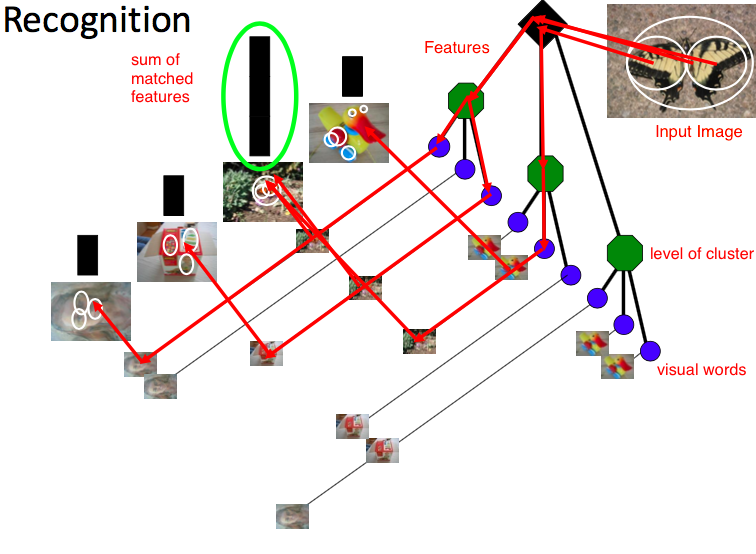
\includegraphics[scale=0.35]{pics/bowretrieval}
\caption{Bag-of-Words Retrieval. \label{fig:Bow}}
\end{center}
\end{figure}
\end{answer}
\item \textit{Discussion on place recognition: what are the open challenges and what solutions have been proposed?}
\begin{answer}
Visual Vocabulary discards the spatial relationships between features: two images with the same features shuffled around will return a 100\% match when using only appearance information. This can be overcome with \textbf{geometric verification}: test the $h$ most similar images to the query image for geometric consistency (5,8 point RANSAC) and retain the image with the smallest reprojection error and largest number of inliers. More words is better!
\end{answer}
\end{enumerate}
\newpage
\section*{Lecture 13 Visual Inertial Fusion}
Inertial Measurement Unit: angular velocity, linear acceleration\\

\begin{enumerate}
\item
\begin{enumerate}
\item \textit{Why an IMU for VO?}
\begin{answer}
\
\begin{itemize}
\item Monocular vision is scale ambiguous.
\item Pure vision is not robust enough (Tesla accident):
\begin{itemize}
\item Low texture.
\item High dynamic range.
\item High speed motion.
\end{itemize}
\end{itemize}
\textbf{Why not just IMU?}\\
Pure IMU integration will lead to large drift (especially cheap IMUs). Integration of angular velocity to get orientation: error \textbf{proportional to $t$}. Double integration to get position: if there is a bias in acceleration, the error of position is \textbf{proportional to $t^2$.} The actually position error also depends on the error of orientation.
\end{answer}
\item \textit{How does a MEMS IMU work? }
\begin{answer}
\
\begin{itemize}
\item Mechanical: spring/damper system.
\item Optical: Phase shift projected laser beams is proportional to angular velocity.
\item MEMS (accelerometer): a spring-like structure connects the device to a seismic mass vibrating in a capacitive divider. A capacitive divider converts the displacement of the seismic mass into an electric signal. Damping is created by the gas sealed in the device.
\item MEMS (gyroscopes): measure the Coriolis forces acting on MEMS vibrating structures. Their working principle is similar to the haltere of a fly.
\end{itemize}
\end{answer}
\item \textit{What’s the drift of an industrial IMU?}
\begin{answer}
Accelerometer Bias Error: 3 mg\\
Drift: 1s = 15 mm , 10s = 1.5m, 60s = 53 m 
\begin{itemize}
\item Integration of angular velocity to get orientation: error proportional to t Double integration of acceleration to get position: if there is a bias in
\item acceleration, the error of position is \textbf{proportional} to $t^2$
\item Worse, the actually position error also depends on the error of orientation.
\end{itemize}
\end{answer}
\end{enumerate}

\item \textit{What is the IMU measurement model (formula)? }
\begin{answer}
\begin{equation}
\begin{split}
\tilde{\omega}_{WB}^B(t)&=\omega_{WB}^B(t)+b^g(t)+n^g(t)\\
\tilde{a}_{WB}^B(t)&=R_{BW}(t)\cdot \left(a_{WB}^W(t)-g^W \right) + b^a(t)+n^a(t)
\end{split}
\end{equation}
where $g$ stands for Gyroscope and $a$ for accelerometer. The noise is additive Gaussian white noise. The bias has own dynamics
\begin{equation}
\dot{b}(t)=\sigma_b\cdot w(t),
\end{equation}
i.e. the derivative of the bias is white Gaussian noise (random walk). In discrete time, one writes
\begin{equation}
b[k]=b[k-1]+\sigma_{bd}\cdot w[k], \quad w[k]\sim \mathcal{N}(0,1), \quad \sigma_{bd}=\sigma_b\cdot \sqrt{t}
\end{equation}
\end{answer}
\item \textit{ What causes the bias in an IMU?}
\begin{answer}
Bias can be estimated.
\begin{itemize}
\item Can change due to temperature change, mechanical pressure,..
\item Can change everytime the IMU is started.
\end{itemize}

\end{answer}
\item \textit{How do we model the bias? }
\begin{answer}
Integration leads to
\begin{equation}
p_{Wt_2}=P_{Wt_1}+(t_2-t_1)v_{Wt_1}+\int \int_{t_1}^{t_2}R_{Wt}(t)\left( \tilde{a}(t)-b^a(t)+g^w \right)\text{d}t^2,
\end{equation}
which depends on initial position and velocity. The rotation $R(t)$ can be computed with a gyroscope.
\end{answer}
\item \textit{How do we integrate the acceleration to get the position (formula)? }
\begin{answer}
???
\end{answer}
\item \textit{Definition of Loosely coupled vs tightly coupled visual inertial fusion}
\begin{answer}
\textbf{Loosely Coupled Approach}: 
Treats VO and IMU as two separate (not coupled black boxes). Each block estimates \textbf{pose and velocity} from visual and inertial data (pose and velocity up to a scale and inertial data in absolute scale).
\begin{figure}[h]
\begin{center}
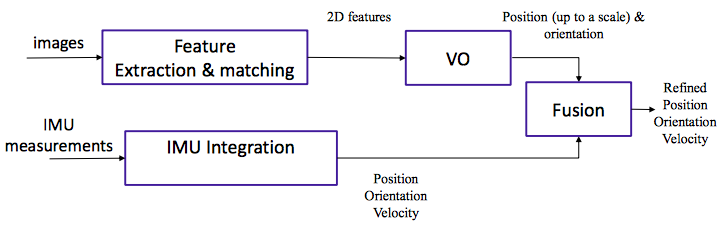
\includegraphics[scale=0.6]{pics/loos}
\caption{Loosely Coupled Approach.}
\end{center}
\end{figure}
\textbf{Tightly Coupled Approach}: 
Makes use of the raw sensors' measurements: 2D features, IMU readings, more accurate, more implementation effort.
\begin{figure}[h]
\begin{center}
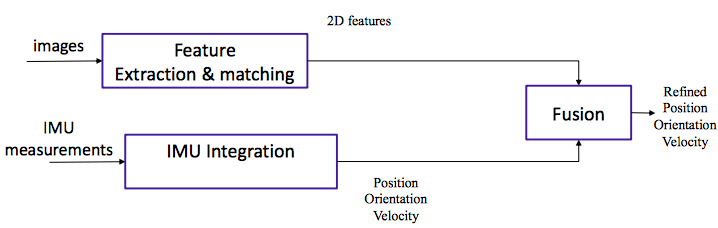
\includegraphics[scale=0.6]{pics/tight}
\caption{Tightly Coupled Approach.}
\end{center}
\end{figure}
System states are:
\begin{itemize}
\item \textbf{Tightly Coupled:} $X=\begin{pmatrix}
p_W(t);q_{WB}(t);v_W(t);b^a(t);b^g(t);L_{w,1};\hdots;L_{w,K}\end{pmatrix}$, with $L$ Landmarks.
\item \textbf{Loosely Coupled} $X=\begin{pmatrix}
p_W(t);q_{WB}(t);v_W(t);b^a(t);b^g(t)\end{pmatrix}$
\end{itemize}
\end{answer}
\item \textit{How can we use non-linear optimization-based approaches to solve for visual inertial fusion (mathematical expression and graphical illustration of the pose graph)?}
\begin{answer}
\textbf{Maximum a Posterior Estimation (MAP)}: Fusion solved as a non-linear optimization problem. Increased accuracy over filtering methods. We have
\begin{equation}
x_k=f(x_{k-1}), \quad z_k=h(x_{i_k},l_{i_j}),
\end{equation}
where $X$ are the robot states, $L$ the 3D points and $Z$ the features and IMU measurements. It holds
\begin{equation}
\begin{split}
\{X^*,L^*\}&=\text{argmax}_{X,L}P(X,L|Z)\\
&=\text{argmin}_{X,L}\{ \underbrace{\sum_{k=1}^N ||f(x_{k-1})-x_k||_{\Lambda_k}^2}_{\text{IMU residuals}}+\underbrace{\sum_{i=1}^M ||h(x_{i_k})-z_i||_{\Sigma_i}^2}_{\text{Reprojection residuals}}\}
\end{split}
\end{equation}
An open problem is consistency: 
\begin{itemize}
\item Filters: Linearization around different values of the same variable may lead to error.
\item Smoothing methods: may get stuck in local minima.
\end{itemize}
\begin{figure}[h]
\begin{center}
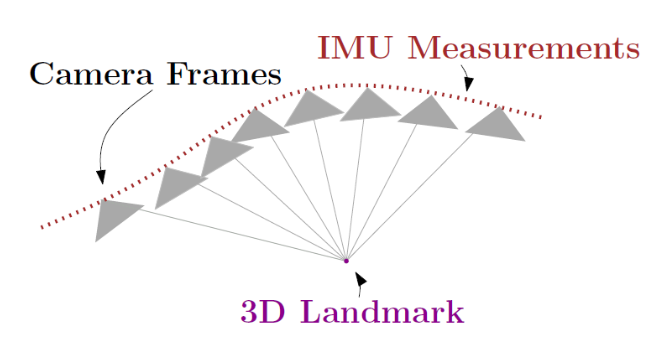
\includegraphics[scale=0.4]{pics/map}
\caption{Max a Posterior Estimation (MAP).}
\end{center}
\end{figure}
\end{answer}
\end{enumerate}
\newpage
\section*{Lecture 14 Event-based Vision}
\begin{enumerate}
\item \textit{What’s a DVS and how does it work? }
\begin{answer}
Event cameras enable \textbf{low-latency sensory motor control $<1ms$}.  A DVS outputs \textbf{asynchronous} events at microsecond resolution. An event is generated each time a single pixel detects an \textbf{intensity changes}:
\begin{equation}
\text{event:} \langle t,<x,y>,\text{sign}\left(\frac{\text{d}I(x,y)}{\text{d}t} \right)\rangle
\end{equation}
All pixels are independent from another. Implements \textbf{level-crossing} sampling. Reacts to \textbf{logarithmic} brightness changes. Each pixel is independent of all the other pixels. Events are generated everytime a single pixel sees a change of the logarithm of the brightness that is equal to $C$, i.e.
\begin{equation}
|\log(I)|=|\log(I(t+\Delta t)-\log(I(t))|=C,
\end{equation}
where $C \in [0.15,0.20]$ is called \textbf{contrast sensitivity} and can be tuned by the user. Since brightness can be either positive or negative, we have ON event if $=C$ and OFF event if $=-C$.
\begin{figure}[tbh]
\begin{center}
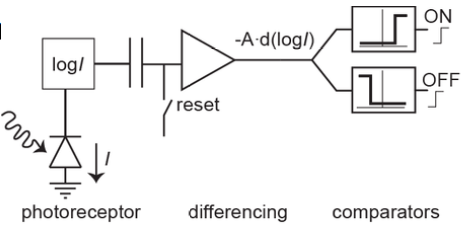
\includegraphics[scale=0.6]{pics/dvsel}
\caption{DVS circuit}
\end{center}
\end{figure}
\begin{figure}[tbh]
\begin{center}
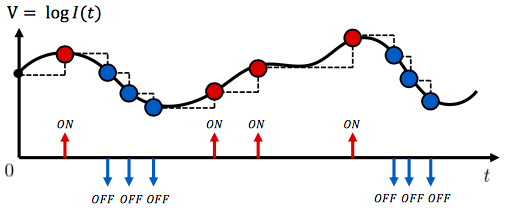
\includegraphics[scale=0.6]{pics/dvs}
\caption{DVS.}
\end{center}
\end{figure}
Traditional sampling is performed with the discriminant (time) on $x-$axis. Level-crossing sampling works with the change in intensity, in the $y-$axis.
\end{answer}

\item \textit{What are its pros and cons vs standard cameras and vs high speed cameras? }
\begin{answer}
\
\textbf{Advantages:}
\begin{itemize}
\item Low latency (1 micro second)
\item High dynamic range (140 dB instead of 60 dB)
\item Low power: 10mW instead of 1W
\end{itemize}
\textbf{Disadvantages:}
\begin{itemize}
\item Paradigm shift: requires totally new vision algorithms
\begin{itemize}
\item Asynchronus pixels,
\item No intensity information (only binary intensity changes).
\end{itemize}
\end{itemize}

\end{answer}
\item \textit{ Can we apply standard camera calibration techniques? }
\begin{answer}
The standard pinhole camera model is still valid (same optics). Standard passive calibration cannot be used: we would need to move the camera. \textbf{Blinking patterns} (computer screen, LEDs).
\end{answer}
\item \textit{How can we compute optical flow with a DVS?}
\begin{answer}
White pixels become black, i.e. the brightness decrease, i.e. negative events (black color). Events are represented by dots. At what speed is the edge moving? $v=\frac{\Delta x}{\Delta t}$. 
Two different approaches
\begin{itemize}
\item \textbf{Event-by-event processing} (i.e. estimate the state event by event): Pros: low latency, Cons: with high speed motion, there are dozens of millions of events per seconds (GPU)\\
Let's start with an approximation:
\begin{equation}
\begin{split}
\Delta \log(I)&=\frac{\partial \log(I)}{\delta t}\Delta t\\
&=\frac{1}{I}\frac{\delta I}{\delta t}\Delta t\\
&=\frac{\partial I}{I}.
\end{split}
\end{equation}


\item \textbf{Event-packet processing} (i.e. process the last $N$ events): Pros: $N$ can be tuned to allow real-time performance on a CPU. Cons: no longer microsecond resolution (when is this really necessary=)
\end{itemize}


\end{answer}
\item \textit{Intuitive explanation of why we can reconstruct the intensity. }
\begin{answer}
The intensity signal at the event time can be reconstructed by integration of $\pm C$. Given the events and the camera motion (rotation), recover the absolute brightness. \textbf{Explanation:} An event camera naturally responds to edges, hence, if we know the motion, we can relate the events to world coordinates to get an edge/gradient map. Then, just integrate the gradient map to get absolute intensity.
\begin{enumerate}
\item Recover the gradient map of the scene. Let $L=\log(I)$. Then
\begin{equation}
\Delta L(t)=L(t)-L(t-\Delta t)=C.
\end{equation}
In terms of the brightness map $M(x,y)$:
\begin{equation}
M(p_m(t))-M(p_m(t-\Delta t))\approx g\cdot v\cdot \Delta t,
\end{equation}
with $g=\nabla M(p_m(t))$.
\item Integrate the gradient to obtain brightness. Poisson reconstruction: integrate the gradient map $g$ to get absolute brightness $M$.
\begin{figure}[tbh]
\begin{center}
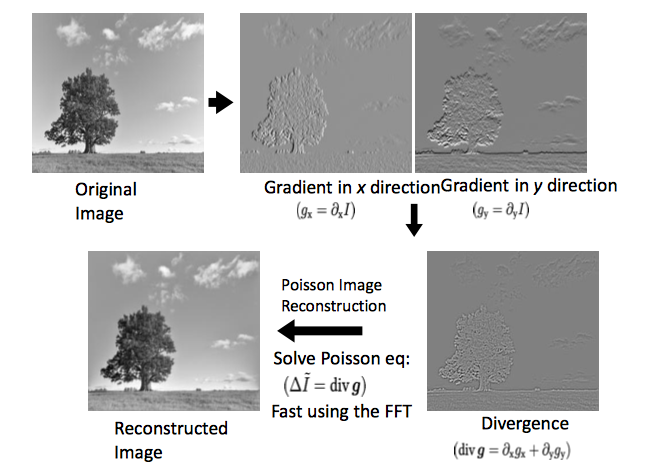
\includegraphics[scale=0.6]{pics/poisson}
\caption{DVS vs High Speed Cameras.}
\end{center}
\end{figure}
\end{enumerate}
\end{answer}
\item \textit{What is the generative model of a DVS? }
\begin{answer}
???
\end{answer}
\item \textit{What is a DAVIS sensor?}
\begin{answer}
Combines an event sensor (DVS) with a standard camera in the same pixel array. Output are frames (at 30 Hz) and events (asynchronous). One can them perform SLAM with an IMU, which increases robustness and accuracy. \\
Open problems for DVS are: noise modeling, asynchronous feature and object detection and tracking, sensor fusion, asynchronous learning and recognition, estimation and control, low power computation.

\end{answer}
\item \textit{ Can you write the equation of the event generation model and its proof?}
\begin{answer}
To simplify the notation, let's assume that $I(x,y,t)=\log(I(x,y,t))$. Consider a given pixel $p(x,y)$ moving with apparent motion $\vec{u}=(u,v)$ (i.e. induced by a moving 3D patch). It can be shown, that an event is generated if the scalar product between the gradient and the appearent motion vector $u$ is equal to $C$.
\begin{equation}
-\nabla I \cdot u=C
\end{equation}
\begin{proof}
The proof comes from the brightness constancy assumption, which says that the intensity value of $p$, before and after the motion, must remained unchanged
\begin{equation}
I(x,y,t)=I(x+u,y+v,t+\Delta t)
\end{equation}
By replacing the right-hand term by its first order approximation at $t+\Delta t$, we get
\begin{equation}
\begin{split}
I(x,y,t)&=I(x,y,t+\Delta t)+ \frac{\partial I}{\partial x}u+\frac{\partial I}{\partial y}v\\
I(x,y,t+\Delta t)-I(x,y,t)&=-\frac{\partial I}{\partial x}u-\frac{\partial I}{\partial y}v\\
\Rightarrow \Delta I &= C= -\nabla \cdot u.
\end{split}
\end{equation}
This equation described the linearized event generation equation for an event generated by a gradient $\nabla I$ that moved by a motion vector $u$ (optical flow) during a time interval $\Delta t$. 1 Equation, 2 Unknowns, solution is to add events.
\end{proof}
\end{answer}
\end{enumerate}
\newpage
\newpage
\section*{Lecture 15 Visual (inertial) Odometry}
\begin{enumerate}
\item \textit{List one or more possible ways to decide when to triangulate new landmarks based on feature tracks.}
\begin{answer}
Triangulate new landmarks when
\begin{itemize}
\item Angle between landmark and camera is sufficient.
\item Keypoints were tracked over certain number of frames.
\end{itemize}
\end{answer}
\item \textit{What are keyframes in Visual Odometry? }
\begin{answer}
\
\begin{itemize}
\item Frames, where new landmarks are triangulated.
\end{itemize}
\end{answer}
\item \textit{Why are they needed? Are they strictly necessary?}
\begin{answer}
\
\begin{itemize}

\item For BA, you can optimize only on desired frames.
\item Reduces computational complexity without reducing accuracy.
\end{itemize}
\end{answer}
\item \textit{How to decide whether a given frame should be a keyframe?}
\begin{answer}
\begin{itemize}
\item Possible to use every frame as keyframe in a continuous manner rather than discrete, by keeping track of first observation of landmarks (and pose) and triangulate, if angle large enough.
\end{itemize}
\end{answer}
\item \textit{Do you know any popular Visual (Inertial) Odometry algorithm? (one or more). Can you explain briefly how they work?}
\begin{answer}
Kalman filtering Visual odometry (see MSCKF for planetary landing I quoted in the final report). It fuses in a probabilitistc framework both observations from the camera with predictions from an IMU. It can be coupled with GPS (for UAVs for example).\\
About MSCKF (Multi-state constraint kalman filter): its particularity is that observations from the camera do not need to triangulate keypoints, so they don't need to be added to the state, reducing the memory/computation requirements. Also, only a sliding window of observations (2D pts) is kept for each keypoint, reducing the  complexity.
\end{answer}
\item \textit{Suppose you have implemented a monocular Visual Odometry pipeline. How would change it to work as well with a stereo camera?}
\begin{answer}
\
\begin{enumerate}
\item You fuse it in a Kalman filter and don't change much, by taking observations of both cameras as observations with same processing and weights (only take care of offset).
\item Remove triangulation from normal pipeline and triangulate new keypoints each time using the 2 cameras, but would be pretty bad with its accuracy.
\item Triangulate each time and refine the poses of the 3d pts until the interrsection of bundles (such as inSVO I think, and for event cameras algorithms) is precise enough (by computing/refining the uncertainty each time) until the 3d pts positions are very precise, in which case they're added to sparse map and used in odometry (P3P).
\end{enumerate}
\end{answer}
\end{enumerate}
\newpage
\section*{Application Questions}
\begin{enumerate}
\item \textit{Summarize the building blocks of a visual odometry (VO) or visual SLAM (VSLAM) algorithm}.
\begin{answer}
In general the are three different VO algorithms:
\begin{itemize}
\item 2D-2D: Compute Essential/Fundamental matrix between images and extract extrinsics, then concatenate relative movements.
\item 3D-3D: Determine the aligning transform of two 3D landmark sets, then concatenate.
\item 3D-2D: Use PnP to estimate absolute pose from known 3D landmarks and their most recent observation. No concatenation necessary!
\end{itemize}
The detailed architecture of a 3D-2D VO is the following:
\begin{enumerate}
\item \textbf{Bootstrapping:}
\begin{enumerate}
\item Initialize the algorithm by detecting and matching features in two frames. Use correspondences to triangulate a first set of landmarks.
\end{enumerate}
\item \textbf{Continuous Operation} (Feature-based):
\begin{enumerate}
\item Track or match features from previous image to get the correspondence of current 2D features to 3D landmarks.
\item Motion estimation by using RANSAC and Perspective from 3 Points (P3P). Use the 2D-3D correspondances.
\item Add additional candidate keypoints and landmarks over the next images. Triangulate new candidate landmarks from original observation and keyframe observation. To derermine if a landmark can be triangulated with sufficient accuracy, determine base line/bearing angle between the two observations. If this measure reaches some threshold, add candidate landmark to the landmarks used for motion estimation (PnP). Detect new features to track over the next images.
\end{enumerate}
\item \textbf{(VSLAM) only}:
\begin{enumerate}
\item Loop detection: use place recognition by BoW or other algorithms to update landmarks and transformations to align with loop closure.
\item Local Graph optimization: Refine graph by minimizing the reprojection error of landmarks over all frames in which they were observed. The argument over which is minimized are the camera poses.
\end{enumerate}
\end{enumerate}
\end{answer}
\item \textit{Augmented reality (AR) is a view of a physical scene augmented by computer-generated sensory inputs, such as data or graphics. Suppose you want to design an augmented reality system that super-imposes text labels to the image of real physical objects. Summarize the building blocks of an AR algorithm.}
\begin{answer}
\
\begin{enumerate}
\item Use SfM (Multiple View Geometry) to create 3D scene reconstruction.
\begin{enumerate}
\item Option 1: Use features such as Harris, FAST or others and match them over subsequent frames. Use correspondences to extract extrinsics by PnP.
\item Option 2: Use checkerboard and extract homographies. Use homographies to compute extrinsics (position). This is essentially Zhang's camera calibration approach.
\end{enumerate}
\item Assign some set of landmarks to an object. which should be labelled. Possibly use markers (e.g. April Tags) to identify objects that should be augmented.
\item For subsequent images: track keypoints that correspond to scene landmarks.
\item Add text label output image and position every label to the centroids of all keypoints that belong to (some set of landmarks / some distinct object).
\end{enumerate}
\end{answer}
\item \textit{Suppose that your task is to reconstruct an object from different views. How do you proceed?}
\begin{answer}
\
\begin{enumerate}
\item \textbf{Sparse reconstruction} (only features, no smooth surface):\\
Do we know the relative position of the viewpoints?
\begin{enumerate}
\item \textbf{YES} (stereo vision, sequential SfM): Get the 2D-2D correspondences by extracting and matching features. Use correspondences to determine relative camera poses and triangulate landmarks. Track keypoints over subsequent frames and use landmark-keypoint correspondences to determine the camera poses. Extract and triangulate additional landmarks if their base line / bearing angle allows sufficient accuracy.
\item \textbf{NO} (structure from motion, hierarchical SfM): Get 2D-2D correspondences by extracting and matching features. Estimate fundamental/essential matrix (8 point algorithm) and decompose $E$ into $R$ and $t$. Use correspondences and relative camera poses to triangulate landmarks. 
\end{enumerate}
\item \textbf{Dense reconstruction} (dense region of pixels, smooth surface, preferred)
\begin{enumerate}
\item Choose reference image.
\item For every pixel in the reference image, calculate aggregated photometric error as a function of depth.
\item The photometric error of a pixel is the reprojection error that results if we reporoject the point to some other image (depending at what depth we set the point). We get it evaluating the (SSD,SAD,NCC) difference of a patch from all patches on the same epipole from another point of view.
\item Aggregated photometric error is the sum of error functions from all further images. The best depth estimate for a pixel in the reference image will minimize the aggregated photometric error function.
\item Evaluate Disparity Space Image (DSI) by combining all error functions of all pixels in a 3D error funcion depending on ($u$,$v$ and depth).
\item Global Regularization: Ensure smoothness by penalizing non-smooth areas and minimizing global energy.
\end{enumerate}
\end{enumerate}
\end{answer}
\item \textit{Building a panorama stitching application. Summarize the building blocks}.
\begin{enumerate}
\item \textbf{Feature Extraction:} find distinct features that are independent of changes in scale, rotation, illumination or viewpoint angle (e.g. corner or blobs).
\item \textbf{Feature Description}: Establish descriptors for all features. (binar descriptors, census transform, intensity patches,...).
\item \textbf{Feature Matching}: Use difference measure (SSD,SAD,NCC) to find close features.
\item \textbf{Optional RANSAC:} Use RANSAC to filter outlier matches.
\item \textbf{Feature Alignment}: Scale, rotate and warp images to align as many feature matches as possible.  
\end{enumerate}
\item \textit{How would you design a mobile tourist app? The user points the phone in the direction of a landmark and the app displays tag with the name of it. How would you implement it?}
\begin{enumerate}
\item Indexing: use of landmarks to create image Bag Of Words index for each landmark.
\item Place recognition: compare camera image to image index and identify if any of the landmarks is present.
\item AR: If some landmarks is present, use the BoW inde to identify keypoints in the camera image that correspond to the landmark. Display tag with the name of the landmark located in the centroid of all keypoints identified to belong to some landmark.
\end{enumerate}
\item \textit{Assume that we have several images downloaded from flicker showing the two towers of Grossmünster. Since such images were uploaded by different persons they will have different camera parameters (intrinsic and extrinsic), different lighting, different resolutions and so on. If you were supposed to create a 3D model of Grossmünster, what kind of approach would you use? Can you get a dense 3D model or it will be a sparse one? Please explain the pipeline that you propose for this scenario.}
\begin{enumerate}
\item Hierarchical SfM:
\begin{enumerate}
\item Identify clusters of nearby images by extracting and matching features.
\item Perform SfM for every cluster and build point cloud.
\item Merge clusters pairwise and refine poses and structure by minimiting the reprojection errors of landmarks across different viewpoints.
\end{enumerate}
\end{enumerate}
\item \textit{Assume that you move around a statue with a camera and take pictures in a way that the statue is not far from the camera and always completely visible in the image. If you were supposed to find out where the pictures were taken, what would you do with the images? What kind of approach would you use? Since the camera motion is around the statue, the images contain different parts of the statue. How do you deal with this problem?}
\begin{enumerate}
\item Feature matching across sequential frames.
\item Estimate relative motion between frames using 2D-2D correspondences (8 point, 5 point algorithms) and extracting $R$ and $t$ from the Fundamental matrix (uncalibrated!) or the Essential matrix (calibrated!).
\item Optional: refine poses when a loop is detected and features from the first image are detected.
\end{enumerate}
\item \textit{Suppose that you have two robots exploring an environment, explain how the robots should localize themselves and each other with respect to the environment? What are the alternative solutions?}
\begin{enumerate}
\item \textbf{Localization:}
\begin{enumerate}
\item Monocular Visual SLAM or Stereo Camera Visual SLAM for drift resistant odometry and map building (to prevent drift).
\item IMU for accurate localization and to add absolute scale to the localization.
\item GPS to improve global accuracy.
\item Laser triangulation sensor for map building (LIDAR)
\item Combine multiple of these options and use a filter to get the final localization (e.g. Kalman Filter).
\end{enumerate}
\item \textbf{Communication}
\begin{enumerate}
\item Wirelessly share built maps and current position.
\item Possibly visual tracking and recognition of close robots using markers or other templates.
\item Possibly measurement of distance and heading of close robots by radio transmission (measure time and signal direction).
\end{enumerate}
\end{enumerate}
\end{enumerate}
\newpage
\section{Mini Project Exam Preparation}
\end{document}
